\documentclass[a4paper,12pt]{report}

\usepackage[utf8]{inputenc}
\usepackage{fontenc}
% \usepackage[french, arabic]{babel} % If you write in French

\usepackage{a4wide}
\usepackage{graphicx}
\usepackage{placeins}
%pour la mise en page des tableaux
\usepackage{graphicx}
\usepackage{placeins}
\usepackage{rotating}
\usepackage{array}
\usepackage{lipsum}
\usepackage{algorithmic}

\usepackage{tabularx}
\usepackage[table,xcdraw]{xcolor}
\usepackage{wrapfig}
\usepackage{subcaption}
\usepackage{color, colortbl}
\definecolor{Gray}{gray}{0.9}
\definecolor{LightCyan}{rgb}{0.88,1,1}
\usepackage{longtable}
\usepackage{float}
\usepackage{array} % for 

\usepackage{amsthm}
\usepackage{amssymb,amsmath,bbm}
\usepackage{fontspec}          % For font management in XeLaTeX
\usepackage{unicode-math}      % Allows math font selection
\usepackage[footnote]{acronym}

% Set a math font that supports all symbols
\setmathfont{Latin Modern Math}
\usepackage{xcolor}
\usepackage{tcolorbox}
\usepackage{lscape}
\usepackage{afterpage}
\usepackage{rotating}
\usepackage[nottoc,notlof,notlot]{tocbibind}
\usepackage{tocloft}
\usepackage{pdfpages}
\graphicspath{{images/}{images_pfe/}{img_pfe/}}
\newlength\figureheight
\newlength\figurewidth
\usepackage{ifthen}
\usepackage{ifpdf}
\ifpdf
\usepackage[pdftex]{hyperref}
\else
\usepackage{hyperref}
\fi
\usepackage{color}
\hypersetup{%
colorlinks=true,
linkcolor=black,
citecolor=black,
urlcolor=blue}
% \urlstyle{same}
\usepackage[top=2.5cm,bottom=2.5cm,right=2.5cm,left=2.5cm]{geometry}
\usepackage{changepage}

\usepackage{tabularx}
    \newcolumntype{L}{>{\raggedright\arraybackslash}X}
\usepackage{longtable}
% \usepackage{tabularx}
%     \newcolumntype{L}{>{\raggedright\arraybackslash}X}
% \usepackage{longtable}

\usepackage{xltabular}
\renewcommand{\tablename}{Table}
\renewcommand{\figurename}{Figure}

% Colors package
\usepackage[table]{xcolor}
\usepackage{xcolor}

\definecolor{lightblue}{rgb}{0.74, 0.83, 0.9}

% Colors for tables package
\usepackage{colortbl}



\usepackage{tikz}
\usetikzlibrary{arrows,shapes,positioning,shadows,trees}
\usetikzlibrary{shapes.geometric, arrows.meta, positioning}

\tikzset{
  basic/.style  = {draw, text width=2cm, drop shadow, font=\sffamily, rectangle},
  root/.style   = {basic, rounded corners=2pt, thin, align=center,
                   fill=blue!30},
  level 2/.style = {basic, rounded corners=6pt, thin,align=center, fill=blue!60,
                   text width=8em},
  level 3/.style = {basic, thin, align=left, fill=blue!10, text width=6.5em}
}



% For the dark red color used for the points
\usepackage{xcolor} 
\definecolor{darkred}{rgb}{0.6,0,0}


% --- End of Bibliography Setup ---
%% pour la numération des sous sou sections
\setcounter{tocdepth}{2}
\setcounter{secnumdepth}{2}



% pour les algorithmes
\usepackage[ruled,vlined,linesnumbered]{algorithm2e}
\DontPrintSemicolon

\setlength\arrayrulewidth{1pt}
\renewcommand{\baselinestretch}{1.05}
\usepackage{fancyhdr}
\pagestyle{fancy}
\fancyhf{}
\lhead{\bfseries\nouppercase{\leftmark}}
\rfoot{\bfseries\thepage}
\setlength{\headheight}{14.5pt}

\let\headruleORIG\headrule

\renewcommand{\headrule}{\color{black} \headruleORIG}
\renewcommand{\headrulewidth}{1.0pt}
\usepackage{colortbl}
\arrayrulecolor{black}

\fancypagestyle{plain}{
  \fancyhead{}
  \fancyfoot[R]{\bfseries\thepage}
  \renewcommand{\headrulewidth}{0pt}
}


\makeatletter
\def\@textbottom{\vskip \z@ \@plus 1pt}
\let\@texttop\relax
\makeatother

\makeatletter
\def\cleardoublepage{\clearpage\if@twoside \ifodd\c@page\else%
  \hbox{}%
  \thispagestyle{empty}%
  \newpage%
  \if@twocolumn\hbox{}\newpage\fi\fi\fi}
\makeatother


\usepackage{array}
\usepackage{bm}
\usepackage{multirow}
% \usepackage[footnote]{acronym}

\usepackage[bottom]{footmisc}

% Use polyglossia for languages with XeLaTeX/LuaLaTeX
\usepackage{polyglossia}
\setmainlanguage{english}
\setotherlanguage{french}
\setotherlanguage{arabic}
\usepackage{lipsum}
% --- Complete Bibliography Setup ---

% 1. Load biblatex with the core style options
\usepackage[
    backend=biber,
    style=authoryear,       % Use author-year style
    maxcitenames=1,         % Use "et al." if more than 1 author
    doi=false,              % Your custom settings from before
    isbn=false,
    eprint=false,
    uniquelist=false
]{biblatex}

% 2. Link your .bib file
\addbibresource{references.bib}


% 3. This block changes citation parentheses to square brackets (works on older systems)
\usepackage{xpatch} % Make sure this package is loaded

% 4. Your other commands (non-italic "et al.", remove URLs, etc.)
\DefineBibliographyStrings{english}{%
  andothers = {et\addabbrvspace al\adddot},
}


% 5. Your command to remove URLs from the final reference list
\AtEveryBibitem{
  \ifentrytype{misc}{
  }{
    \clearfield{url}
    \clearfield{urlyear}
  }
}

\newtheoremstyle{break}
  {11pt}{11pt}%
  {\itshape}{}%
  {\bfseries}{}%
  {\newline}{}%
\theoremstyle{break}

%\theoremstyle{definition}
\newtheorem{definition}{Définition}[chapter]

%\theoremstyle{definition}
\newtheorem{theoreme}{Théorème}[chapter]

%\theoremstyle{remark}
\newtheorem{remarque}{Remarque}[chapter]

%\theoremstyle{plain}
\newtheorem{propriete}{Propriété}[chapter]
\newtheorem{exemple}{Exemple}[chapter]

%table break line

\usepackage{makecell}

\renewcommand\theadalign{bl}
\renewcommand\theadfont{\bfseries}
\renewcommand\cellalign{bl}
\renewcommand\cellgape{\Gape[2pt]}

\parskip=5pt
%\sloppy
 %%%%********************************************************************
\usepackage{xcolor}
\definecolor{quotemark}{gray}{0.7}
\makeatletter
\def\fquote{%
    \@ifnextchar[{\fquote@i}{\fquote@i[]}%]
           }%
\def\fquote@i[#1]{%
    \def\tempa{#1}%
    \@ifnextchar[{\fquote@ii}{\fquote@ii[]}%]
                 }%
\def\fquote@ii[#1]{%
    \def\tempb{#1}%
    \@ifnextchar[{\fquote@iii}{\fquote@iii[]}%]
                      }%
\def\fquote@iii[#1]{%
    \def\tempc{#1}%
    \vspace{1em}%
    \noindent%
    \begin{list}{}{%
         \setlength{\leftmargin}{0.1\textwidth}%
         \setlength{\rightmargin}{0.1\textwidth}%
                  }%
         \item[]%
         \begin{picture}(0,0)%
         \put(-15,-5){\makebox(0,0){\scalebox{3}{\textcolor{quotemark}{``}}}}%
         \end{picture}%
         \begingroup\itshape}%
 %%%%********************************************************************
 \def\endfquote{%
 \endgroup\par%
 \makebox[0pt][l]{%
 \hspace{0.8\textwidth}%
 \begin{picture}(0,0)(0,0)%
 \put(15,15){\makebox(0,0){%
 \scalebox{3}{\color{quotemark}''}}}%
 \end{picture}}%
 \ifx\tempa\empty%
 \else%
    \ifx\tempc\empty%
       \hfill\rule{100pt}{0.5pt}\\\mbox{}\hfill\tempa,\ \emph{\tempb}%
   \else%
       \hfill\rule{100pt}{0.5pt}\\\mbox{}\hfill\tempa,\ \emph{\tempb},\ \tempc%
   \fi\fi\par%
   \vspace{0.5em}%
 \end{list}%
 }%
 \makeatother
 %%%%********************************************************************
 \usepackage{background}
% \backgroundsetup{scale = 0.5,angle = 0, opacity = 1, contents = {
\includegraphics[scale = 0.65 ]{bg.jpg}}}
\backgroundsetup{
  angle=0,        % Rotate image to make it vertical
  opacity = 0.9,
  position=current page.south west, 
  vshift=10cm,      % Move it up from the bottom
  hshift=14.2cm,      % Move it right from the left margin
  contents={
\includegraphics[scale = 0.65]{images_pfe/bg_uh2c.jpg}}
}
 \usepackage{afterpage}

\newcommand\blankpage{%
    \null
    \thispagestyle{empty}%
    \addtocounter{page}{-1}%
    \newpage}
    
\renewcommand{\listalgorithmcfname}{Liste des algorithmes}
\setmainlanguage{english}
\setotherlanguage{arabic}
\newfontfamily\arabicfont[Script=Arabic,Scale=1.3]{Scheherazade}

\newcommand{\mychapter}[2]{
    
    \chapter*{#2}
    \addcontentsline{toc}{chapter}{#2}
}


\usepackage[page,toc,titletoc,title]{appendix}

\addto\captionsfrench{%
  \renewcommand\appendixname{Annexe}
  \renewcommand\appendixpagename{Annexes}
  \renewcommand{\appendixtocname}{Annexes}
}
\usepackage{etoolbox}
\appto\appendix{\addtocontents{toc}{\protect\setcounter{tocdepth}{0}}}

% reinstate the correct level for list of tables and figures and algorithms
\appto\listoffigures{\addtocontents{lof}{\protect\setcounter{tocdepth}{1}}}
\appto\listoftables{\addtocontents{lot}{\protect\setcounter{tocdepth}{1}}}
\appto\listofalgorithms{\addtocontents{loa}{\protect\setcounter{tocdepth}{1}}}

\usepackage{xpatch} 
\usepackage{textcomp}
\AtBeginDocument{%
 
  \xpatchbibmacro{parencite}
    {\bibopenparen}
    {\bibopenbracket}
    {}{}
  \xpatchbibmacro{parencite}
    {\bibcloseparen}
    {\bibclosebracket}
    {}{}
}

\begin{document}

\begin{titlepage}
    \centering

    
\begin{minipage}{0.4\textwidth}
    \begin{flushleft}
        
\includegraphics[width=3cm]{fsbm-removebg.png}
        \hspace*{-0.2cm} % Adjust negative space to bring logos closer
        
\includegraphics[width=3cm]{images_pfe/dsbd.png}
    \end{flushleft}
\end{minipage}\hfill
\begin{minipage}{0.5\textwidth}
    \begin{flushright}
        
\includegraphics{images_pfe/AIM-UNESCO_EN.png}
    \end{flushright}
\end{minipage}

    \vspace{1cm} % Reduced vertical space

    % --- DEGREE INFORMATION ---
   {\large \bfseries PFE: End-of-Studies Project }\\[5mm]
    {\large Submitted for the attainment of the degree:}\\[5mm]
    {\large \bfseries MASTER Data Science \& BIG Data}\\[5mm]
    \textbf{Option:} {\large Data Science}

    \vspace{0.5cm} % Reduced vertical space

    % --- TITLE ---
    \rule{\linewidth}{0.3mm} \\[0.4cm]
    { \huge \bfseries Enhancing Multi-Agent Reinforcement Learning under
    Partial Observability via Learning-Informed Masking\\[0.2cm] }
    \rule{\linewidth}{0.3mm}

    \vspace{1cm} % Reduced vertical space

    % --- AUTHOR AND SUPERVISORS ---
    \begin{minipage}{0.48\textwidth}
        \begin{flushleft} \large
            \emph{Realized by:}\\
            Mrs. \textsc{Amghar} Hind
        \end{flushleft}
    \end{minipage}\hfill
    \begin{minipage}{0.48\textwidth}
        \begin{flushleft} \large % Using flushleft for better alignment
            \emph{Supervised by:} \\
            Pr. \textsc{Sael} Nawal  \\
            \textit{- Academic Supervisor}\\[3mm]
            Mme. \textsc{El Khamlichi} Btissam \\
            \textit{- Industrial Supervisor}
           
           


        \end{flushleft}
    

    \end{minipage}

    \vfill % Pushes content to the bottom, ensuring it all fits

    % --- JURY INFORMATION ---
    {\large \textit{Presented on July 21st, 2025, before the jury composed of:}}\\[5mm]

%  \begin{tabular}{ll}
%     \large Pr. Nawal \textsc{Sael} & \large - Academic Supervisor \\
%     % \large Pr. Nabil \textsc{Aharrane} & \large - Co-supervisor \\
%     \large Pr. Nouh \textsc{Said} & \large - Membre de jury \\
%     \large Pr. Sadiq \textsc{Mounir} & \large - Membre de jury \\
%     \large Pr. Sekhara \textsc{Youssef} & \large - Membre de jury \\
%     \large Pr. Kendali \textsc{Khalid} & \large - Membre de jury \\
%     \large Dr. Taoufik \textsc{Amzil} & \large - Membre de jury \\
% \end{tabular}
\begin{tabular}{ll}
   
    \large Pr. \textsc{Kendali} Khalid & \large - President \\
    \large Pr. \textsc{Nouh} Said & \large - Examiner \\
    \large Pr. \textsc{Sadiq}  Mounir & \large - Examiner \\
    \large Pr. \textsc{Sekhara} Youssef & \large - Examiner \\
   
 
    \large Pr. \textsc{Sael} Nawal  & \large - Academic Supervisor \\
\end{tabular}

    \vspace{1cm} % Reduced vertical space

    % --- FOOTER ---
    {\large Academic Year: 2024/2025}

\end{titlepage}
% \mychapter{0}{Acknowledgements}

% I would like to express my sincere gratitude to those who have supported and guided me throughout this project.
% \medskip

% First, I would like to thank my academic supervisor, \textbf{Pr. Nawal SAEL}, for her invaluable guidance, insightful feedback, and constant encouragement. Your expertise played a crucial role in shaping the direction and enhancing the quality of this research.
% \medskip

% % I am also deeply grateful to the members of my jury for taking the time to review this work. My thanks go to my co-supervisor, \textbf{Pr. Nabil AHARRANE}, and to the examiners, \textbf{Pr. Nouh SAID} and \textbf{Pr. Sadiq MOUNIR}, for their willingness to share their expertise on this project.
% % \medskip
% I am also deeply grateful to the members of my jury for taking the time to review this work. My thanks go to  the examiners \textbf{Pr. Nouh SAID} and \textbf{Pr. Sadiq MOUNIR}, for their willingness to share their expertise on this project.
% \medskip

% Special thanks to \textbf{Professor El Khamlichi Btissam} for her support and mentorship. Your enthusiasm and constructive advice have been a source of motivation and have helped me to overcome various challenges during this project.


% \medskip
% Additionally, I would like to express my deep gratitude to \textbf{Reda El Marhouch, and Fadoua Ait Ayane}, Their guidance and support have laid a strong foundation for my research. Their contributions have not only enriched my academic development but have also inspired and encouraged me throughout this project. I am truly thankful for their kindness and dedication.

% \medskip
% Special thanks to all my teachers at the Faculty of Sciences Ben M'Sick (FSBM) for providing the foundational knowledge that made this work possible.
% \medskip

% Finally, I extend my deepest thanks to my family and friends for their immense support and encouragement throughout this journey. I am eternally grateful to my wonderful mother and father, for their unconditional love and belief in me. Your support has been a constant source of inspiration.

% \medskip
% This project would not have been possible without the collective efforts and support of these remarkable individuals. Thank you all for your contributions and dedication.



% \clearpage

% \mychapter{0}{Acknowledgements}

% I would like to express my sincere gratitude to those who have supported and guided me throughout this project.
% \medskip

% First, I would like to thank my academic supervisor, \textbf{Pr. Nawal SAEL}, for her invaluable guidance, insightful feedback, and constant encouragement. Your expertise played a crucial role in shaping the direction and enhancing the quality of this research.
% \medskip

% I am also deeply grateful to the members of my jury for taking the time to review this work. My thanks go to the examiners \textbf{Pr. Nouh SAID}, \textbf{Pr. Sadiq MOUNIR}, and \textbf{Dr. Taoufik AMZIL}, as well as the jury members \textbf{Pr. Sekhara YOUSSEF} and \textbf{Pr. Kendali KHALID}, for their willingness to share their expertise on this project.
% \medskip

% Special thanks to \textbf{Professor El Khamlichi Btissam} for her support and mentorship. Your enthusiasm and constructive advice have been a source of motivation and have helped me to overcome various challenges during this project.
% \medskip

% Additionally, I would like to express my deep gratitude to \textbf{Reda El Marhouch} and \textbf{Fadoua Ait Ayane}. Their guidance and support have laid a strong foundation for my research. Their contributions have not only enriched my academic development but have also inspired and encouraged me throughout this project. I am truly thankful for their kindness and dedication.
% \medskip

% Special thanks to all my teachers at the Faculty of Sciences Ben M'Sick (FSBM) for providing the foundational knowledge that made this work possible.
% \medskip

% Finally, I extend my deepest thanks to my family and friends for their immense support and encouragement throughout this journey. I am eternally grateful to my wonderful mother and father for their unconditional love and belief in me. Your support has been a constant source of inspiration.
% \medskip

% This project would not have been possible without the collective efforts and support of these remarkable individuals. Thank you all for your contributions and dedication.

% \clearpage

% \mychapter{0}{Acknowledgements}

% I would like to express my sincere gratitude to those who have supported and guided me throughout this project.
% \medskip

% First, I would like to thank my academic supervisor, \textbf{Pr. \textsc{Sael} Nawal}, for her invaluable guidance, insightful feedback, and constant encouragement. Your expertise played a crucial role in shaping the direction and enhancing the quality of this research.
% \medskip

% I am also deeply grateful to the members of my jury for taking the time to review this work. My sincere thanks go to the President of the jury, Pr. \textbf{\textsc{Kendali} Khalid}, and to the examiners: \textbf{Pr. \textsc{Nouh} Said}, \textbf{Pr. \textsc{Sadiq} Mounir}, \textbf{Pr. \textsc{Sekhara} Youssef}, and \textbf{Dr. \textsc{Amzil} Taoufik}, for their willingness to share their expertise on this project.
% \medskip

% Special thanks to Professor \textbf{\textsc{El Khamlichi} Btissam} for her support and mentorship. Your enthusiasm and constructive advice have been a source of motivation and have helped me to overcome various challenges during this project.
% \medskip

% Additionally, I would like to express my deep gratitude to \textbf{\textsc{El Marhouch} Reda} and \textbf{\textsc{Ait Ayane} Fadoua}. Their guidance and support have laid a strong foundation for my research. Their contributions have not only enriched my academic development but have also inspired and encouraged me throughout this project. I am truly thankful for their kindness and dedication.
% \medskip

% Special thanks to all my teachers at the Faculty of Sciences Ben M'Sick (FSBM) for providing the foundational knowledge that made this work possible.
% \medskip

% Finally, I extend my deepest thanks to my family and friends for their immense support and encouragement throughout this journey. I am eternally grateful to my wonderful mother and father for their unconditional love and belief in me. Your support has been a constant source of inspiration.
% \medskip

% This project would not have been possible without the collective efforts and support of these remarkable individuals. Thank you all for your contributions and dedication.

% \clearpage
\mychapter{0}{Acknowledgements}

I would like to express my sincere gratitude to those who have supported and guided me throughout this project.
\medskip

First and foremost, I extend my deepest thanks to \textbf{Mohammed VI Polytechnic University (UM6P)} and the \textbf{Ai movement center}. It was a great privilege to conduct my research in such a dynamic and innovative environment. The resources, infrastructure, and collaborative spirit provided by the university and the center were instrumental in the successful completion of this work.
\medskip

I am also profoundly grateful to Professor \textbf{\textsc{ El Khamlichi} Btissam } for her invaluable support and mentorship. Your unwavering enthusiasm and constructive advice have been a constant source of motivation and have helped me to overcome various challenges during this project.
\medskip

Special thanks to my academic supervisor, Pr. \textbf{\textsc{Sael} Nawal}, for her insightful feedback, and constant encouragement. Your expertise played a crucial role in shaping the direction and enhancing the quality of this research.
\medskip

I am also deeply grateful to the members of my jury for taking the time to review this work. My sincere thanks go to the President of the jury, Pr. \textbf{\textsc{Kendali} Khalid}, and to the examiners: Pr. \textbf{\textsc{Nouh} Said}, Pr. \textbf{\textsc{Sadiq} Mounir},and  Pr. \textbf{\textsc{Sekhara} Youssef}, for their willingness to share their expertise on this project.
\medskip

Additionally, I would like to express my deep gratitude to Dr. \textbf{\textsc{El Marhouch} Reda } and Dr. \textbf{\textsc{Ait Ayane} Fadoua}. Their guidance and support have laid a strong foundation for my research. Their contributions have not only enriched my academic development but have also inspired and encouraged me throughout this project. I am truly thankful for their kindness and dedication.
\medskip



Special thanks to all my teachers at the Faculty of Sciences Ben M'Sick (FSBM) for providing the foundational knowledge that made this work possible.
\medskip


Finally, I extend my deepest thanks to my family and friends for their immense support and encouragement throughout this journey. I am eternally grateful to my wonderful mother and father for their unconditional love and belief in me. Your support has been a constant source of inspiration.
\medskip


This project would not have been possible without the collective efforts and support of these remarkable individuals. Thank you all for your contributions and dedication.

\clearpage
\pagenumbering{Roman}


\mychapter{0}{Abstract}

Cooperative Multi-Agent Reinforcement Learning (MARL) is a powerful paradigm for solving complex coordination tasks, but its effectiveness is often limited by the challenge of partial observability, where agents must act based on incomplete local information. While methods like the Multi-Agent Masked Auto-Encoder (${MA}^2E$) attempt to address this by learning to reconstruct global information, their reliance on a  random masking strategy creates a disconnect between the representation learning and the primary reinforcement learning objective.

This thesis introduces a novel framework, Learning-Informed Masking for Multi-Agent Reinforcement Learning ($LI-{MA}^2E$), which bridges this gap. Our approach introduces a \textit{Policy-Aware Scorer} that leverages real-time training signals, such as the Temporal Difference (TD) error, to intelligently and adaptively mask agents that are performing poorly. This forces the auto-encoder to focus its representational power where it is needed most, creating a more efficient and effective learning curriculum.

Through a rigorous empirical evaluation on the StarCraft Multi-Agent Challenge (SMAC) benchmark, we demonstrate that this learning-informed approach is superior to random masking. Our methodical investigation shows that a simple, adaptive masking strategy based on the mean TD-error yields the best performance. The final $LI-{MA}^2E$ framework not only achieves faster task completion (win rate) but also learns higher-quality and more robust policies (mean test return), which is explained by a more stable underlying learning process. This work confirms that dynamically aligning the self-supervised reconstruction task with the RL objective is a powerful mechanism for enhancing MARL performance under partial observability.



\vspace{1cm}



\noindent\rule[2pt]{\textwidth}{0.5pt}

{\textbf{Keywords :}}
Multi-Agent Reinforcement Learning (MARL), Partial Observability, Masked Auto-Encoder, Representation Learning, Deep Reinforcement Learning, Coordination.
\\
\noindent\rule[2pt]{\textwidth}{0.5pt}
\clearpage



\mychapter{0}{Résumé}



L'apprentissage par renforcement multi-agents (MARL) est un paradigme puissant pour résoudre des tâches de coordination complexes, mais son efficacité est souvent limitée par le défi de l'observabilité partielle, où les agents doivent agir sur la base d'informations locales incomplètes. Bien que des méthodes telles que le Multi-Agent Masked Auto-Encoder (${MA}^2E$) tentent de résoudre ce problème en apprenant à reconstruire une information globale, leur dépendance à une stratégie de masquage aléatoire et agnostique de la politique crée une déconnexion entre l'apprentissage de la représentation et l'objectif principal de l'apprentissage par renforcement.

Cette thèse introduit un nouveau framework, le Masquage Informé par l'Apprentissage pour l'Apprentissage par Renforcement Multi-Agents ($LI-{MA}^2E$), qui comble cette lacune. Notre approche introduit un \textit{Évaluateur Conscient de la Politique} qui utilise des signaux d'entraînement en temps réel, tels que l'erreur de différence temporelle (TD-error), pour masquer intelligemment et de manière adaptative les agents peu performants. Cela contraint l'auto-encodeur à concentrer sa puissance de représentation là où elle est le plus nécessaire, créant ainsi un curriculum d'apprentissage plus efficace.

À travers une évaluation empirique rigoureuse sur le benchmark StarCraft Multi-Agent Challenge (SMAC), nous démontrons que cette approche informée par l'apprentissage est supérieure au masquage aléatoire. Notre investigation méthodique montre qu'une stratégie de masquage simple et adaptative basée sur l'erreur TD moyenne donne les meilleures performances. Le framework final $LI-{MA}^2E$ permet non seulement d'accomplir les tâches plus rapidement (taux de victoire), mais aussi d'apprendre des politiques de meilleure qualité et plus robustes (retour moyen), ce qui s'explique par un processus d'apprentissage sous-jacent plus stable. Ce travail confirme que l'alignement dynamique de la tâche de reconstruction auto-supervisée avec l'objectif de l'AR est un mécanisme puissant pour améliorer les performances du MARL en condition d'observabilité partielle.

\vspace{1cm}


\noindent\rule[2pt]{\textwidth}{0.5pt}

{\textbf{Mots clés :}}
Apprentissage par Renforcement Multi-Agents (MARL), Observabilité Partielle, Auto-Encodeur Masqué, Apprentissage de Représentation, Apprentissage par Renforcement Profond, Coordination.


\renewcommand{\cftpartleader}{\cftdotfill{\cftdotsep}} 
\renewcommand{\cftchapleader}{\cftdotfill{\cftdotsep}} 
\listoffigures
\clearpage
\listoftables
\clearpage
\chapter*{List of Acronyms}
\begin{acronym}[RETEX] % RETEX is the widest acronym here
    \acro{UM6P}{Mohammed VI Polytechnic University}
    \medskip
    
    \acro{RL}{Reinforcement Learning}
    \medskip
    \acro{MARL}{Multi-Agent Reinforcement Learning}
    \medskip
    \acro{MAE}{Masked Auto-Encoder}
    \medskip
    \acro{${MA}^2E$}{Multi-Agent Masked Auto-Encoder}
    \medskip
    \acro{DRL}{Deep Reinforcement Learning}
    \medskip
    \acro{QMIX}{Q-Network Mixer Algorithm}
    \medskip
    \acro{VDN}{Value-Decomposition Networks}
    \medskip
    \acro{CTDE}{Centralized Training Decentralized Execution}
    \medskip
    \acro{MDP}{Markov Decision Process}
    \medskip
    \acro{Dec-POMPD}{Decentralized Partially Observable Markov Decision Process}
    \medskip
    \acro{TD}{Temporal Difference}
    \medskip
    \acro{NLP}{Natural Language Processing}
    \medskip
    \acro{BERT}{Bidirectional Encoder Representations from Transformers}
    \medskip
    \acro{MSE}{Mean Squared Error}
    \medskip
    \acro{ViT}{Vision Transformer}
    \medskip
    \acro{EMA}{Exponential Moving Average}
   
    
\end{acronym}

\clearpage
\tableofcontents
\clearpage


\cleardoublepage

\pagenumbering{arabic}
\chapter*{General Introduction}
\addcontentsline{toc}{chapter}{General Introduction}
\markboth{General Introduction}{General Introduction}
\label{chap:introduction}


The proliferation of autonomous systems, from robotic teams to swarms of Unmanned Aerial Vehicles (UAVs), has highlighted a critical need for robust multi-agent coordination. Multi-Agent Reinforcement Learning (MARL) has emerged as a powerful paradigm for developing decentralized policies for these systems, but its real-world application is frequently hindered by the fundamental challenge of \textbf{partial observability}. In most realistic scenarios, agents lack a global view of their environment and must make complex, coordinated decisions based on limited, local sensory input. This information gap is a primary obstacle to achieving optimal team performance.

While the Centralized Training with Decentralized Execution (CTDE) framework has become a standard approach, a disconnect often remains between the global information used during training and the local perspective available at execution. Recent advances in representation learning, particularly the Multi-Agent Masked Auto-Encoder ($MA^2E$) \cite{ma2e}, have shown great promise in bridging this gap by enabling agents to reconstruct a global view from partial data. However, the effectiveness of the original $MA^2E$ is constrained by its reliance on a \textbf{policy-agnostic, random masking strategy}. This creates a crucial disconnect, as the self-supervised reconstruction task is not aligned with the primary reinforcement learning objective, meaning the model does not focus its learning on the most challenging aspects of the cooperative task.

This thesis directly addresses this limitation by proposing and validating the \textbf{Learning-Informed Masking Framework ($LI-MA^2E$)}. Our central hypothesis is that by dynamically aligning the reconstruction task with the agent's learning progress, we can create a more efficient and effective learning curriculum. Our framework achieves this by introducing a \textit{Policy-Aware Scorer} that uses real-time training signals, specifically the Temporal Difference (TD) error, to intelligently and adaptively mask agents that are performing poorly. This forces the auto-encoder to focus its representational power where it is needed most, thereby enhancing coordination and overall performance.

To present this contribution, the thesis is structured as follows:

\textbf{Chapter 1} establishes the institutional and conceptual foundations for the project. It presents the host organization, Mohammed VI Polytechnic University (UM6P) and its Ai Movement center, before detailing the project's framework, objectives, and real-world use cases, particularly the coordination of UAVs in partially observable environments.

\textbf{Chapter 2} provides the necessary theoretical background for the reader. It begins with the principles of single-agent RL, including Markov Decision Processes and Bellman equations, before extending these concepts to the multi-agent domain and its core challenges, with a focus on the CTDE paradigm.

\textbf{Chapter 3} reviews the relevant literature to situate our contribution. We analyze foundational CTDE algorithms like VDN and QMIX, as well as more advanced representation learning techniques. Critically, we examine the original $MA^2E$ framework to formally identify the research gap—its reliance on random masking—that our work aims to fill.

\textbf{Chapter 4} formally details our proposed $LI-MA^2E$ methodology. We deconstruct the principles of the Masked Auto-Encoder and present our novel architecture, which incorporates a \textit{Policy-Aware Scorer}. We explain our two-phase training process and the integration of our learning-informed masking strategy with the backbone MARL algorithm.

\textbf{Chapter 5} provides a comprehensive empirical validation of our framework. It begins with a methodical investigation into several candidate scoring functions, justifying our final design choice. It then presents the main results, structured as a series of research questions, to demonstrate the superiority of $LI-MA^2E$ over the baseline in terms of task completion (win rate), policy quality (mean test return), and learning stability (TD-error).

\textbf{Chapter 6} summarizes the key findings of the thesis, discusses the broader implications of our work, acknowledges its limitations, and proposes promising directions for future research.

\chapter{Background and Context}


\section*{Introduction}

In this chapter, we start by presenting Mohammed VI Polytechnic University (UM6P) as a leading institution in the advancement of research, innovation, and development in Africa. Ai movement is a research-based centre affiliated with the UM6P group and which aspires to be the African leader in artificial intelligence. This center is dedicated to growing Moroccan and African talent in AI and Data Sciences, solving complex problems with innovative, ethical, and scalable solutions, and building the next generation of leaders in this field. In this post, we are going to go through a variety of programs and initiatives run by Ai movement and talk about how Ai movement is driving the change in AI landscapes everywhere.
The second part of this chapter then outlines the specific framework of our project. We introduce the real-world context of multi-agent coordination, particularly for Unmanned Aerial Vehicles (UAVs) operating in partially observable environments. Finally, we define the core objectives of this work, which are centered on developing a novel, learning-informed masking strategy to enhance multi-agent reinforcement learning performance under these challenging conditions.

\section{Presentation of the Host Organization}

The following sections introduce UM6P and the main contributions to artificial intelligence from the Ai movement center. As stated by Pr. Ai movement Executive President, Amal El Fallah Seghrouchni: "Within Mohammed VI Polytechnic University, we have created the Moroccan International Center of Artificial Intelligence called the Ai movement. In order to accompany the transformations induced by the advent of Artificial Intelligence and Data Sciences, to promote the emergence of a Moroccan and African know-how, and to meet the many challenges raised by AI. Whether they are scientific, technological, or ethical, our center promotes a hybrid and integrative approach to build deep AI and full stack of AI systems taking advantage of the complementarity of different AI paradigms." 


\begin{figure}[H]
  \centering
  
\includegraphics[width=0.75\textwidth]{images_pfe/AIM-UNESCO_EN.png}
  \caption{Logo Ai movement.}
\end{figure}
\FloatBarrier



\subsection{Mohammed VI Polytechnic University}

Mohammed VI Polytechnic University (UM6P), known in French as Université Mohammed VI Polytechnique, is a non-profit private research university in Morocco. Its main campus is located in the Green City of Benguerir. Focused on African development, the university prioritizes applied research and innovation, contributing to regional economic and human development. 

UM6P is a dynamic institution that fosters interdisciplinary collaboration and transformative learning experiences. It nurtures competent leaders with social responsibility and a passion for change in diverse fields. As a hub for experimentation, it empowers lifelong learners through innovative pedagogy and inclusive environments. UM6P's research initiatives drive economic and human development in Africa, forging global partnerships and promoting excellence, social responsibility, and sustainable development. Its missions include developing competent leaders, promoting research, fostering collaboration, empowering students and communities, and advancing African development, embodying a commitment to excellence, innovation, and positive change.

\begin{figure}[hbt!]
  \centering
  
\includegraphics[width=0.3\textwidth]{images_pfe/um6p_logo.png}
  \caption{Logo Mohammed VI Polytechnic University.}
  \label{fig: Fusion PSA et FCA}
\end{figure}
\FloatBarrier



UM6P welcomed its first students in 2013 and was officially inaugurated on January 11, 2017. Since then, it has grown into a leading research institution, facilitating collaborations between Africa and Europe. The university is home to the most powerful supercomputer in Africa and encompasses several schools and research institutes, some of which existed before the university was established. UM6P maintains numerous international partnerships with prestigious institutions such as the Massachusetts Institute of Technology, Columbia Business School, Max Planck Society, HEC Paris, Mines ParisTech, the École Polytechnique Fédérale de Lausanne, McGill University, and Sciences Po.


UM6P was established as part of the major urban development projects initiated by His Majesty King Mohammed VI of Morocco. It symbolizes Morocco's commitment to education, research, and innovation as drivers of national and regional progress. The university's creation reflects King Mohammed VI's vision to promote higher education and the knowledge economy in Morocco, emphasizing excellence and sustainability.

The university has continuously expanded its reach, attracting students and scholars from across the continent and around the world. Its mission is to promote research, innovation, and sustainable development, addressing the pressing challenges facing Africa. Currently, UM6P hosts 5,684 students from over 20 nationalities, predominantly from sub-Saharan Africa, and has partnerships with universities across Africa, Europe, Asia, and the Americas.



Committed to excellence in education, research, and innovation, UM6P focuses on advancing Africa's development in various domains, among its faculties: 
\begin{itemize}
    \item Africa Institute for Research in Economics and Social Sciences
    \item Public Policy School
    \item The Faculty of Governance, Economics and Social Sciences
    \item School of Agriculture, Fertilization and Environmental Sciences
    \item School of Architecture, Planning and Design, Africa Business School
    \item School of Collective Intelligence
    \item School of Hospitality Business $\&$ Management
    \item Institute of Science, Technology $\&$ innovation


\end{itemize}


Its key missions encompass developing competent leaders through interdisciplinary learning experiences, promoting applied research to address societal challenges, instilling values of social responsibility and sustainable development, fostering collaboration with global partners, empowering students and communities to enact positive change, and advancing Africa's development through research, education, and innovation initiatives. Through these multifaceted missions, UM6P serves as a catalyst for positive change and transformation, shaping the future of Africa and inspiring the next generation of leaders and innovators.



\subsection{Ai movement Center}

Ai movement, Morocco's International Center for Artificial Intelligence, is a center of excellence dedicated to fostering Moroccan expertise in AI and Data Sciences. It serves as both:
\begin{itemize}
    \item A \textbf{coordinating and consolidating platform} for various AI-related initiatives, with the goal of establishing Morocco as a regional AI hub impacting strategic, educational, and industrial ecosystems.
    \item A \textbf{proactive force} to anticipate and guide the transformations associated with AI and Data Sciences, aiming to deliver innovative, practical, resilient, and ethical solutions to societal, environmental, market, economic, and technological challenges.

\end{itemize}


Ai movement, located at Mohammed VI Polytechnic University in Rabat, strives to advance Moroccan and African expertise in artificial intelligence (AI) and data sciences. As the first \textbf{UNESCO category 2 AI center in Africa}, it aims to make Morocco a regional AI hub that influences strategic, educational, and industrial sectors.

The center advocates for the development of ethical and responsible AI to enhance social welfare ("AI for Good") and promotes a creative economy by empowering youth with the skills needed to drive innovation. Its mission includes building an inclusive knowledge society by democratizing access to AI and data sciences while ensuring privacy and data protection.

Research efforts at the center focus on both theoretical and practical advancements, aimed at developing impactful and reliable technological solutions for various sectors, from agriculture to aerospace. The center fosters innovation and creativity, generating products designed to meet contemporary societal needs.

At the core of the center are its talented researchers and experts, specializing in diverse AI areas such as machine learning, computer vision, and robotics. Equipped with cutting-edge infrastructure and ample computing resources, the center provides an ideal environment for research and development.


\subsection{History of um6p}
The university was established as part of the "Green City" project, a significant urban development initiative located just outside the historic city of Ben Guerir. The project's goal is to create a model city of sustainability, with a special emphasis on promoting research, education, and development in Africa. The construction of the university began in 2012, and it started operating in 2013. Over the years, numerous schools and research centers were founded or integrated into the university.

In 2021, UM6P launched Africa's most powerful supercomputer for scientific research and innovation. The African Supercomputing Center, with a capacity of 3.15 petaflops capable of performing three million billion operations per second, provides Morocco and the broader African continent with significant opportunities to advance in scientific research and innovation across various fields.
\subsection{Ai movement OCP UNESCO}

\subsubsection{Ai movement-UM6P Receives UNESCO Category II Status}
The Ai movement-UM6P in Morocco has been granted UNESCO Category II status, marking it as the first Category II center for artificial intelligence in Africa. UNESCO's Category II centers serve as international or regional hubs of expertise, providing technical assistance and services to member states, cooperation partners, and UNESCO's decentralized network.

This designation underscores Morocco's regional leadership in emerging technologies, particularly in the field of artificial intelligence, and reaffirms its commitment to the ethical principles of AI. The Permanent Delegation of Morocco to UNESCO has welcomed this decision, emphasizing its potential to boost regional and multilateral cooperation in AI, thereby fostering economic growth and social development across Africa.



\subsubsection{OCP and Ai movement Partnership}
Founded in 2021 by OCP, the Moroccan Center for Artificial Intelligence, known as Ai movement, represents the fertilizer giant's primary investment in this technological revolution. As Morocco works towards developing a dedicated AI action plan, this project stands as a pioneering effort. Demonstrating OCP's ambition, the center, which has received significant investment in education and energy transition, hosts the famous \textbf{African AI summit} annually.
% \vspace*{0.2cm}

% \begin{figure}[hbt!]
%   \centering
%   
\includegraphics[width=0.68\textwidth]{images_pfe/Screenshot from 2024-06-09 20-05-22.png}
%   \caption{Aim supported by OCP group, designated as he first Category II center of AI in Africa by UNESCO}
% \end{figure}
% \FloatBarrier

\subsection{Technical data of Ai movement}


\definecolor{lightblue}{rgb}{0.78, 0.85, 0.92} % lighter shade of blue
\begin{table}[!ht]
\centering
\renewcommand{\arraystretch}{1.4} % row height spacing
\setlength{\tabcolsep}{8pt}       % column padding
\begin{tabular}{|>{\columncolor{lightblue}}m{4cm}|m{10.4cm}|}
\hline
\textbf{Center Name} & Ai movement \\
\hline
\textbf{Date of Establishment} & 11th November, 2022 \\
\hline
\textbf{Headquarters} & Rabat, Morocco \\
\hline
\textbf{Management} & CEO: Pr. Amal El Fallah Seghrouchni \\
\hline
\textbf{Products} & Artificial Intelligence solutions and Innovative software and 
algorithms for data analysis, machine learning, and predictive modeling. \\
\hline
\end{tabular}
\caption{Technical data of Ai movement}
\label{tab:ai_movement_techdata}
\end{table}

\FloatBarrier

\subsection{Mission of Ai movement}

The mission and research focus of UM6P is deeply committed to advancing research, fostering innovation, and promoting development across Africa. It collaborates with numerous institutions in African countries, establishing experimental research platforms and applied research laboratories in partnership with universities across the continent. One of UM6P's prominent research laboratories is MSDA, which stands for Modeling, Simulation, and Data Analysis. This lab specializes in mathematical and phenomenological modeling, numerical simulation, and data analysis.

The Ai movement serves as a coordinating and consolidating tool for various AI-related initiatives, aiming to establish Morocco as a regional AI hub impacting its ecosystem on strategic, educational, and industrial levels. It is designed to anticipate and support the evolution and transformation related to Artificial Intelligence and Data Sciences, providing innovative, operational, resilient, and ethical solutions to societal, environmental, market, economic, and technological challenges.

The program aims to prepare leaders to responsibly drive artificial intelligence projects through a comprehensive portfolio of units covering key AI technologies, managerial tools for driving technological change, and business-oriented use cases. The \textbf{program's objectives} include:
\begin{itemize}
    \item Understanding different AI techniques and familiarizing with industry-specific terminology.
    \item Exploring advanced machine learning architectures with a focus on applications in computer vision, language processing, cybersecurity, and robotics.
    \item Harnessing AI techniques for informed adoption in business processes.
    \item Acquiring governance skills for leaders, covering trusted AI, data management, regulation, and ethics.
\end{itemize}
\begin{figure}[H]
  \centering
  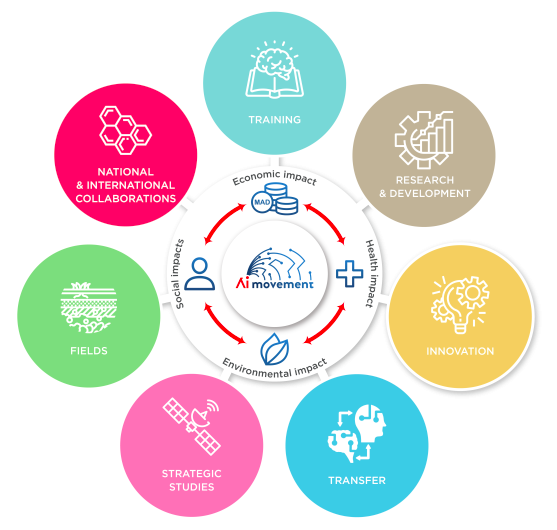
\includegraphics[width=0.3\textwidth]{images_pfe/Screenshot from 2024-06-08 18-57-32.png}
  \caption{Pillars of Ai movement.}
\end{figure}
\FloatBarrier

Structured around several pillars, the \textbf{Ai movement's initiatives} aim to:

\begin{enumerate}
    \item Develop an attractive ecosystem by fostering international collaborations and nurturing local talent.
    \item Advocate for a field-oriented approach to drive societal acceptance and understanding of AI transformations.
    \item Offer inclusive training programs tailored to various age groups and skill levels.
    \item Integrate theoretical research with practical applications to facilitate innovation and industrial transfer.
    \item Conduct strategic studies to anticipate and manage the geopolitical implications of AI advancements.

\end{enumerate}




 \section{Program Offerings}

The Ai movement offers a range of programs tailored to different aspects of artificial intelligence. A central component of our academic offerings is the \textbf{Executive Master in AI Governance and Practice}. This program is composed of the following four stackable certificates, which can be taken individually to gain specific skills or completed together to earn the full Master's degree:

\begin{itemize}
    \item \textbf{C1: AI Foundations Certificate}: Gain knowledge about AI foundations and explore the potential of machine learning in various fields.
    \item \textbf{C2: AI Application Certificate}: Explore the full potential of specific AI architectures for multiple industry applications to develop a strategic understanding of AI.
    \item \textbf{C3: AI Governance Certificate}: Learn about the latest regulations in AI and data management, as well as best practices for responsible and ethical AI.
    \item \textbf{C4: AI Transformation Certificate}: Acquire skills to manage complex AI projects and lead successful AI transformations within organizations.
\end{itemize}

In addition to the Executive Master, the Ai movement is dedicated to fostering inclusivity and early education through two flagship initiatives:

\begin{itemize}
    \item \textbf{African Women in Tech and AI Program}: This initiative supports African women in technological innovation and artificial intelligence, aligning with UNESCO's Operational Strategy for Priority Africa 2022-2029. It empowers cohorts of women to develop and lead impactful projects.
    \item \textbf{AI Master Junior Program:} An exciting initiative designed for children aged 10 to 14, this program introduces the world of AI through interactive, hands-on activities that explore its applications in daily life.
\end{itemize}


\section{Project Framework}

Multi-agent systems composed of UAVs and Unmanned Ground Vehicles (UGVs) are becoming increasingly relevant for real-world tasks such as surveillance, search and rescue, and environment monitoring. However, these agents often operate in GPS-denied or visually occluded environments that restrict their ability to observe the full state of the environment. This project explores how to improve agent coordination and decision-making in such partially observable settings using a \textbf{Masked Auto-Encoder (MAE)}.

Inspired by the effectiveness of MAEs in computer vision and NLP, this work integrates a transformer-based MAE within a Multi-Agent Reinforcement Learning (MARL) framework. The MAE reconstructs masked portions of the input, enabling agents to infer missing environmental features and form richer internal state representations.

The project is built on benchmark environments such as SMAC and SMACv2, simulating complex interactions among multiple agents. Several smart masking strategies are investigated, including random masking and TD-error-based masking. The resulting architecture is evaluated for its ability to enhance sample efficiency, coordination, and task performance.



\subsection{Context: Drone Coordination in Partially Observable Environments}
In GPS-denied or sensor-limited environments such as underground tunnels, forests, and urban disaster zones, UAVs must rely on onboard sensors like LiDAR, RGB cameras, and IMUs. These sensors can fail or provide noisy data, leading to partial observability. Swarms of UAVs must coordinate using local observations while maintaining situational awareness and achieving global objectives.

This research addresses the challenge by enabling each agent to learn latent representations that fill in missing inputs through an MAE trained in a self-supervised manner. These enhanced representations help agents to:
\begin{itemize}
\item Improve local and global awareness despite limited perception.
\item Maintain decentralized coordination in the absence of centralized communication.
\item Make informed decisions with incomplete or corrupted input.
\end{itemize}
\subsection{Objectives of the Project}
This internship project aims to achieve the following goals:
\begin{itemize}
\item Design and implement a masked auto-encoder module that can be integrated with popular MARL algorithms.
\item Explore the impact of different masking strategies (random, TD-error) on training performance.
\item Evaluate the framework in partially observable MARL benchmarks like SMAC and SMACv2.
\item Propose a masking strategy that adapts to agent learning difficulty and environmental complexity.
\item Demonstrate the benefits of the approach through ablation studies and performance comparison with baseline methods.
\end{itemize}

\subsection{Use Case Scenarios }
The project is grounded in real-world inspired scenarios where MARL agents must operate with limited or unreliable perception. The following are the primary use cases guiding this research:

\begin{itemize}
\item \textbf{GPS-Denied Navigation:} In scenarios where GPS is blocked or jammed (e.g., tunnels, urban warfare zones, or indoor operations), drones must rely solely on onboard sensors like LiDAR, RGB cameras, IMUs, and stereo cameras. The AI-based sensor fusion, enhanced by MAE, allows agents to infer location and environmental structure despite missing data.
\item \textbf{Disaster Response:} During post-disaster search and rescue operations, communication may be unstable or absent. UAVs and UGVs deployed in swarms can collaborate to explore hazardous zones, map the terrain, and locate survivors. MAE-enhanced agents help in real-time decision-making based on partial views.
\item \textbf{Autonomous Agriculture:} Swarms of drones can monitor crop health or perform coordinated tasks like pesticide dispersion or harvesting, even when individual sensors fail or encounter occlusions due to vegetation. MAEs help reconstruct consistent representations for collective task execution.
\item \textbf{Military Reconnaissance:} In hostile terrain, drone swarms can perform cooperative surveillance without relying on central control or full visibility. The masked encoding framework improves the agents' ability to maintain situational awareness even when some drones are lost or obstructed.
\item \textbf{Collaborative Exploration and Mapping:} UAV-UGV hybrid swarms can be deployed for 3D terrain reconstruction. While UAVs provide a top-down perspective, UGVs can access and report from ground level. MAEs facilitate alignment of partial, heterogeneous views into unified maps.
\end{itemize}

\subsection{Project Timeline and Work Plan}

To effectively manage the scope of this project, a structured work plan was developed, spanning a six-month period. The timeline, illustrated by the Gantt chart in Figure~\ref{fig:gantt}, outlines the major phases of the research and development process. The project began with a foundational learning period dedicated to reinforcement learning principles, followed by a thorough review of the project context and the state-of-the-art. Subsequent months were allocated to the technical implementation, beginning with the baseline setup and followed by the development of our core contribution, the LI-MA2E framework. The final two months were dedicated to intensive training, evaluation, results analysis, and the final documentation and writing of this thesis.

\begin{figure}[H]
    \centering
    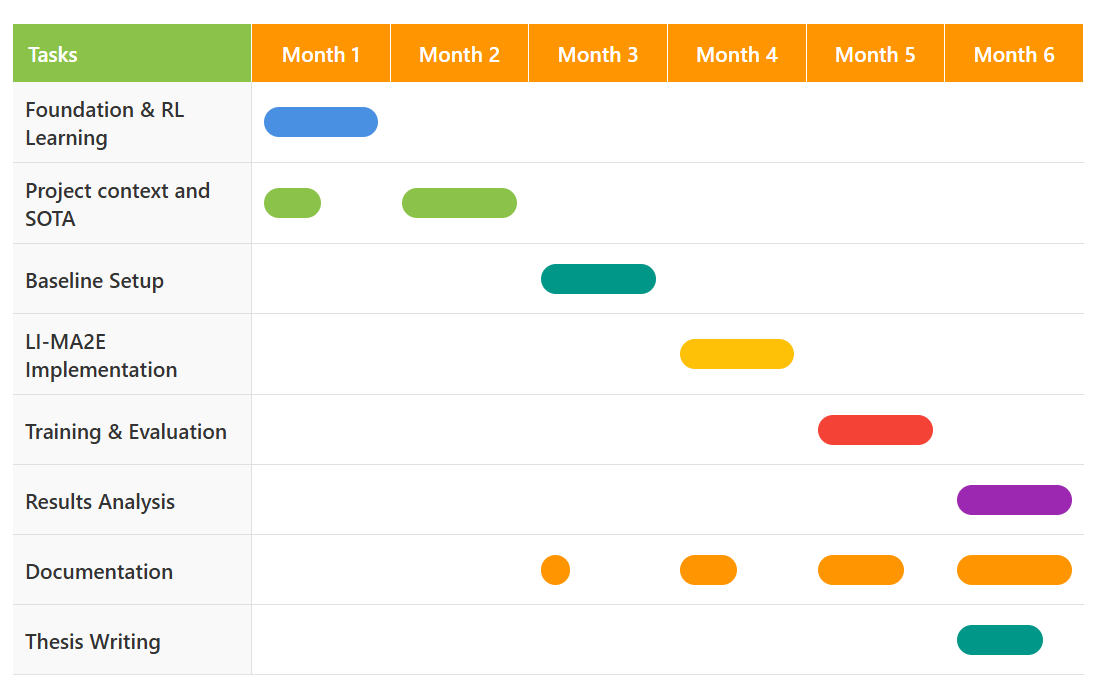
\includegraphics[width=0.7\textwidth]{images_pfe/gant.png}
    \caption{Gantt chart illustrating the project timeline and the distribution of key tasks over a six-month period.}
    \label{fig:gantt}
\end{figure}
\section*{Conclusion}
This chapter provided an overview of Mohammed VI Polytechnic University and its pioneering role in advancing artificial intelligence in Morocco and across Africa through the Ai movement center. UM6P is committed to fostering research, innovation, and sustainable development, positioning itself as a leading institution in these fields. The Ai movement, as a UNESCO Category II center, exemplifies this commitment by promoting ethical and responsible AI solutions, building local and regional expertise, and driving impactful projects across various sectors.

Our project, \textit{Enhancing Multi-Agent Reinforcement Learning under
Partial Observability via Learning-Informed Masking ($LI-MA^{2}E$)}, aligns with these objectives by proposing a novel representation learning approach based on masked auto-encoding. By strategically masking parts of agent observations and reconstructing them, our method enhances the agents' ability to act under partial observability. This contributes to more efficient training and improved coordination among agents, particularly in decentralized UAV systems operating with limited communication and incomplete environmental awareness.

The main objective of this project is to improve multi-agent learning under partial observability by developing a masking strategy that selectively focuses on less informative or poorly learning agents. This enables the model to learn richer, more generalizable representations, ultimately leading to more robust cooperative behavior in complex environments.


% In the next chapter, we present the mathematical background of the project. As well as important mathematical theories and key points, such as the Bellman Optimality equations. We also introduce Reinforcement Learning as an important paradigm in Machine Learning, in addition to the principles of Reward Shaping and Reward Reshaping.

% This section outlines the motivation and structure of our research project on addressing partial observability in MARL using MAE. By reconstructing occluded or missing information through self-supervised learning, agents become more robust and capable in complex environments. This sets the stage for subsequent chapters that detail the methodology, experimental setup, and evaluation metrics.


\chapter{Foundations of Multi-Agent Reinforcement Learning}

\section*{Introduction}
Multi-agent reinforcement learning (MARL) is, in essence, reinforcement learning (RL) applied to multi-agent game models to learn optimal policies for the agents. Thus, MARL is deeply rooted in both RL theory and game theory. This chapter provides the necessary theoretical background, starting with the foundational principles of single-agent RL before extending them to the multi-agent domain.

\section{Single-Agent Reinforcement Learning}
To understand how multiple agents learn and interact, we must first understand how a single agent learns. This section introduces the theory and algorithms of RL when there is only a single agent for which we want to learn an optimal policy. We will begin by providing a general definition of RL, following which we will introduce the Markov decision process (MDP) as the foundational model used in RL to represent single-agent decision processes. Based on the MDP model, we will define basic concepts such as expected returns, optimal policies, value functions, and Bellman equations. Most of the MARL algorithms introduced later in this chapter build on these concepts and essentially extend them to multi-agent game models.
\begin{figure}[!ht]
    \centering
    % This is a placeholder for your figure. 
     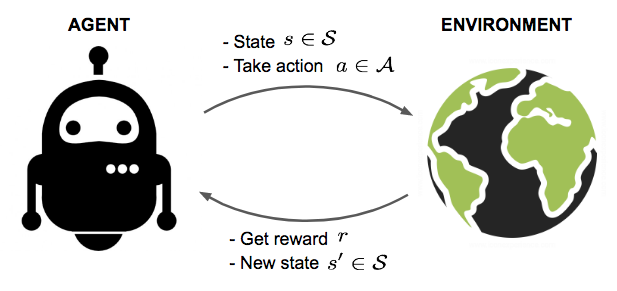
\includegraphics[width=0.48\textwidth]{img_pfe/RL_illustration.png}
    % \fbox{\rule{0pt}{4in} \rule{0.9\linewidth}{0pt}} 
    \caption{An agent interacts with the environment, trying to take smart actions to maximize cumulative rewards.}
    \label{fig:rl}
\end{figure}

\subsection*{General Definition of Reinforcement Learning}
We begin by providing a general definition of reinforcement learning:
\begin{quote}
    \textit{Reinforcement learning algorithms learn solutions for sequential decision processes via repeated interaction with an environment.} 
\end{quote}
This definition raises three main questions:
\begin{enumerate}
    \item What is a sequential decision process?
    \item What is a solution to the process?
    \item What is learning via repeated interaction?
\end{enumerate}

A sequential decision process is defined by an agent that makes decisions over multiple time steps within an environment to achieve a specified goal. In each time step, the agent receives an observation from the environment and chooses an action. Given the chosen action, the environment may change its state according to some transition dynamics and send a scalar reward signal to the agent. This fundamental interaction is often visualized as the RL loop.
\begin{figure}[h!]
\centering

 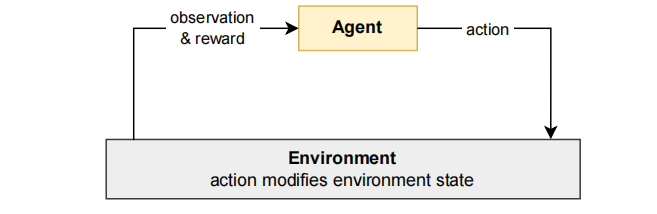
\includegraphics[width=0.8\textwidth]{img_pfe/rl_loop.PNG}
\caption{Basic reinforcement learning loop for a single-agent system.}
\label{fig:rl_loop}
\end{figure}



A solution to the decision process is an optimal decision policy for the agent, which chooses actions in each state to achieve some specified learning objective. Typically, the learning objective is to maximize the expected return for the agent in each possible state. The return is defined as the sum of rewards received over time.

Finally, RL algorithms learn via repeated interaction by trying different actions in different states and observing the outcomes. This method is often described as “trial and error.” A central problem in this learning process is the exploration-exploitation dilemma: how to balance exploring the outcomes of different actions versus sticking with (exploiting) actions that are currently believed to be best.

RL is a distinct type of machine learning. It is not supervised learning, because reward signals do not directly tell the agent which action to take. It also differs from unsupervised learning because the rewards, while not a supervised signal, act as feedback from which to learn an optimal policy. In the following sections, we will formally define these concepts within the framework of the Markov decision process.

\subsection*{Markov Decision Processes (MDPs)}
The standard model used in RL to formalize the sequential decision process is the Markov decision process.

\begin{definition}[Markov decision process]
A finite MDP consists of:
\begin{itemize}
    \item A finite set of states $\mathcal{S}$
    \item A finite set of actions $\mathcal{A}$
    \item A reward function $R: \mathcal{S} \times \mathcal{A} \times\mathcal{S} \rightarrow \mathbb{R}$
    \item A state transition probability function $T: \mathcal{S} \times \mathcal{A} \times \mathcal{S} \rightarrow [0,1]$
    \item An initial state distribution $\mu: \mathcal{S} \rightarrow [0,1]$
\end{itemize}
\end{definition}

At each time step $t$, the agent observes the current state $s_t \in \mathcal{S}$ and chooses an action $a_t \in \mathcal{A}$ according to its policy, $\pi(a_t | s_t)$. The MDP then transitions to a next state $s_{t+1}$ with probability $T(s_{t+1} | s_t, a_t)$, and the agent receives a reward $r_t = R(s_t, a_t, s_{t+1})$. This process continues until a terminal state is reached.

The term “Markov” comes from the Markov property, which states that the future is conditionally independent of the past, given the present state and action:
$$
\Pr(s_{t+1}, r_t | s_t, a_t, s_{t-1}, a_{t-1}, \dots, s_0, a_0) = \Pr(s_{t+1}, r_t | s_t, a_t)
$$

This means the current state provides all necessary information to make an optimal decision. The most common assumption in RL is that the dynamics of the MDP (the transition and reward functions) are a priori unknown to the agent.

An important special case of the MDP is the Partially Observable Markov Decision Process (POMDP), where the agent receives an observation $o_t$ rather than the true state $s_t$. POMDPs are a special case of the multi-agent models we will introduce later.

\subsection*{Expected Discounted Returns and Optimal Policies}
We have defined the MDP as a model of the decision process, but we must also define the learning objective. The most common objective is maximizing the expected discounted return.

Given that an episode may run for a long time or even indefinitely, future rewards are typically discounted by a factor $\gamma \in [0, 1)$. The discounted return is defined as:
\begin{equation}
G_t = \sum_{k=0}^{\infty} \gamma^k r_{t+k}
\end{equation}

The discount factor ensures that the sum of rewards is finite.

\subsection*{Value Functions and the Bellman Equation}
The Markov property of the decision process allows us to define the expected return on a state-by-state basis. This gives rise to the concept of value functions, which are fundamental to Reinforcement Learning. They estimate how good it is to be in a particular state, or to take a particular action in a state.

First, we can express the discounted return, $G_t$, in a recursive form:
\begin{equation}
    G_t = r_t + \gamma r_{t+1} + \gamma^2 r_{t+2} + \cdots = r_t + \gamma G_{t+1}
\end{equation}

Given a policy $\pi$, which specifies the probability $\pi(a|s)$ of taking action $a$ in state $s$, we can define two types of value functions:

\paragraph{The State-Value Function ($V^\pi$):}
This function gives the expected return when starting in state $s$ and following policy $\pi$ thereafter. It is defined as:
\begin{equation}
    V^\pi(s) = \mathbb{E}_\pi[G_t | S_t = s]
\end{equation}

The state-value function adheres to a recursive relationship known as the Bellman equation:
\begin{equation}
    V^\pi(s) = \sum_{a \in \mathcal{A}} \pi(a|s) \sum_{s' \in \mathcal{S}} P(s'|s,a)[R(s,a,s') + \gamma V^\pi(s')]
\end{equation}

For a finite state space, this equation forms a system of linear equations whose unique solution is the value function $V^\pi$.

\paragraph{The Action-Value Function ($Q^\pi$):}
This function gives the expected return after taking a specific action $a$ in state $s$ and then following policy $\pi$. It is defined as:
\begin{equation}
    Q^\pi(s,a) = \mathbb{E}_\pi[G_t | S_t = s, A_t = a]
\end{equation}

Similar to the state-value function, $Q^\pi$ satisfies its own Bellman equation:
\begin{equation}
    Q^\pi(s,a) = \sum_{s' \in \mathcal{S}} P(s'|s,a)[R(s,a,s') + \gamma V^\pi(s')]
\end{equation}

By substituting $V^\pi(s') = \sum_{a' \in \mathcal{A}} \pi(a'|s') Q^\pi(s',a')$, we can express the Bellman equation for $Q^\pi$ solely in terms of action-values:
\begin{equation}
    Q^\pi(s,a) = \sum_{s' \in \mathcal{S}} P(s'|s,a) \left[ R(s,a,s') + \gamma \sum_{a' \in \mathcal{A}} \pi(a'|s') Q^\pi(s',a') \right]
\end{equation}

\subsection*{Optimal Value Functions and Policies}
The ultimate goal in an MDP is to find an optimal policy, denoted $\pi^*$, that maximizes the expected return. A policy is considered optimal if its expected return is greater than or equal to that of all other policies for all states. Such a policy shares a unique optimal value function.

The optimal state-value function, $V^*(s)$, and optimal action-value function, $Q^*(s,a)$, are defined as:
\begin{align}
    V^*(s) &= \max_{\pi} V^\pi(s), \quad \forall s \in \mathcal{S} \\
    Q^*(s,a) &= \max_{\pi} Q^\pi(s,a), \quad \forall s \in \mathcal{S}, a \in \mathcal{A}
\end{align}

These optimal value functions satisfy a special set of recursive equations called the Bellman optimality equations. Unlike the standard Bellman equations, these are non-linear due to the maximization operator.

The Bellman optimality equation for $V^*$ is:
\begin{equation}
    V^*(s) = \max_{a \in \mathcal{A}} \sum_{s' \in \mathcal{S}} P(s'|s,a) [R(s,a,s') + \gamma V^*(s')]
\end{equation}

And for $Q^*$:
\begin{equation}
    Q^*(s,a) = \sum_{s' \in \mathcal{S}} P(s'|s,a) \left[ R(s,a,s') + \gamma \max_{a' \in \mathcal{A}} Q^*(s',a') \right]
\end{equation}

Solving this system of non-linear equations provides the optimal action-value function, $Q^*$. Once $Q^*$ is known, the optimal policy $\pi^*$ can be derived by deterministically selecting the action with the maximum value in each state:
\begin{equation}
    \pi^*(s) = \arg\max_{a \in \mathcal{A}} Q^*(s,a)
\end{equation}

While the optimal value function is unique for a given \textit{MDP}, there can be multiple optimal policies that achieve this same maximum value. The existence of a solution to the Bellman optimality equation guarantees that there is always at least one deterministic optimal policy. The methods for solving these equations, such as dynamic programming and temporal-difference learning, are central to finding solutions for reinforcement learning problems.
% \subsection{Methods for Solving MDPs}
% Now that we have formally defined the components of an MDP and the objective of finding an optimal policy, we turn our attention to the algorithms designed to solve for $V^*$ and $\pi^*$. These methods provide the computational foundation for reinforcement learning. We begin with methods that require a complete model of the environment.
%---- old dynamic --------
% \subsection*{Dynamic Programming}
% Dynamic Programming (DP) is a collection of algorithms that compute optimal policies given a perfect model of an MDP, meaning the transition probabilities $T(s'|s, a)$ and the reward function, $R(s, a,s')$, must be fully known.

% DP is foundational because it turns the Bellman equations into iterative update rules to find optimal value functions. Key DP methods like Policy Iteration and Value Iteration introduce the concept of bootstrapping—updating a state's value estimate based on the values of its successor states, which is a core property of many RL algorithms.

% \paragraph{Policy Iteration}
% Policy iteration finds the optimal policy $\pi^*$ by alternating between two steps: policy evaluation and policy improvement. It starts with an initial policy $\pi_0$ and refines it until it converges.

% The process follows this pattern:
% $$ \pi_0 \xrightarrow{\text{evaluate}} V^{\pi_0} \xrightarrow{\text{improve}} \pi_1 \xrightarrow{\text{evaluate}} V^{\pi_1} \xrightarrow{\text{improve}} \pi_2 \rightarrow \dots \rightarrow \pi^* $$

% \begin{enumerate}
%     \item \textbf{Policy Evaluation:} For the current policy $\pi$, we compute the state-value function $V^\pi$. This is done by iteratively applying the Bellman equation as an update rule, starting with an arbitrary value function $V_0$:
%     \begin{equation}
%     V_{k+1}(s) \leftarrow \sum_{a \in A} \pi(a|s) \sum_{s' \in S} T(s'|s,a) [R(s,a,s') + \gamma V_k(s')] 
%     \end{equation}
%     This process is guaranteed to converge to the true value function $V^\pi$. This is because the Bellman operator is a $\gamma$-contraction mapping, which, by the Banach fixed-point theorem, ensures convergence to a unique fixed point.

%     \item \textbf{Policy Improvement:} Once $V^\pi$ is computed, the policy is improved by making it greedy with respect to the value function. For each state, the new policy $\pi'$ greedily selects the best action:

%     \begin{equation}
%     \pi^{'}(s)  \leftarrow \arg\max_{a \in A} \sum_{s' \in S} T(s'|s,a) [R(s,a,s') + \gamma V^\pi(s')]
%    \end{equation}
%     Thanks to the policy improvement theorem, this new policy $\pi'$ is guaranteed to be as good as, or better than, $\pi$.
% \end{enumerate}

% These two steps are repeated until the policy is stable (i.e., $\pi' = \pi$), which indicates that the policy is optimal and satisfies the Bellman optimality equation.

% \paragraph{Value Iteration}
% This method merges policy evaluation and improvement into a single step. Starting with an initial value function $V_0(s)$, it repeatedly updates it using the Bellman optimality equation:
% $$ V_{k+1}(s) \leftarrow \max_{a \in A} \sum_{s' \in S} T(s'|s,a) [R(s,a,s') + \gamma V_k(s')] $$
% The process continues until the value changes are below a threshold. The optimal policy is then extracted by selecting the action that maximizes the expected return in each state:
% $$ \pi^*(s) \leftarrow \arg\max_{a \in A} \sum_{s' \in S} T(s'|s,a) [R(s,a,s') + \gamma V^*(s')] $$
% Value iteration is often faster than policy iteration since it avoids full evaluation of intermediate policies.
% \subsection*{Temporal-Difference Learning}
% While Dynamic Programming provides a solid foundation for solving MDPs, its requirement of a complete model of the environment ($T$ and $R$) is a significant limitation. In most real-world scenarios, the agent does not know the underlying dynamics. Temporal-Difference (TD) learning is a central concept in RL that allows an agent to learn directly from raw experience, making it a model-free approach.

% Like DP, TD learning uses bootstrapping to update value estimates based on other learned estimates. However, instead of sweeping through the entire state space, it learns from incomplete episodes, updating its knowledge after each time step. The agent interacts with the environment by executing an action $a_t$ from a state $s_t$, receiving a reward $r_t$, and observing the next state $s_{t+1}$. This experience tuple, $(s_t, a_t, r_t, s_{t+1})$, is used to update the action-value function, $Q(s_t, a_t)$.

% The general update rule for TD learning is:
% $$ Q(s_t, a_t) \leftarrow Q(s_t, a_t) + \alpha[\text{TD Target} - Q(s_t, a_t)] $$
% Here, $\ alpha\in [0,1]$ is the learning rate, and the TD Target is an estimate of the return that the agent aims to achieve. The term $\text{TD Target} - Q(s_t, a_t)$ is known as the TD error. The two most fundamental TD algorithms, Sarsa and Q-learning, differ in how they define this target.

% A critical challenge in model-free learning is the exploration-exploitation dilemma. To find the optimal policy, the agent must exploit actions it knows to be good, but it must also explore other actions to discover potentially better ones. A common solution is the $\epsilon$-greedy policy, where the agent chooses the best-known action with probability $1-\epsilon$ and a random action with probability $\epsilon$. To ensure convergence, all state-action pairs must be visited, and $\epsilon$ can be gradually decreased over time.

% \paragraph{Sarsa: On-Policy TD Control}
% Sarsa is an on-policy TD algorithm, meaning it learns the value of the policy the agent is currently following (including its exploratory actions). The name Sarsa comes from the quintuple of experience it uses for its update: $(s_t, a_t, r_t, s_{t+1}, a_{t+1})$.

% The Sarsa update rule is defined by using the following TD target:
% $$ \text{TD Target} = r_t + \gamma Q(s_{t+1}, a_{t+1}) $$
% The full update rule is:
% $$ Q(s_t, a_t) \leftarrow Q(s_t, a_t) + \alpha[r_t + \gamma Q(s_{t+1}, a_{t+1}) - Q(s_t, a_t)] $$
% Crucially, the action $a_{t+1}$ is the actual action taken by the agent in the next state $s_{t+1}$ according to its current policy (e.g., the $\epsilon$-greedy policy). Because the update depends on the policy being followed, Sarsa is considered on-policy. It learns a policy that is optimal given its own exploration strategy.

% \paragraph{Q-learning: Off-Policy TD Control}
% Q-learning is an off-policy TD algorithm. This means it can learn the optimal policy $\pi^*$ even while following a different, more exploratory policy. It achieves this by defining its TD target based on the Bellman optimality equation.

% The Q-learning update rule uses a greedy target that always selects the action with the maximum possible value in the next state:
% \begin{equation}
%     \text{TD Target} = r_t + \gamma \max_{a'} Q(s_{t+1}, a')
% \end{equation}

% The full update rule is:
% \begin{equation} Q(s_t, a_t) \leftarrow Q(s_t, a_t) + \alpha[r_t + \gamma \max_{a'} Q(s_{t+1}, a') - Q(s_t, a_t)] \end{equation}
% The max operator allows Q-learning to update its Q-value for $(s_t, a_t)$ assuming the best possible action will be taken from $s_{t+1}$, regardless of which action the agent actually takes next. This separation of the learning policy (always greedy) from the behavior policy (e.g., $\epsilon$-greedy) makes Q-learning off-policy and a more direct, though sometimes less stable, approach to finding the optimal policy.
%----fin old ----
\subsection{Dynamic programming}
There are two basic families of algorithms to compute optimal policies for MDPs: dynamic programming and temporal-difference learning.
Dynamic programming requires complete knowledge of the MDP specification
and uses this knowledge to compute optimal value functions and policies. In
contrast, temporal-difference learning does not require complete knowledge
of the MDP, instead, it learns optimal value functions and policies by inter-
acting with the environment and generating experiences.

\subsubsection{Policy Iteration}

Policy iteration is an iterative algorithm used to compute the optimal policy for an MDP. It consists of two main steps: policy evaluation and policy improvement.

1. \textbf{Policy Evaluation}: Given a policy \(\pi\), we evaluate its value function \(V^\pi(s)\) by solving the following system of linear equations for all states \(s \in \mathcal{S}\):

\[
V^\pi(s) = \sum_{a \in \mathcal{A}} \pi(a|s) \sum_{s' \in \mathcal{S}} P(s'|s, a) \left[ R(s, a, s') + \gamma V^\pi(s') \right]
\]

Where:
\begin{itemize}
    \item \(\pi(a|s)\) is the probability of taking action \(a\) in state \(s\) under policy \(\pi\),
    \item \(P(s'|s, a)\) is the transition probability from state \(s\) to state \(s'\) given action \(a\),
    \item \(R(s, a, s')\) is the reward received when transitioning from state \(s\) to state \(s'\) given action \(a\),
    \item \(\gamma\) is the discount factor.
\end{itemize}

2. \textbf{Policy Improvement}: Using the value function \(V^\pi(s)\) computed in the policy evaluation step, we improve the policy by choosing actions that maximize the expected value. The improved policy \(\pi'\) is given by:

\[
\pi'(s) = \arg\max_{a \in \mathcal{A}} \sum_{s' \in \mathcal{S}} P(s'|s, a) \left[ R(s, a, s') + \gamma V^\pi(s') \right]
\]

The policy iteration algorithm alternates between these two steps until the policy converges to the optimal policy \(\pi^*\).

\subsubsection{Value Iteration}

Value iteration is another dynamic programming algorithm used to find the optimal policy by iteratively updating the value function. Unlike policy iteration, value iteration combines policy evaluation and policy improvement into a single step. The Bellman equation for value iteration is given by:

\[
V_{k+1}(s) = \max_{a \in \mathcal{A}} \sum_{s' \in \mathcal{S}} P(s'|s, a) \left[ R(s, a, s') + \gamma V_k(s') \right]
\]

where \(V_k(s)\) is the value function at iteration \(k\).

Once the value function \(V(s)\) has converged, the optimal policy \(\pi^*\) can be extracted as:

\[
\pi^*(s) = \arg\max_{a \in \mathcal{A}} \sum_{s' \in \mathcal{S}} P(s'|s, a) \left[ R(s, a, s') + \gamma V(s') \right]
\]

Both policy iteration and value iteration are powerful methods in dynamic programming for solving MDPs and computing optimal policies. Both their algorithms can be found in the Annex. In the next section, we dig deep into the Bellman equations for states and action functions that are the foundation of the policy iteration and value iteration algorithms.




\subsection{Bellman's Optimality equations}
There are two key Bellman equations used in dynamic programming for MDPs: the state value function and the state-action value function. These equations provide the foundation for computing optimal policies by recursively breaking down the expected returns.


\begin{itemize}
    \item \textbf{State Value function for policy $\pi$:} The value of a state is the expected return starting from that state; it depends on the agent’s policy: 
    \begin{equation}
    V^{\pi} (s) = E_{\pi} \{ R_t | s_t = s \} = E_{\pi} \{ \sum _{k=0} ^{\infty} \gamma ^{k} r_{t+k+1} | s_t=s \}
    \end{equation}
    \item \textbf{Action Value function for policy $\pi$}: The value of taking an action in a state under policy $\pi$ is the expected return starting from that state, taking that action, and thereafter following $\pi$:
    \begin{equation}
        Q^{\pi} (s,a) = E_{\pi} \{ R_t | s_t = s, a_t =a \} = E_{\pi} \{ \sum _{k=0} ^{\infty} \gamma ^{k} r_{t+k+1} | s_t=s, a_t =a \}
    \end{equation}
\end{itemize}

We can calculate the reward as: 
\begin{equation}
\begin{aligned}
     R_t = &  r_{t+1} + \gamma r_{t+2} + \gamma ^{2} r_{t+3} + \gamma ^{3} r_{t+4} + \cdots
     \\     R_t = & r_{t+1} + \gamma R_{t+1}
\end{aligned}
\end{equation}
\vspace*{0.1cm}

So the \textbf{state-value function} and the \textbf{Action-value function} become: 
\begin{equation}
\begin{aligned}
        V^{\pi} (s) = & E_{\pi} \{ R_t | s_t = s \} = E_{\pi} \{ r_{t+1} + \gamma V^{\pi} (s_{t+1}) | s_i = s \} 
        \\     Q^{\pi} (s,a) = E_{\pi} \{ R_t & | s_t = s, a_t=a \} = E_{\pi} \{ r_{t+1} + \gamma V^{\pi} (s_{t+1}) | s_i = s, a_t=a \}
\end{aligned}
\end{equation}
\vspace*{0.1cm}

In a \textbf{deterministic} environment, the state-value function and the action-value function are defined as: 

\begin{equation}
\begin{aligned}
        V^{\pi} (s) & =  r(s, \pi (s) , s') + \gamma V^{\pi} (s')
  \\           Q^{\pi} (s,a) & =  r(s, a , s') + \gamma V^{\pi} (s')
\end{aligned}
\end{equation}


The Bellman equations provide a way to decompose the problem of finding optimal policies into simpler, recursive relationships involving value functions. However, in practice, several challenges necessitate the use of estimations (approximations) rather than exact calculations. We use \textbf{TD errors }to quantify the discrepancy between the predicted and actual outcomes as computed by the Bellman equations:

\begin{equation}
    \begin{aligned}
        TDerror(s) = & \ V^{\pi} (s) - \sum _{s'} T(s, \pi (s) , s') [ r(s, \pi (s) , s') + \gamma V^{\pi} (s')]
        \\
        TDerror(s,a) = & \ Q^{\pi} (s,a) - \sum _{s'} T(s, a , s') [ r(s, a , s') + \gamma V^{\pi} (s')]
    \end{aligned}
\end{equation}

Estimating these errors helps in adjusting the value functions \( V^{\pi}(s) \) and \( Q^{\pi}(s,a) \) towards more accurate representations of the true values.


The goal is for the agent (or agents) to find the \textbf{optimal policy} $\pi ^{*}$ using the \textbf{Bellman Backup} that we will go into in the next section. Optimal policies are the greedy policies with respect to the functions $V^{*}$ or $Q^{*}$. And we say \textbf{Bellman's Optimality equations} to talk about the state-value function, as well as the action-value function in the case of learning the optimal policy $\pi ^{*}$.
\begin{figure}[H]
    \centering
    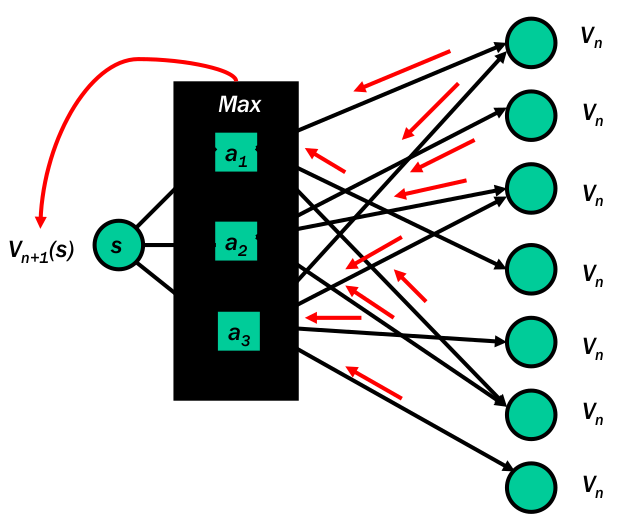
\includegraphics[width=0.3\linewidth]{images_pfe/Screenshot from 2024-06-14 17-08-41.png}
    \caption{Bellman Backup}
    \label{fig:Bellman-Backup}
\end{figure}
\section{Deep Reinforcement Learning}
\subsection{Reinforcement Learning}
Reinforcement Learning can be classified into two paradigms: model-based and model-free. In the case of model-based approaches, agents attempt to learn the transition function $T$, which can then be used when making action selections. By contrast, in the model-free approach, knowledge of T is not a requirement. Model-free learners instead sample
The underlying MDP is used to gain knowledge about the unknown model, in the form of
of value function estimates (Q values). These estimates represent the expected utility of each
state-action pair, which aids an agent in deciding which action is most desirable to select when in
a certain state.

An RL agent must find a balance between exploiting known good actions and exploring
the consequences of new actions to maximise the reward received during its lifetime. Two algorithms that are commonly used to manage the exploration-exploitation trade-off are
$\epsilon - \text{greedy}$ and softmax. The $\epsilon - \text{greedy}$ strategy selects the action with the highest expected value with probability $1 − \epsilon $, or a randomly selected action with the remaining probability $\epsilon $.


\subsection{Deep Q-Network}
\textbf{Q-learning} \parencite{Watkins} is one of the most commonly used RL algorithms. It is a model-free algorithm that has been shown to converge to the optimum action-values for an MDP with probability 1, so long as all actions in all states are sampled infinitely often and the
action-values are represented discretely. In practice, Q-learning will
learn good policies provided a sufficient number of samples are obtained for each state-action
pair. Agents implementing Q-learning update their Q values according to the following update rule:
\begin{equation}
    Q(s,a) \leftarrow Q(s,a) + \alpha [ r + \gamma max_{a'} Q(s',a') - Q(s,a)]
\end{equation}

Q values may be initialized in a number of different ways. The simplest method is to set the values for all state-action pairs to zero, i.e., \( \forall s, a \quad Q(s, a) = 0 \). Value function estimates may also be initialized using random values, \textbf{optimistic values}, or pessimistic values. \textbf{Optimistic initialization} sets the value for each state-action pair to the maximum possible reward; conversely, pessimistic initialization sets the value for each state-action pair to the minimum possible reward. The theoretical guarantees of Q-learning hold with any arbitrary initial Q values; therefore, the optimal policy for an MDP can be learned with any initial value function estimates.


Tabular representations are the simplest way to store value function estimates, where each state-action pair has a discrete \( Q \) value associated with it. When \( Q \) values are represented discretely, each additional feature tracked in the state leads to an exponential growth in the number of state-action pair values that must be stored \cite{Sutton1998}. This problem is commonly referred to in the literature as the \textbf{“curse of dimensionality”,} a term originally coined by Bellman \parencite{Bellman1957}. In simple environments, this is rarely an issue, but it may lead to an intractable problem in real-world applications due to memory or computational constraints. Learning over a large state-action space is possible, but it may take an unacceptably long time to learn useful policies. Alternatively, function approximation may be used to generalize across states and/or actions, whereby a \( Q \) function is used to store and retrieve estimates of the utility of state-action pairs. Function approximation, therefore, offers a way to mitigate against the state-action space explosion and is an active area of research in RL. Tile coding is one of the simplest forms of function approximation, where one tile represents multiple states or state-action pairs.


Neural Networks are also commonly used to implement Q functions, one of the most famous examples being Tesauro’s application of RL to backgammon (Tesauro 1994). It has been established that applied Deep Neural Networks can be a function approximation method; this emerging paradigm is known as \textbf{Deep Reinforcement Learning}. Deep RL has achieved human-level performance (or above) on complex tasks such as playing Atari games (Mnih et al. 2015) and playing the board game Go (Silver et al. 2016). Figure 2.1 shows a schematic of a DQN implemented in a Markov Decision Process. 

Tabular representations are used exclusively throughout this thesis for several reasons, including the fact that Q values must be represented discretely to preserve the theoretical guarantees offered by Q-learning \parencite{Watkins}. Although \textbf{reward shaping} could be applied in cases where function approximation is used, its use presents difficulties concerning developing theoretical guarantees for the techniques considered (Potential-based Reward Shaping and difference rewards).

\begin{figure}[hbt!]
  \centering
  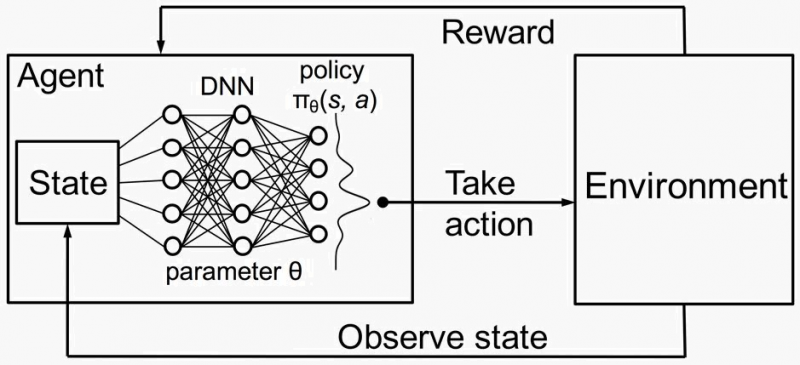
\includegraphics[width=0.5\textwidth]{images_pfe/1_ZZJ2FJFDNB9W-kdA2CfmTQ.png}
  \caption{DQN implementation in an MDP}
  \label{fig:dqn_mdp}
\end{figure}
\FloatBarrier

\textbf{Deep Q-Networks} (DQNs) build upon the principles of the Bellman Optimality equations, which are fundamental in RL. These equations describe how optimal value functions satisfy a recursive relationship, guiding the agent to maximize expected rewards over time. In practice, iterative methods like the Bellman backup are employed, where the equality in the Bellman Optimality equation is replaced with an update assignment:
\begin{equation}
    U_{i+1}(s) \leftarrow R(s) + \gamma \max_{a} \sum_{s'} T(s, a, s') U_i(s')
\end{equation}
This update, known as the \textbf{Bellman backup} (shown in \ref{fig: Bellman-Backup}), iteratively refines the estimate \( U_i(s) \) of the utility of state \( s \). The process continues until convergence, where \( U_i(s) \) approaches \( U^*(s) \), the optimal utility function, as \( i \) increases. DQNs leverage these principles to approximate the optimal action-value function \( Q^*(s, a) \) efficiently, using deep neural networks to approximate \( U_i(s) \) across large state spaces, thereby enabling complex decision-making in real-world applications of RL.

\subsection{From a Stochastic setting to a unique action}
An agent in a grid is always facing multiple choices when it comes to the actions it can take at any time step $t$, if we suppose the action space is $A=\{ 0,1,2,3,4 \} $, with: 
\begin{itemize}
    \item $0$: the agent stays in its previous state and does not move.
    \item $1$: the agent moves to the case that is adjacent to its right
    \item $2$: the agent moves to the case that is adjacent to its left
    \item $3$: the agent goes up
    \item $4$: the agent goes down
\end{itemize}
The current state of each agent is fed to the DQN as input. The information it holds gets encoded in the weights of the neurons of the DQN, and based on the current weights of the neural network, values are assigned to each of the actions $\{ 0,1,2,3,4 \} $. The final action that the agent chooses is through the \textbf{Maximum Expected Utility Principle:} The agent simply chooses the action that maximizes the expected utility of the subsequent state: 
\begin{equation}
    \pi (s) \in argmax _{a} \sum _{s'} T(s,a,s') U(s')
\end{equation}


\begin{figure}[hbt!]
  \centering
  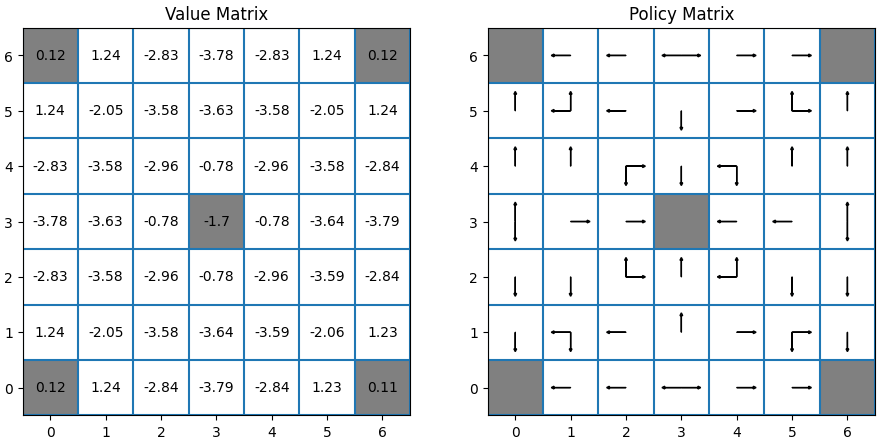
\includegraphics[width=0.7\textwidth]{images_pfe/1_tT9D_A8yJ0xkoul8e4H3Eg.png}
  \caption{Value Matrix and Policy Matrix for a Stochastic Setting (grid example).}
  \label{fig:value_policy_matrix_grid}
\end{figure}
\FloatBarrier

As shown in the figure above (\ref{fig:value_policy_matrix_grid}), the value of a state $s$ or the payoff of being in that state is represented by a number (eg.  $ 1.24, -0.78, \cdots $). The utility of a state is the immediate reward for that
state plus the expected discounted utility of the next
state, assuming that the agent chooses the optimal
action: 

\begin{equation}
    U(s) = R(s) + \gamma max _{a} \sum _{s'} T(s,a,s') U(s')
\end{equation}
This equation is the foundation of the \textbf{Bellman Backup principle}.

The state-action pairs values, or quality of taking an action $a_i$ given that the agent is in state $s$, is learned by the neural network using a \textbf{Loss function} that allows for the current DQN to converge to the Target DQN. Before the learning of the agents starts, both networks are initialized and are updated after each time step. The target network parameters $\theta^-$ are updated less frequently than the current network parameters $\theta$ to help stabilize training by providing consistent targets for a number of time steps. In literature, this is described as "DQN following its tail".


The loss function is mathematically expressed as:
\begin{equation}
    [
L(\theta) = \mathbb{E}_{(s, a, r, s') \sim \mathcal{D}} \left[ \left( y - Q(s, a; \theta) \right)^2 \right]
]
\end{equation}

Where:

\begin{itemize}
    \item $\theta$ are the parameters of the current Q-network.
    \item $\mathcal{D}$ is the replay buffer containing tuples $(s, a, r, s')$ of states, actions, rewards, and next states.
    \item $y$ is the target Q-value, defined as:
    \[
    y = r + \gamma \max_{a'} Q(s', a'; \theta^-)
    \]
    Here:
    \begin{itemize}
        \item $r$ is the reward received after taking action $a$ in state $s$.
        \item $\gamma$ is the discount factor.
        \item $\theta^-$ are the parameters of the target Q-network (which are periodically updated to match $\theta$).
    \end{itemize}
\end{itemize}

The \textbf{Replay Buffer ($\mathcal{D}$)} stores past experiences in the form of tuples $(s, a, r, s')$. During training, mini-batches of these experiences are sampled randomly to break the correlation between consecutive experiences, improving the stability and efficiency of learning. The \textbf{Target Q-Value ($y$)} is computed using the reward $r$ received plus the discounted maximum Q-value for the next state $s'$ using the target network. This incorporates the Bellman optimality equation to ensure that the network learns to predict future rewards accurately. And the \textbf{Loss Function} $L(\theta)$ is the mean squared error between the target Q-value $y$ and the predicted Q-value $Q(s, a; \theta)$ from the current Q-network. By minimizing this loss, the parameters $\theta$ of the current Q-network are adjusted to bring the predicted Q-values closer to the target Q-values.


\section{From Single-Agent to Multi-Agent Reinforcement Learning}
The principles of single-agent RL provide the building blocks for MARL. However, when multiple learning agents interact within a shared environment, the problem's complexity increases significantly. The environment's dynamics become dependent on the joint action of all agents, and each agent's success is tied to the behavior of others. This section formally introduces the models used in MARL and highlights the fundamental challenges that arise.

\subsection{The Formalism: Stochastic Games}
The standard single-agent MDP is insufficient to model a multi-agent system. The natural extension of the MDP to the multi-agent domain is the Stochastic Game (SG), also known as a Markov Game.

\begin{definition}[Stochastic Game]
A stochastic game is a tuple $\langle \mathcal{I}, S, \{A_i\}_{i \in \mathcal{I}}, T, \{R_i\}_{i \in \mathcal{I}}, \gamma \rangle$, where:
\begin{itemize}
    \item $\mathcal{I}$ is a finite set of $n$ agents, indexed by $i=1,...,n$.
    \item $S$ is the finite set of environment states.
    \item $A_i$ is the finite set of actions available to agent $i$. The joint action space is $A = A_1 \times \dots \times A_n$.
    \item $T: S \times A \times S \to [0,1]$ is the state transition probability function, which maps a state and a joint action to a distribution over next states.
    \item $R_i: S \times A \times S \to \mathbb{R}$ is the reward function for agent $i$.
    \item $\gamma \in [0,1]$ is the discount factor.
\end{itemize}
\end{definition}

At each timestep $t$, the system is in state $s_t \in S$. Each agent $i$ chooses an action $a_{i,t} \in A_i$, forming a joint action $a_t = (a_{1,t}, ..., a_{n,t}) \in A$. The environment then transitions to a new state $s_{t+1}$ with probability $T(s_{t+1} | s_t, a_t)$, and each agent $i$ receives a reward $r_{i,t}$.

The relationship between the agents' reward functions defines the nature of the game:

\paragraph{Fully Cooperative (Common-Reward)} All agents share the same reward function ($R_i = R_j$ for all $i,j$). Their goal is to collaborate to maximize this common reward. This is the setting for your project.

\paragraph{Fully Competitive (Zero-Sum)} The sum of rewards is always zero ($\sum_{i} R_i = 0$). One agent's gain is another's loss.

\paragraph{General-Sum} The most general case with no restrictions on the rewards. This can model mixed cooperative and competitive interactions.

\subsection{Core Challenges in MARL}
Moving from an MDP to an SG introduces fundamental challenges that render single-agent RL algorithms insufficient.

\subsubsection{Non-Stationarity}
% From the perspective of a single agent $i$, the environment is no longer stationary. The transition and reward dynamics depend on the actions of all other agents. As other agents update their policies $\pi_j$, the optimal policy for agent $i$ changes. This breaks the stationary Markov assumption
% that underpins algorithms like Q-learning, as the environment appears to be a constantly "moving target."
To any single agent, the environment seems unstable or non-stationary. This is because the result of its actions depends on the choices of all other agents. Since those other agents are also learning and constantly changing their strategies, the world becomes a \textbf{moving target}. An action that was good before might become bad now, breaking the stable environment assumption that is crucial for basic algorithms like Q-learning.
\subsubsection{Multi-Agent Credit Assignment}
 This challenge compounds the standard temporal credit assignment problem. In a cooperative setting, when a team receives a shared reward, it is highly non-trivial to determine the specific contribution of each individual agent's action to the team's success.
\subsubsection{Scalability}
 The joint action space of a multi-agent system often grows exponentially with the number of agents. This "curse of dimensionality" presents a significant barrier to scaling algorithms to systems with a very large number of agents.
\subsubsection{Partial Observability}
In most realistic scenarios, agents do not have access to the full environment state $s_t$. Instead, each agent $i$ receives a private, partial observation $o_{i,t}$ which contains incomplete information about $s_t$. This brings us to the most general framework for MARL, the Partially Observable Stochastic Game (POSG). For cooperative tasks, this is more specifically referred to as a Decentralized Partially Observable Markov Decision Process (Dec-POMDP).

\begin{definition}[Dec-POMDP]
A Dec-POMDP extends the Stochastic Game with observation components:
\begin{itemize}
    \item A set of observations for each agent, $\Omega_i$.
    \item An observation function $O: S \times A \to \mathcal{P}(\Omega)$ which gives the probability of a joint observation $o_t = (o_{1,t}, ..., o_{n,t})$ after a joint action $a_{t-1}$ leads to state $s_t$.
\end{itemize}
\end{definition}

Under partial observability, an agent cannot simply map its current observation to an optimal action. It must account for the history of its past observations to infer a belief about the true state of the environment. In deep RL, this is often achieved practically by equipping agent policies with memory, for example, by using Recurrent Neural Networks (RNNs) to process sequences of observations.\parencite{ma_deep_rl_challenges_and_applications}

Our project directly tackles this challenge of learning effective policies from partial observations in a cooperative setting.

% \subsubsection{The Goal: From Equilibrium to Coordination}
\subsubsection{From Equilibrium to Coordination}
In a general-sum SG, the solution is typically a Nash Equilibrium: a joint policy where no single agent can improve its own return by unilaterally changing its policy. However, in the fully cooperative (common-reward) setting of a Dec-POMDP, the objective is simpler and more direct: find the optimal joint policy $\pi^*$ that maximizes the shared expected return for the entire team.
$$ \pi^* = \arg\max_{\pi} \mathbb{E} \left[ \sum_{t=0}^{\infty} \gamma^t R(s_t, a_t, s_{t+1}) \right] $$
Solving this cooperative problem is the primary focus of the MARL algorithms we will discuss next, particularly those built on the CTDE paradigm.




% \subsection{Centralized Training with Decentralized Execution (CTDE)}
% Given the challenges of non-stationarity and partial observability, how can agents effectively learn to cooperate? A naive approach where each agent learns independently often fails because the environment is a \textbf{moving target.} The Centralized Training with Decentralized Execution (CTDE) paradigm offers an elegant and powerful solution.

% The core idea is to leverage different information structures during the training and execution phases:
% \begin{itemize}
%     \item \textbf{Centralized Training:} During the learning phase, the algorithm can access global information---such as the observations and actions of all agents---to train the policies more effectively. This privileged information helps overcome non-stationarity and aids credit assignment.
%     \item \textbf{Decentralized Execution:} After training, the centralized component is discarded. Each agent makes decisions using only its own local action-observation history, making the policies practical for real-world deployment.
% \end{itemize}

% \paragraph{The CTDE Actor-Critic Approach}
% A common way to implement CTDE is with an actor-critic architecture.

% \begin{description}
   

%     \item[The Actors (Decentralized Policies)] Each agent $i$ has its own policy, $\pi_i$, which is its actor. The actor is decentralized, mapping the agent's local action-observation history, $h_i$, to an action:
%     $$ \text{Actor}_i : \pi_i(a_i | h_i) $$
    
%     \item[The Critic (Centralized Value Function)] A single, centralized critic is used during training to evaluate the joint actions of the team. This critic is an action-value function, $Q_{\pi}(h,a)$, that takes the joint history $h = \langle h_1, \dots, h_n \rangle$ and joint action $a$ as input.
% \end{description}
% Formally, for a given joint policy $\pi$, this centralized Q-function represents the total expected discounted reward from taking joint action $a$ in joint history $h$ and following the joint policy $\pi$ thereafter. It can be defined recursively:
% $$ Q_{\pi}(h,a) = \sum_{s \in S} P(s|h) \left( R(s,a) + \gamma \sum_{s' \in S} T(s'|s,a) \sum_{o \in \Omega} O(o|s',a) V_{\pi}(hao) \right) $$
% where $V_{\pi}(hao)$ is the value of the next joint history.

% In practice, an RL algorithm does not compute this expectation exactly. Instead, it approximates the critic's value through sampling from experiences collected during training. The goal of the centralized critic is to provide a stable and high-quality learning signal to the actors.

% During training, the agents follow their local actors to generate experience. The centralized critic evaluates this experience and guides the updates for each decentralized actor, effectively telling the team which joint behaviors lead to success. After training, the complex critic is discarded, leaving only the efficient decentralized actors for execution. This framework is the foundation for many state-of-the-art cooperative MARL algorithms.
\subsection{Centralized Training with Decentralized Execution (CTDE)}
Given the challenges of non-stationarity and partial observability, a naive approach where each agent learns independently often fails because the environment is a constantly moving target. The CTDE paradigm offers an elegant and powerful solution.

The core idea is to leverage different information structures during the training and execution phases:
\begin{itemize}
    \item \textbf{Centralized Training:} During the learning phase, the algorithm can access privileged, global information, such as the observations and actions of all agents. This stable, global view is used to train the agent policies more effectively, which overcomes the non-stationarity problem and aids in the credit assignment challenge.
    \item \textbf{Decentralized Execution:} After training, the centralized component is discarded. Each agent makes decisions using only its own local action-observation history. This ensures the resulting policies are practical, lightweight, and can be deployed in the real world where global information is unavailable.
\end{itemize}
\subsection{CTDE Implementation Paradigms}
The CTDE framework is primarily realized through two dominant strategies, which are defined by how the centralized training is performed.

\subsubsection{Value-Based CTDE}
In value-based CTDE algorithms, the dominant strategy is value decomposition. This approach focuses on learning the global action-value function, $Q_{\text{tot}}$, by factorizing it into a set of individual utility functions, $Q_i$, one for each agent. The core principle is that the centralized $Q_{\text{tot}}$ is learned as a non-linear combination of the per-agent values, which are learned using only local observations. The main design challenge is to structure this combination to ensure that selecting the best local action for each agent also yields the best joint action for the team. This allows for optimal decentralized execution while learning a complex, centralized team-value function. This paradigm is the foundation for popular cooperative algorithms like VDN\parencite{VDN} and QMIX\parencite{QMIX}.

\subsubsection{Policy-Gradient-Based CTDE}
Another major branch of CTDE involves policy-gradient methods. This paradigm applies the actor-critic model more directly. Each agent learns its own policy, $\pi_i$ (the actor), while a centralized critic learns a value function, $Q(s,a)$, to evaluate the team's performance. During training, the critic leverages global information (the full state $s$ and the joint action $a$) to compute an accurate and low-variance policy gradient for each individual actor. This gradient signal then guides the updates for each agent's policy, effectively teaching each actor how its actions contribute to the team's success. The canonical example of this approach is the Multi-Agent Deep Deterministic Policy Gradient (MADDPG) algorithm\parencite{MADDPG}.
The most common implementation of this paradigm is through an actor-critic framework:
\begin{description}
    \item[The Actors (Decentralized Policies)] Each agent $i$ has its own policy, $\pi_i$, which is its actor. The actor is decentralized, mapping the agent's local action-observation history, $h_i$, to an action: $\pi_i(a_i|h_i)$.
    \item[The Critic (Centralized Value Function)] A single, centralized critic, typically an action-value function $Q_{\text{tot}}(h,a)$, is used during training to evaluate the joint actions of the team based on global information.
\end{description}
% During training, the powerful centralized critic guides the updates for all the simple, decentralized actors. After training is complete, the complex critic is discarded, leaving only the efficient decentralized actors for execution.
The CTDE paradigm is commonly implemented using an actor-critic \parencite{ppo_ctde} architecture, which can be conceptually understood through an analogy to teacher-student learning models. In this framework, the centralized critic acts as the \textit{teacher}\parencite{CTDS}. It is a network utilized only during the training phase, with access to global information such as the true state of the environment ($s$) or the joint action-observation history. This global perspective allows it to compute a stable, low-variance learning signal.

The decentralized actors are analogous to the \textit{students}; they are the individual policies ($\pi_i$) for each agent, designed to operate solely on local observations ($o_i$). During training, the critic evaluates the joint actions taken by the actors and computes a precise learning signal [Temporal Difference (TD) error]. This signal is then used to guide the policy updates for each decentralized actor, effectively teaching the agents how to coordinate.
\begin{figure}[hbt!]
    \centering
     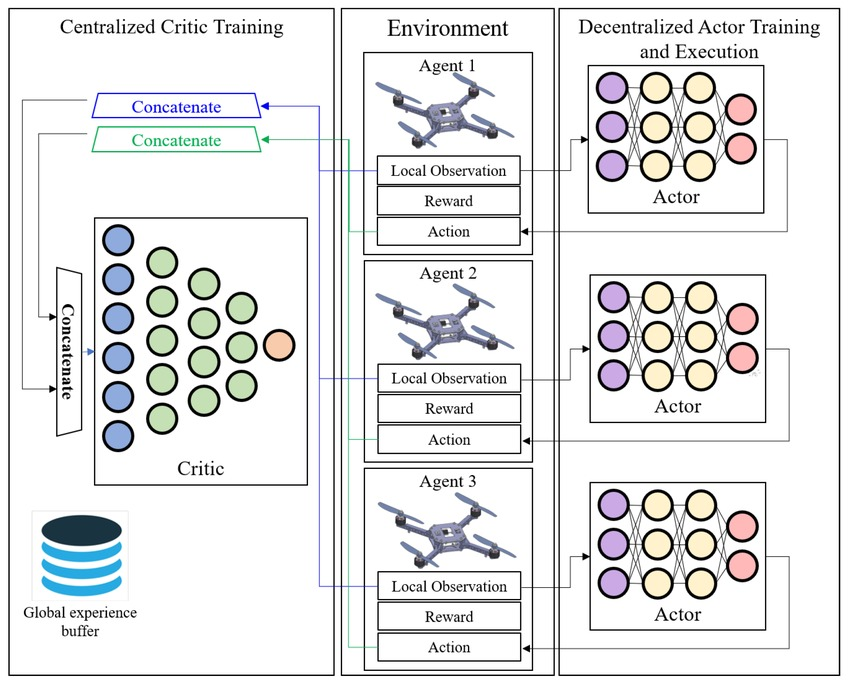
\includegraphics[width=0.4\textwidth]{img_pfe/ctde.jpeg}
    \caption{CTDE MARL framework for collaborative UAV swarm navigation.
   \parencite{swarm_navigation_ctde} }.
    \label{fig:ctde}
\end{figure}

Once training converges, the computationally expensive centralized critic is discarded. The final product is a set of efficient, decentralized actors capable of effective performance during execution, making the approach both powerful in training and practical in deployment.

\subsection{Key Assumptions of the CTDE Paradigm}
The popular CTDE paradigm, while powerful, relies on its own set of strong assumptions to function effectively.
\begin{itemize}
  \item Centralized Access During Training: The primary assumption is that a centralized controller can access global information (e.g., the full state or all agents' observations and actions) during a simulated training phase. This allows for efficient, coordinated learning, but may not be feasible in real-world scenarios where such a centralized simulator is unavailable.
    \item Factorizability of the Joint Value Function: Value-based CTDE methods, such as VDN and QMIX, assume that the team's joint action-value function ($Q_{\text{tot}}$) can be effectively represented as a combination of individual agent utilities ($Q_i$). This factorization is crucial for decentralized execution, but if the problem's true value function cannot be represented this way, these methods may fail to converge to the optimal policy.
\end{itemize}

\begin{figure}[H]
    \centering
   
        
    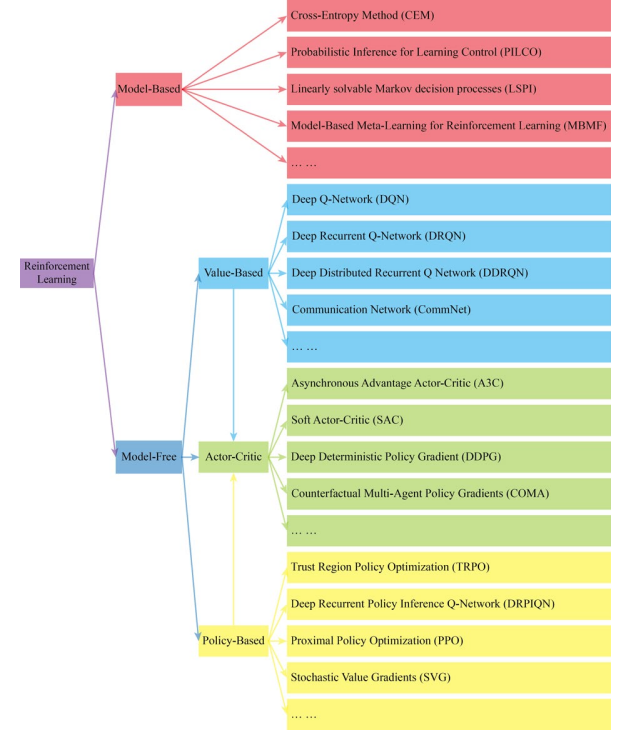
\includegraphics[width= 0.6\linewidth]{img_pfe/Classification_of_RL.PNG}
                \caption{Classification of reinforcement learning algorithms (Adapted from \parencite{smacv2_review})}
        \label{fig:classification_of_RL}
\end{figure}
    
\section*{Conclusion}

This chapter has charted a course from the well-defined world of single-agent reinforcement learning to the complex, dynamic frontier of multi-agent systems. We began with foundational principles, then journeyed into the multi-agent domain, where interacting learners give rise to profound challenges like non-stationarity and partial observability. In response, powerful frameworks like CTDE have emerged. However, we have also seen that CTDE is not a complete solution, as it introduces its own theoretical gaps related to scalability, representation, and factorization. It is precisely these gaps, especially the challenge of forming effective policies from limited, partial observations, that provide the motivation for our work in this report. Having established this theoretical landscape, we are now equipped to explore the state-of-the-art algorithms that attempt to navigate these complexities, before introducing our own proposed solution.
\chapter{State of the Art}
\label{chap:sota}  

\section*{Introduction}
This chapter provides a comprehensive review of the state-of-the-art in cooperative multi-agent reinforcement learning, with a specific focus on methods designed to address the challenge of partial observability. We begin by analyzing the foundational algorithms within the CTDE paradigm, such as Value-Decomposition Networks (VDN) and QMIX, which form the bedrock of modern cooperative MARL. We then transition to more advanced representation learning techniques that explicitly tackle the problem of missing information. This thematic analysis covers belief alignment methods like COLA, contrastive learning frameworks such as MA2CL, and, most critically, the reconstruction-based approach of the Multi-Agent Masked Auto-Encoder (${MA}^2E$), which serves as the direct foundation for our work. By critically evaluating the strengths and limitations of these approaches, this chapter establishes the research gap for a more adaptive and efficient masking strategy.

\section{Key Concepts and Terminology}

Before delving into the specific algorithms, this section defines several key concepts and recurring terminologies that are central to the state-of-the-art in cooperative MARL, particularly those addressing partial observability.

\paragraph{Value Decomposition}
A dominant strategy in value-based CTDE algorithms where the goal is to learn the global, joint action-value function ($Q_{tot}$) by factorizing it into individual utility functions ($Q_i$), one for each agent[cite: 2320, 736]. Foundational methods like VDN assume a simple summation, while more advanced methods like QMIX use a non-linear mixing network to combine the individual utilities.

\paragraph{The Monotonicity Constraint (IGM Principle)}
A crucial innovation introduced in QMIX that constrains its mixing network, ensuring that an increase in any individual agent's utility, $Q_i$, cannot cause a decrease in the total team value, $Q_{tot}$.This property is a sufficient condition to guarantee the Individual-Global-Max (IGM) principle, which ensures that a greedy action selection by each decentralized agent corresponds to the maximization of the global value function, making it critical for effective decentralized execution.

\paragraph{Centralized Critic}
A core component of policy-gradient-based CTDE methods like MADDPG and MAPPO.The critic is a value function that is used only during the training phase and is given access to global information, such as the full state and the actions of all agents. This allows it to provide a stable, low-variance learning signal (i.e., policy gradient) to guide the training of the decentralized actors (the agents' individual policies).

\paragraph{Advanced Representation Learning}
This refers to a class of techniques that aim to overcome the limitations of using a standard RNN to handle partial observability. Instead of just compressing an agent's history into a memory state, these methods focus on explicitly learning richer features or representations from partial observations. The goal is to allow agents to directly reason about or infer missing information about the true global state, either by aligning beliefs (like COLA) or by reconstructing the missing information (like ${MA}^2E$).

\paragraph{Masked Modeling}
A self-supervised learning paradigm where a model learns to reconstruct original data from a corrupted input, where parts have been "masked" or removed. This approach, popularized in NLP and computer vision, forces the model to learn a deep, contextual understanding of the data's underlying structure. In the context of MARL, this involves masking the trajectories of some agents and training a model to reconstruct them, thereby learning to infer global information from a partial view.
\section{Thematic Analysis}
% \lipsum[2]
% \subsection{Motivating Application: Coordination of  Unmanned Aerial Vehicles (UAVs) }
% A primary obstacle in applying reinforcement learning to robotics is the \textit{sim-to-real gap}: the significant discrepancy between the idealized physics and clean data of a simulator and the noisy, unpredictable dynamics of the physical world. A policy trained exclusively in a perfect simulation will likely fail upon deployment because it has not learned to handle real-world complexities like sensor noise, actuator lag, or environmental variations like wind. To address this critical challenge,\parencite{adversarial_domain_randomization} proposes a robust MARL framework designed to create policies that successfully transfer from simulation to real UAVs.

% Their approach is centered on a sophisticated technique known as \textbf{adversarial domain randomization (ADR)}. To understand ADR, it is useful to first consider standard domain randomization, where parameters of the simulation (e.g., mass, friction, lighting) are randomly varied during training. This exposes the agent to a range of conditions, preventing it from overfitting to a single, perfect simulation model. ADR enhances this process by introducing a second machine learning agent \textbf{an adversary} whose goal is to actively find the most difficult set of environmental parameters to make the primary agents fail. This creates an intelligent and adaptive training curriculum. Instead of randomly encountering challenging scenarios, the adversary systematically generates worst-case conditions, forcing the main agents to learn policies that are maximally robust.

% This adversarial training is complemented by an improved experience replay mechanism that prioritizes transitions with high temporal difference (TD) errors. This focuses the learning process on the most surprising or informative events, enhancing both training stability and sample efficiency.

% \paragraph{Strength} The key contribution of this work is a powerful method for bridging the sim-to-real gap, producing highly robust policies that generalize well from simulation to tangible, real-world UAV deployment.

% \paragraph{Limitations} However, the framework's focus is squarely on the sim-to-real problem for individual agent robustness. It does not fundamentally address the core MARL challenge of partial observability that arises from inter-agent interactions, nor is it designed to scale to large, complex swarms where decentralized coordination is the primary bottleneck.
%--------- old ---------------------------------------------------
% While some research focuses on the sim-to-real problem, \parencite{fuzzy_maddpg} tackles the challenge of coordination in uncertain, communication-limited environments, such as multi-UAV search and rescue. They propose a Fuzzy Deep Reinforcement Learning (Fuzzy-DRL) framework that enhances the popular MADDPG algorithm by integrating two key concepts: fuzzy logic and entropy-based rewards.

% Fuzzy logic is a powerful mathematical framework for reasoning with imprecise or incomplete information.
% %, moving beyond the traditional binary logic of ``true'' or ``false.'' Instead of requiring precise numerical inputs (e.g., ``distance is exactly 20.5 meters''), it allows for reasoning with linguistic variables that have degrees of truth (e.g., a UAV can be considered ``close,'' ``nearby,'' or ``far''). 
% In this context, fuzzy rules are used to intelligently manage the agents' reliance on communication. 
% % For example, a rule might state: ``IF an ally is 'very close' AND my task uncertainty is 'low', THEN my reliance on their communicated message is 'very low'.''
% This allows the system to gracefully handle intermittent or noisy communication without catastrophic failure.

% To improve the agents' ability to explore their environment, the authors incorporate entropy-based rewards. In reinforcement learning, entropy is a measure of the randomness or unpredictability of an agent's policy. By adding the entropy of its action distribution to the main task reward, the agent is intrinsically rewarded for trying new and diverse actions, preventing it from prematurely converging to a suboptimal strategy.

% \paragraph{Strength} The primary advantage of this hybrid method is its ability to create robust coordination strategies that can better handle the uncertainty inherent in real-world environments, particularly when communication is unreliable or limited.

% \paragraph{Limitation} The framework's main drawback lies in its scalability. Fuzzy logic systems rely on a set of human-engineered rules. As the number of agents and the complexity of their interactions increase, designing, managing, and tuning this rule set can become complex, making the approach less scalable than methods that learn all behaviors end-to-end.
%--------- old ---------------------------------------------------

% While some research focuses on the \textbf{sim-to-real} problem, \parencite{fuzzy_maddpg} tackles the challenge of coordination in uncertain, communication-limited environments typical of multi-UAV search and rescue. They propose a \textbf{Fuzzy Deep Reinforcement Learning (Fuzzy-DRL)} framework that enhances the popular \textbf{MADDPG} algorithm by integrating two key concepts: \textbf{fuzzy logic} and \textbf{entropy-based} rewards.

% The first component, fuzzy logic, is introduced to handle ambiguity and reason with imprecise data. Unlike classical logic, which operates on binary true/false values, fuzzy logic uses degrees of truth, allowing variables to belong partially to different sets. It operates on linguistic variables (e.g., distance can be described as \textit{close} or \textit{far}) which are mapped via membership functions to a value between 0 and 1. In this framework, fuzzy rules intelligently modulate the weight given to communicated information from teammates based on factors like distance or data uncertainty. This mechanism allows the system to gracefully degrade its reliance on communication when it is noisy or unavailable, preventing catastrophic failures and enhancing operational robustness.

% To improve the agents' learning process, the authors incorporate \textbf{entropy-based rewards}. In information theory, entropy quantifies the uncertainty or randomness in a distribution. Within reinforcement learning, adding an entropy bonus to the reward function drives the agent to maintain a more stochastic policy (one that does not collapse to a single, deterministic action for a given state ). This has two benefits: it drives better exploration during training by encouraging the agent to try diverse actions, and it results in a less predictable final policy, which can be more robust in complex, dynamic environments.

% The primary strength of this hybrid method is its ability to produce coordination strategies that are inherently more resilient to environmental uncertainty and unreliable communication. However, the framework's main drawback is its scalability. Fuzzy logic systems depend on a set of human-engineered rules and membership functions. As the number of agents and the complexity of their interactions grow, the design and tuning of this rule-based system can become combinatorially complex, making the approach difficult to scale compared to end-to-end learning methods.
% To more directly address the core challenge of partial observability in multi-agent systems,\parencite{collaborative_decision-making} introduces a MARL method for multi-UAV collaboration built on a sophisticated actor-critic architecture. Their framework's novelty lies in the explicit combination of two powerful neural network components: recurrent networks and attention mechanisms.

% First, to handle the temporal nature of partial observability, each agent's policy is equipped with a Recurrent Network (RNN), such as a Gated Recurrent Unit (GRU) or Long Short-Term Memory (LSTM). An RNN processes sequences of observations, maintaining an internal hidden state that acts as a memory. This allows the agent to build a \textit{belief} or context from its observation history, rather than reacting solely to its most recent perception, which is crucial in environments where the full state is not visible at once.

% Building on this memory-based approach, the authors integrate an attention mechanism. While an RNN provides a compressed history, not all past information is equally relevant to the current decision. The attention mechanism allows the model to dynamically weigh the importance of different parts of its input, be it different elements of its own observation history or information communicated by different teammates. By learning to focus on the most salient information, the agent can make more informed and contextually aware decisions.

% The primary strength of this combined architecture is its ability to significantly improve coordination in partially observable settings by equipping agents with both a robust memory (from RNNs) and a method for selective focus (from attention). However, this enhanced capability comes with a significant limitation: both recurrent and attention layers add considerable computational complexity. This results in a model that is more computationally expensive and parameter-heavy, leading to longer training times and reduced efficiency, which can hinder its application in large-scale systems.
% \subsection{Motivating Application: Coordination of Unmanned Aerial Vehicles (UAVs)}
\subsection{Coordination of Unmanned Aerial Vehicles (UAVs)}
Research in multi-agent UAV coordination has produced solutions for several distinct challenges. To bridge the critical \textit{sim-to-real gap}, where policies trained in simulators fail in the real world, \parencite{adversarial_domain_randomization} uses adversarial domain randomization. This technique employs an adversary to generate worst-case environmental conditions in the simulator, forcing the agents to learn highly robust policies. While powerful for sim-to-real transfer, this method does not fundamentally address the MARL challenge of partial observability.

% To handle coordination under communication uncertainty, \parencite{fuzzy_maddpg} enhance the \textbf{MADDPG} algorithm with a \textit{Fuzzy-DRL} framework. This method uses pre-defined fuzzy logic rules to intelligently manage unreliable communication and incorporates \textit{entropy-based rewards}  to encourage exploration. The resulting system is more resilient to communication loss, but its reliance on hand-crafted fuzzy rules creates a significant scalability bottleneck.

To handle coordination under communication uncertainty, \parencite{fuzzy_maddpg} enhances the \textbf{MADDPG} algorithm with a \textit{Fuzzy Deep Reinforcement Learning} (Fuzzy-DRL) framework. This approach integrates two key concepts: \textit{fuzzy logic} and \textit{entropy-based rewards}. The first component, fuzzy logic, is introduced to manage ambiguity by reasoning with linguistic variables (e.g., describing distance as \textit{close} or \textit{far}) rather than relying on precise numerical values. Within this framework, human-engineered fuzzy rules intelligently modulate the weight assigned to information communicated by teammates based on factors such as distance or data uncertainty. This enables the system to gracefully handle noisy or intermittent communication, thereby enhancing operational robustness. To further improve learning, the authors incorporate entropy-based rewards: by adding an entropy bonus to the reward function, the agent is implicitly encouraged to maintain a more stochastic policy, which improves exploration and results in a more robust and less predictable final policy. While the system is highly tolerant of communication loss, its reliance on a hand-crafted rule set introduces a significant scalability limitation as the number of agents and the complexity of their interactions increase.

More directly addressing partial observability,
\parencite{collaborative_decision-making} combine Recurrent Networks (RNNs) to provide agents with a memory of past observations, and attention mechanisms to allow them to focus on the most salient information within that memory. This combination of memory and selective focus improves coordination, but at the cost of significant computational complexity that hinders its use in large-scale systems.

Collectively, these approaches highlight that targeted solutions for specific UAV problems often introduce scalability challenges or do not solve the underlying representation problem of partial observability, motivating the need for more general and efficient methods discussed next.
\subsection{The CTDE Paradigm and its Core Implementations}
\label{subsec:ctde}
Research within the CTDE paradigm has produced several algorithmic families designed to balance effective learning with scalable execution. These methods learn centrally but act decentrally, and are broadly categorized into value-decomposition and policy-gradient approaches.

% \paragraph{Value-Decomposition Network (VDN)}
% The foundational value-decomposition method is the Value-Decomposition Network (VDN), introduced by \parencite{VDN}. Its core mechanic is to learn a decomposed representation of the team's joint action-value function, $Q_{\text{tot}}$, by assuming it can be represented as a simple sum of individual agents' utility functions, $Q_i$, each conditioned only on an agent's local observation-action history. The total team value is thus calculated according to Equation~\eqref{eq:vdn}:

% \begin{equation}
%     \label{eq:vdn}
%     Q_{\text{tot}}(\tau,u) = \sum_{i=1}^{n} Q_i(\tau_i, u_i)
% \end{equation}

% where:
% \begin{itemize}
%     \item $Q_{\text{tot}}(\tau, u)$ is the total action-value for the team, given the joint action-observation history $\tau$ and the joint action $u$.
%     \item $Q_i(\tau_i, u_i)$ is the individual utility function learned by agent $i$, based on its own local history $\tau_i$ and its individual action $u_i$.
%     \item $n$ is the total number of agents.
% \end{itemize}

% During training, VDN uses a shared replay buffer to calculate the TD-error based on this global $Q_{\text{tot}}$, and the resulting loss is backpropagated through the summation to implicitly update each individual $Q_i$ network without needing agent-specific rewards. The primary advantage of this structure is that it enables efficient, decentralized execution; since maximizing the sum of the utilities is equivalent to maximizing each one individually, each agent can simply act greedily with respect to its own local utility function during deployment. This makes the approach highly scalable and more effective than fully centralized or independent learning methods. However, VDN's fundamental drawback lies in its restrictive additive assumption. By forcing a linear decomposition, VDN cannot represent more complex, non-linear interactions between agents where one's contribution is conditional on the actions of others.
% \begin{figure}
%     \centering
%     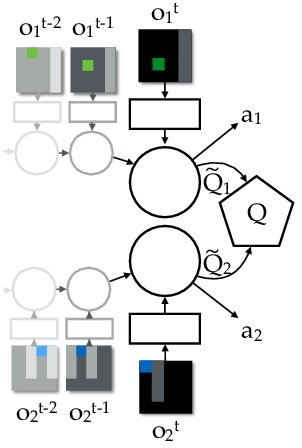
\includegraphics[width=0.5\linewidth]{img_pfe/vdn.png}
%     \caption{Enter Caption}
%     \label{fig:vdn}
% \end{figure}
The foundational value-decomposition method is the Value-Decomposition Network (VDN), introduced by \parencite{VDN}. Its core mechanic is to learn a decomposed representation of the team's joint action-value function, $Q_{\text{tot}}$, by assuming it can be represented as a simple sum of individual agents' utility functions, $Q_i$. The VDN architecture, illustrated for a two-agent case in Figure~\ref{fig:vdn_architecture}, shows how each agent's network processes its own local observation history ($\tau_i$) to produce an individual utility value ($\tilde{Q}_i$). These individual values are then combined by a simple summation to produce the total team value, $Q_{\text{tot}}$. The total team value is thus formally calculated as shown in Equation~\eqref{eq:vdn}:



\begin{equation}
    \label{eq:vdn}
    Q_{\text{tot}}(\tau,u) = \sum_{i=1}^{n} Q_i(\tau_i, u_i)
\end{equation}

Where:
\begin{itemize}
    \item $Q_{\text{tot}}(\tau, u)$ is the total action-value for the team, given the joint action-observation history $\tau$ and the joint action $u$.
    \item $Q_i(\tau_i, u_i)$ is the individual utility function learned by agent $i$, based on its own local history $\tau_i$ and its individual action $u_i$.
    \item $n$ is the total number of agents.
\end{itemize}

During training, VDN uses a shared replay buffer to calculate the TD-error based on this global $Q_{\text{tot}}$, and the resulting loss is backpropagated through the summation to implicitly update each individual $Q_i$ network without needing agent-specific rewards. The primary advantage of this structure is that it enables efficient, decentralized execution; since maximizing the sum of the utilities is equivalent to maximizing each one individually, each agent can simply act greedily with respect to its own local utility function during deployment. This makes the approach highly scalable and more effective than fully centralized or independent learning methods. However, VDN's fundamental drawback lies in its restrictive additive assumption. By forcing a linear decomposition, VDN cannot represent more complex, non-linear interactions between agents where one's contribution is conditional on the actions of others.
% \begin{figure}[H] 
%     \centering
%     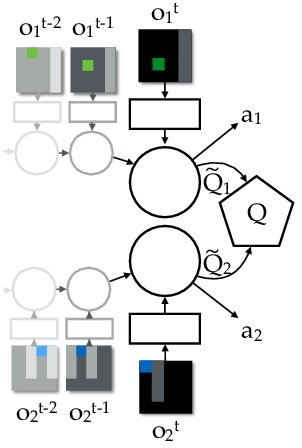
\includegraphics[width=0.3\textwidth]{img_pfe/vdn.png} 
%     \caption{The architecture of a Value-Decomposition Network (VDN) for two agents. Each agent's network processes local observations ($O_1, O_2$) through recurrent layers to produce individual utility values ($\tilde{Q}_1, \tilde{Q}_2$). These are then summed to form the joint Q-value ($Q$), which is used for centralized training. (Adapted from \parencite{VDN}).}
%     \label{fig:vdn_architecture}
% \end{figure}
% Use the standard 'figure' environment as a floating wrapper
% This is the code for your side-caption figure.
% It uses minipage and is fully compatible with the 'caption' package.

\begin{figure}[H]
    
    % --- Box for the image ---
    % I've set its width to 35% of the text width.
    \begin{minipage}{0.3\textwidth}
        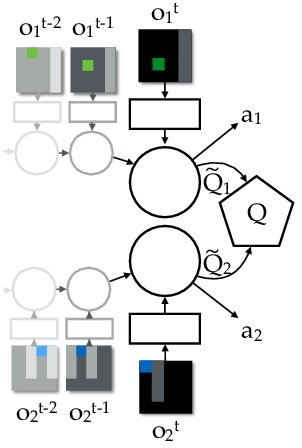
\includegraphics[width=\linewidth]{img_pfe/vdn.png}
    \end{minipage}
    \hspace{0.07\textwidth} 
    \begin{minipage}{0.5\textwidth}

        \captionof{figure}{The architecture of a Value-Decomposition Network (VDN) for two agents. Each agent's network processes local observations ($O_1, O_2$) through recurrent layers to produce individual utility values ($\tilde{Q}_1, \tilde{Q}_2$). These are then summed to form the joint Q-value ($Q$), which is used for centralized training. (Adapted from \parencite{VDN}).}
        \label{fig:vdn_architecture}
    \end{minipage}

\end{figure}
% \paragraph{QMIX}
% To address the expressive limitations of VDN, QMIX was introduced as a more sophisticated value-decomposition algorithm. QMIX replaces the simple summation with a non-linear mixing network that takes all individual agent utilities, $Q_i$, as input to produce the team value, $Q_{\text{tot}}$. The crucial innovation is that the weights of this mixing network are constrained to be non-negative, enforcing an overall monotonicity constraint on the relationship between individual and team values:
% $$
% \frac{\partial Q_{\text{tot}}}{\partial Q_i} \geq 0
% $$
% This elegant constraint guarantees the Individual-Global-Max (IGM) principle, which ensures that a greedy action selection by each decentralized agent still leads to the maximization of the global team value. This allows QMIX to represent a much richer class of functions than VDN, capturing more complex agent synergies while still permitting tractable decentralized execution. Despite its advantages, the monotonicity requirement still imposes a structural constraint on the types of value functions that can be learned, which may not be sufficient for all possible multi-agent coordination problems.
% To address the expressive limitations of VDN, QMIX, introduced by \parencite{QMIX}, provides a more sophisticated value-decomposition approach. QMIX replaces the simple summation with a non-linear mixing network that takes all individual agent utilities, $Q_i$, as input to produce the team value, $Q_{\text{tot}}$. The overall architecture, depicted in Figure~\ref{fig:qmix_architecture}, consists of individual agent networks (c) that produce utility values, which are then fed into a central mixing network (b). The crucial innovation of QMIX lies in this mixing network (a), which enforces a monotonicity constraint on the relationship between individual and team values:
% \begin{equation*}
%     \frac{\partial Q_{\text{tot}}}{\partial Q_i} \geq 0
% \end{equation*}
% This is achieved by using hypernetworks (in red) that take the global state $s_t$ as input and generate the weights for the mixing network, ensuring they are non-negative. The entire end-to-end system is then trained to minimize a standard temporal-difference loss over the joint action-value function, as shown in Equation~\eqref{eq:qmix_loss}:



% \begin{equation}
%     \label{eq:qmix_loss}
%     L(\theta) = \sum_{i=1}^{b} \left[ \left(y^{i}_{\text{tot}} - Q_{\text{tot}}(\tau, u, s; \theta)\right)^2 \right]
% \end{equation}

% where:
% \begin{itemize}
%     \item $L(\theta)$ is the loss function parameterized by the network weights $\theta$.
%     \item $b$ is the batch size of transitions sampled from the replay buffer.
%     \item $Q_{\text{tot}}(\tau, u, s; \theta)$ is the joint action-value function produced by the mixing network.
%     \item $y_{\text{tot}}$ is the target value (TD target), calculated as: 
%     \begin{equation*}
%          y_{\text{tot}} = r + \gamma \max_{u'} Q_{\text{tot}}(\tau', u', s'; \theta^{-})
%     \end{equation*}
   
%     where $\theta^{-}$ represents the parameters of a periodically updated target network.
% \end{itemize}

To address the expressive limitations of VDN, QMIX, introduced by  \parencite{QMIX}, provides a more sophisticated value-decomposition approach. It replaces the simple summation with a non-linear mixing network that takes all individual agent utilities, $Q_i$, as input to produce the team value, $Q_{\text{tot}}$. The overall architecture, depicted in Figure~\ref{fig:qmix_architecture}, shows how individual agent networks feed their utilities into this central mixing network. The crucial innovation of QMIX lies in enforcing a monotonicity constraint on this network, ensuring that an increase in any individual utility does not cause a decrease in the team value:
\begin{equation*}
    \frac{\partial Q_{\text{tot}}}{\partial Q_i} \geq 0
\end{equation*}
This is achieved by using hypernetworks that take the global state $s_t$ as input and generate non-negative weights for the mixing network, allowing the system to leverage centralized information during training.

The entire end-to-end system is trained by minimizing a temporal-difference (TD) loss function over batches of experience sampled from a replay buffer. This loss is defined as:
\begin{equation}
    \label{eq:qmix_loss}
    L(\theta) = \sum_{i=1}^{b} \left[ \left(y_{\text{tot}} - Q_{\text{tot}}(\tau, u, s; \theta)\right)^2 \right]
\end{equation}
Here, the target value $y_{\text{tot}}$ is calculated using the standard Bellman update,\begin{equation*}
    y_{\text{tot}} = r + \gamma \max_{u'} Q_{\text{tot}}(\tau', u', s'; \theta^{-})
\end{equation*}
, where $r$ is the team reward, $\gamma$ is the discount factor, and $\theta^{-}$ are the parameters of a separate, periodically updated target network.

The primary advantage of this monotonic design is that it is a sufficient condition to guarantee the \textbf{Individual-Global-Max (IGM) } principle. The IGM principle ensures that a greedy action selection by each decentralized agent still corresponds to the maximization of the global team value, which is critical for effective decentralized execution. This allows QMIX to represent a much richer class of non-linear functions than VDN while maintaining tractability. However, despite its advantages, the monotonicity constraint also forms the primary limitation of QMIX, as it cannot represent non-monotonic value functions that can arise in problems where an agent's best action depends on the simultaneous actions of its teammates.
\begin{figure}[H]
    % \centering
    \begin{minipage}{0.6\textwidth}
        
    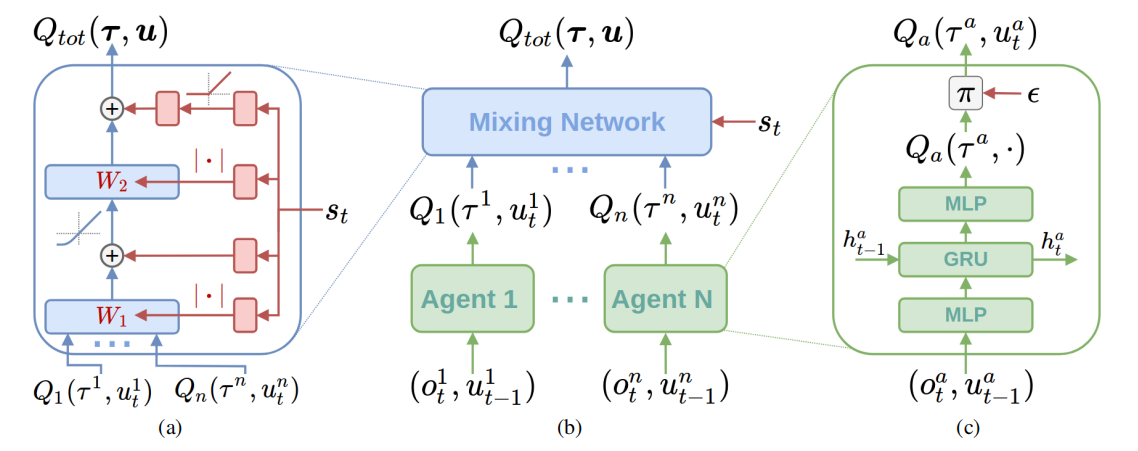
\includegraphics[width=\linewidth]{img_pfe/QMIX.PNG}
    \end{minipage}
    \hspace{0.05\textwidth} 
    \begin{minipage}{0.3\textwidth}
       
                \captionof{figure}{The QMIX architecture. (a) The mixing network ;(b) The central mixing network; (c) Agent network (Adapted from \parencite{QMIX})}
        \label{fig:qmix_architecture}
    \end{minipage}
\end{figure}
The primary advantage of this design is that the monotonicity is a sufficient condition to guarantee the \textbf{Individual-Global-Max (IGM)} principle, which ensures that a greedy action selection by each decentralized agent still corresponds to the maximization of the global team value. This allows QMIX to represent a much richer class of non-linear functions than VDN while still permitting tractable decentralized execution. However, despite its advantages, the monotonicity constraint also forms the primary limitation of QMIX, as it cannot represent non-monotonic value functions that can arise in problems where an agent's best action depends on the simultaneous actions of its teammates.

For environments with continuous action spaces, policy-gradient methods are the standard, with Multi-Agent Deep Deterministic Policy Gradient (MADDPG) being the canonical algorithm. Developed by  \parencite{MADDPG}, MADDPG adapts the single-agent DDPG actor-critic framework to the multi-agent domain by leveraging the CTDE paradigm in a unique way. While each agent's actor (policy) is decentralized and selects actions based only on its own local observations, the critic is centralized during training. Specifically, the critic is augmented with the observations and actions of all other agents. This centralized action-value function, $Q_i^{\mu}(x, a_1, \dots, a_N)$, allows the critic to form a stable learning signal, as the environment is stationary from its perspective even when other agents' policies are changing. The decentralized actor is then updated using the gradient provided by this centralized critic. The primary advantage of this structure is its flexibility and stability; it effectively solves the non-stationarity problem that challenges other methods and can be applied to cooperative, competitive, or mixed-motive settings, as each agent can learn its own unique critic and reward function. However, MADDPG's main limitation is that the input to the centralized critic grows linearly with the number of agents, which can be impractical for very large systems. Furthermore, the critic's update requires knowledge of other agents' actions during training, an assumption that, while common in simulations, can be restrictive.
% \paragraph{Multi-Agent Deep Deterministic Policy Gradient (MADDPG)}
% For environments with continuous or high-dimensional action spaces, the standard approach is the policy-gradient algorithm, Multi-Agent Deep Deterministic Policy Gradient (MADDPG). This method extends the single-agent DDPG framework by employing a specialized actor-critic architecture within the CTDE paradigm. While each agent's actor (policy) is decentralized and acts based only on its local observations, its corresponding critic is centralized during training. The critic is augmented with the observations and actions of all other agents, which provides it with a complete picture of the joint action and stabilizes the learning environment by resolving the non-stationarity problem. This allows for a robust training signal to be delivered to the decentralized actors. The flexibility of MADDPG makes it highly effective for complex control tasks, and it is often enhanced with recurrent networks and attention to better handle partial observability. Its primary limitation, however, is that policy-gradient methods are generally less sample-efficient and more computationally demanding than their value-based counterparts.
% Building upon the CTDE paradigm, this section details the influential algorithms that have defined modern cooperative MARL. These methods leverage a centralized training perspective to learn robust, coordinated policies that can be executed in a fully decentralized manner. We review the two primary algorithmic families that realize this paradigm: value-decomposition and policy-gradient methods.

% \subsubsection{Value-Decomposition Methods: Scalable Coordination}
% Value-decomposition methods are highly effective and scalable, particularly in tasks with discrete action spaces. They learn a factorized team value function ($Q_{\text{tot}}$) based on individual agent utilities ($Q_i$).

% \paragraph{VDN} As the foundational method, VDN proposes the simplest factorization, representing $Q_{\text{tot}}$ as a direct sum of individual agent values:
% $$
% Q_{\text{tot}}(\tau,u) = \sum_{i=1}^{n} Q_i(\tau_i, u_i)
% $$
% \textbf{Strength:} The primary advantage of VDN is its simplicity and scalability. \textbf{Limitation:} Its core assumption of linear additivity is a significant restriction, as it cannot represent more complex, non-linear synergies between agents.

% \paragraph{QMIX} This highly influential algorithm overcomes VDN's limitations by using a non-linear mixing network. This network takes the individual $Q_i$ values as input and combines them to estimate $Q_{\text{tot}}$. The crucial innovation in QMIX is that the mixing network's weights are constrained to be non-negative, which enforces an overall monotonicity constraint:
% $$
% \frac{\partial Q_{\text{tot}}}{\partial Q_i} \geq 0
% $$
% \textbf{Strength:} This constraint cleverly guarantees the Individual-Global-Max (IGM) principle, ensuring that a decentralized greedy selection of actions by each agent still corresponds to the optimal joint action for the team. This makes it highly effective for decentralized execution. \textbf{Limitation:} While more expressive than VDN, the monotonicity requirement still restricts the class of functions it can represent and may not capture all complex agent dependencies.

% \subsubsection{Policy-Gradient Methods: Handling Complex Actions}
% For environments with continuous or high-dimensional action spaces, policy-gradient methods are the standard. The canonical algorithm in this domain is the Multi-Agent Deep Deterministic Policy Gradient (MADDPG).

% \paragraph{MADDPG} This algorithm adapts the popular single-agent DDPG framework to the multi-agent setting using a specialized actor-critic architecture. While each agent's actor (policy) remains decentralized, acting based only on local observations, the critic is centralized during training. Specifically, each agent's critic is augmented with the observations and actions of all other agents. This global perspective allows the critic to form a stable learning target, effectively solving the non-stationarity problem.

% \paragraph{Enhancements (e.g., Zhang et al.)} The base MADDPG architecture is often enhanced to better handle partial observability. This includes integrating recurrent policies to process observation histories and adding attention mechanisms to help agents focus on the most salient information.

% \textbf{Strength:} MADDPG and its variants excel in complex, continuous action spaces and can learn sophisticated policies. \textbf{Limitation:} This flexibility comes at a cost, as these methods are generally less sample-efficient and require more computational resources and training time than their value-based counterparts.
% --------------- MAPPO----------------------------
% In the domain of policy-gradient methods, \textbf{Multi-Agent Proximal Policy Optimization (MAPPO)} \parencite{ppo_ctde} has emerged as a surprisingly effective on-policy algorithm within the CTDE paradigm. 


% MAPPO's architecture consists of a decentralized actor and a centralized critic. Each agent's actor, or policy $\pi_{\theta}(a_i|o_i)$, is decentralized, mapping its own local observation $o_i$ to an action $a_i$. The critic, or value function $V_{\phi}(s)$, is centralized and utilized only during the training phase. This centralization allows the critic to access global state information $s$ that is unavailable to the agents during execution, providing a stable learning signal that helps mitigate the non-stationarity of the multi-agent environment. For environments with homogeneous agents, the parameters for both the actor and critic networks are typically shared across all agents to improve learning efficiency.
% The policy parameters $\theta$ are optimized by maximizing the PPO clipped surrogate objective, which includes an entropy bonus term to encourage exploration. The objective function is defined as:
% \begin{equation}
% \label{eq:actor_loss}
% \mathcal{L}(\theta) = \frac{1}{Bn} \sum_{i=1}^{n} \sum_{k=1}^{B} \left[ \min\left(r_{\theta,i}^{(k)} \hat{A}_i^{(k)}, clip(r_{\theta,i}^{(k)}, 1-\epsilon, 1+\epsilon) \hat{A}_i^{(k)}\right) \right] + \frac{\sigma}{Bn} \sum_{i=1}^{n} \sum_{k=1}^{B} S[\pi_{\theta}(o_i^{(k)})]
% \end{equation}
% where:
% \begin{itemize}
%     \item $r_{\theta, i}^{(k)} = \frac{\pi_{\theta}(a_i^{(k)} | o_i^{(k)})}{\pi_{\theta_{\text{old}}}(a_i^{(k)} | o_i^{(k)})}$ is the importance sampling ratio between the current and old policies.
%     \item $\hat{A}_i^{(k)}$ is the advantage estimate calculated using Generalized Advantage Estimation (GAE).
%     \item $\epsilon$ is a hyperparameter that defines the clipping range.
%     \item $S$ is the policy entropy and $\sigma$ is its coefficient hyperparameter.
% \end{itemize}

% \noindent Concurrently, the critic's parameters $\phi$ are trained to minimize a clipped mean-squared error loss between the predicted value $V_{\phi}(s_i^{(k)})$ and the calculated reward-to-go $\hat{R}_i$. The loss is given by:
% \begin{equation}
% \label{eq:critic_loss}
% \mathcal{L}(\phi) = \frac{1}{Bn} \sum_{i=1}^{n} \sum_{k=1}^{B} \max\left[ (V_{\phi}(s_i^{(k)}) - \hat{R}_i)^2, (clip(V_{\phi}(s_i^{(k)}), V_{\phi_{\text{old}}}(s_i^{(k)}) - \epsilon, V_{\phi_{\text{old}}}(s_i^{(k)}) + \epsilon) - \hat{R}_i)^2 \right]
% \end{equation}

% The primary advantage of MAPPO is its surprising effectiveness and strong empirical performance across a variety of cooperative MARL benchmarks. The research shows that with careful tuning of key implementation factors—such as value normalization, limited training epochs, minimal mini-batching, and a small clipping ratio—MAPPO can achieve results and sample efficiency that are competitive with, or even superior to, state-of-the-art off-policy methods. Its relative simplicity and effectiveness make it an exceptionally strong baseline for cooperative MARL research. However, the analysis presented is primarily empirical, with the algorithm's performance evaluated in cooperative, discrete action spaces with mostly homogeneous agents. Its applicability to more diverse settings, such as competitive games or environments with continuous action spaces, remains a direction for future work.

As an on-policy alternative in the policy-gradient family of algorithms, \textbf{Multi-Agent Proximal Policy Optimization (MAPPO)} \parencite{ppo_ctde} offers a robust framework for cooperative multi-agent tasks. It adapts the single-agent PPO algorithm to a multi-agent actor-critic setting, leveraging the CTDE paradigm to achieve surprisingly strong performance with minimal architectural complexity.


The core of MAPPO's architecture lies in its use of decentralized actors and a centralized critic. Each agent's actor, or policy $\pi_{\theta}(a_i | o_i)$, is decentralized and maps its local observation $o_i$ to an action $a_i$. To stabilize training in the non-stationary multi-agent environment, a centralized critic, or value function $V_{\phi}(s)$, is used during the training phase. This critic has access to global state information $s$, providing a consistent and stable learning signal for all actors.


The policy parameters $\theta$ are trained by maximizing the PPO clipped surrogate objective function, which constrains the magnitude of policy updates. This objective, which also includes an entropy bonus $S$ to encourage exploration, is defined as:
\begin{equation}
\label{eq:actor_loss}
\mathcal{L}(\theta) = \frac{1}{Bn} \sum_{i=1}^{n} \sum_{k=1}^{B} \left[ \min\left(r_{\theta,i}^{(k)} \hat{A}_i^{(k)}, clip(r_{\theta,i}^{(k)}, 1-\epsilon, 1+\epsilon) \hat{A}_i^{(k)}\right) \right] + \frac{\sigma}{Bn} \sum_{i=1}^{n} \sum_{k=1}^{B} S[\pi_{\theta}(o_i^{(k)})]
\end{equation}
Where $r_{\theta,i}^{(k)}$ is the importance sampling ratio, and $\hat{A}_i^{(k)}$ is the advantage estimate calculated using Generalized Advantage Estimation (GAE).

The centralized critic's parameters $\phi$ are trained to minimize a clipped mean-squared error loss between the predicted value $V_{\phi}(s_i^{(k)})$ and the calculated reward-to-go target $\hat{R}_i$:
\begin{equation}
\label{eq:critic_loss}
\mathcal{L}(\phi) = \frac{1}{Bn} \sum_{i=1}^{n} \sum_{k=1}^{B} \max\left[ (V_{\phi}(s_i^{(k)}) - \hat{R}_i)^2, \left(clip(V_{\phi}(s_i^{(k)}), V_{\phi_{\text{old}}}(s_i^{(k)}) - \epsilon, V_{\phi_{\text{old}}}(s_i^{(k)}) + \epsilon) - \hat{R}_i\right)^2 \right]
\end{equation}
The entire system is trained on-policy, meaning that for each update, a new batch of experience is collected using the current policy. The actor and critic networks are then updated for several epochs on this data using their respective objective functions.


The primary advantage of MAPPO is its surprising effectiveness and strong empirical performance across a variety of cooperative MARL benchmarks. The research demonstrates that with specific implementation practices such as value normalization and limited training epochs, MAPPO can achieve results and sample efficiency competitive with, or even superior to, state-of-the-art off-policy methods. Its relative simplicity and generality make it an exceptionally strong baseline for cooperative MARL research. Furthermore, its performance was evaluated mainly in cooperative, discrete action spaces, with its applicability to more diverse settings remaining an open question.

\subsection{Advanced Representation Learning for Partial Observability}
While foundational algorithms like QMIX and MADDPG are powerful, they share a common approach to partial observability: each agent's observation history is typically processed by a recurrent neural network (RNN) to produce a memory or belief state. This method, however, creates a significant information bottleneck, as it compresses an arbitrarily long history into a fixed-size vector, potentially losing crucial past information. Furthermore, this implicit memory state does not allow an agent to explicitly reason about what information is missing from its view or its importance. This core limitation has motivated a shift in the research community toward more sophisticated representation learning techniques that aim to directly address the missing information, either by learning to align agent beliefs about the hidden state or by learning to reconstruct it from a partial view. In this section, we review these two approaches.


% The first advanced approach, belief alignment, is exemplified by Consensus Learning for Cooperative Multi-Agent Reinforcement Learning (COLA), introduced by \parencite{COLA}. The work is inspired by concepts from computer vision, specifically \textit{viewpoint invariance and data augmentation}, where the local observations of different agents are treated as augmented views of the same underlying global state. COLA seeks to have agents learn a shared \textbf{consensus} from these different views.

% To achieve this, COLA employs a sophisticated contrastive learning framework. While traditional contrastive learning often relies on an \textbf{InfoNCE loss} with negative sampling, COLA adopts a more recent technique inspired by \textbf{Knowledge Distillation with No Labels (DINO)}. It uses a \textbf{consensus builder} module with a student-teacher network architecture. Both networks learn to map an agent's local observation to a probability distribution over $K$ discrete classes, where $K$ is a hyperparameter representing the number of possible consensus states. The system is trained by minimizing the cross-entropy loss between the student's output for one agent's view and the teacher's output for another agent's view:
Introduced by ~\parencite{COLA}, \textbf{Consensus Learning for Cooperative Multi-Agent Reinforcement Learning (COLA)} exemplifies a belief alignment approach inspired by concepts from computer vision, specifically \textit{viewpoint invariance} and \textit{data augmentation}. The core idea is to treat the different local observations of each agent as distinct ``views'' of the same underlying global state, from which the agents learn to infer a shared consensus without communication. To achieve this, COLA employs a \textbf{consensus builder} module based on a sophisticated contrastive learning framework. Unlike traditional methods that can rely on negative sampling, COLA is inspired by \textbf{Knowledge Distillation with No Labels (DINO)}, which uses a student-teacher network architecture. This module learns to map an agent's observation to a probability distribution over $K$ discrete consensus classes. The system is trained by minimizing the cross-entropy loss between the student network's output for one agent's view and the teacher's output for another's, encouraging different views of the same state to map to the same consensus label.
% \begin{equation*}
%     L_{\text{CB}} = \sum_{a,b} H\left(P_T(z_a), P_S(z_b)\right)
% \end{equation*}

% This process trains the consensus builder to map different local observation views to the same discrete consensus label (one of the $K$ classes).
This inferred one-hot consensus is then fed as an additional input into each agent's network, providing a shared cooperative signal during decentralized execution without any communication overhead. A key strength of COLA is that it can be integrated into various CTDE algorithms like QMIX or MADDPG to improve performance with only minor changes to the model architecture. However, its effectiveness is sensitive to the hyperparameter $K$.The optimal number of consensus classes must be tuned to the task's complexity, and the approach is less beneficial in scenarios where global consensus is not required.
\begin{figure}[H]
    \centering
         
    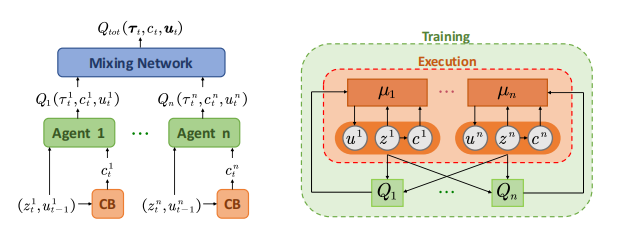
\includegraphics[width=0.6\linewidth]{img_pfe/marl_with_consensus learning.PNG}       
                \caption{Illustration of multi-agent reinforcement learning methods with consensus learning.\texttt{[Left]:} The value decomposition method with consensus learning. \texttt{[Right]:} The multi-agent actor-critic method with consensus learning (Adapted from \parencite{COLA})}
        \label{fig:marl_with_consensus_learning}
\end{figure}

% A key limitation of prior MARL representation learning methods is their primary focus on temporal awareness without explicitly learning from the rich correlational information between agents. To address this, \parencite{ma2cl} introduces the \textbf{Multi-Agent Masked Attentive Contrastive Learning (MA2CL)} framework, designed to learn representations that are simultaneously predictive in both the temporal and agent dimensions. The architecture of MA2CL, shown in Figure~\ref{fig:ma2cl_architecture}, operates as a self-supervised auxiliary task alongside a main MARL algorithm.

% The process, illustrated in Figure~\ref{fig:ma2cl_architecture}
% The process begins by "masking" a randomly selected agent by replacing its current observation and action ($o_t^i, a_t^i$) with data from the previous timestep ($o_{t-1}^i, a_{t-1}^i$). This masked sequence of observations, $\tilde{o}_t$, is passed through an Online Encoder ($\psi$) and an Online Projector ($\phi$) to produce a sequence of latent features, $\hat{z}_t$. The core of the framework is an Attentive Reconstruction model that takes this latent sequence, along with the masked actions $\tilde{a}_t$ and positional embeddings, to predict the latent representation of the masked agent, $\hat{y}_M$.




%------ MA2CL -----------------------
A key limitation of prior MARL representation learning methods is their primary focus on temporal awareness without explicitly learning from the rich correlational information between agents. To address this, \parencite{ma2cl} introduces the Multi-Agent Masked Attentive Contrastive Learning (MA2CL) framework, designed to learn representations that are simultaneously predictive in both the temporal and agent dimensions. The architecture of MA2CL, shown in Figure~\ref{fig:ma2cl_architecture}, operates as a self-supervised auxiliary task.


\begin{figure}[H] 
    \centering
    % Box for the image
        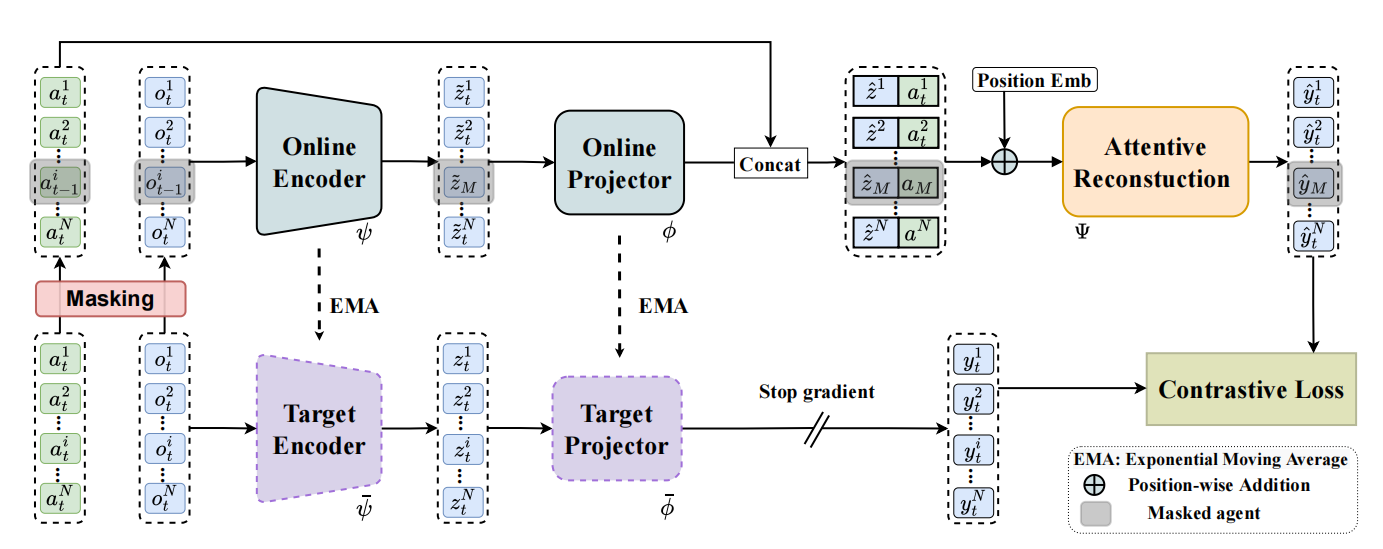
\includegraphics[width=\linewidth]{MA2CL.PNG}
   
    
        \caption{The framework of MA2CL. An online encoder and projector process masked observations, while a target network processes the original observations. An attentive reconstruction model predicts the latent features of the masked agents, which are then optimized via a contrastive loss against the target features. (Adapted from \parencite{ma2cl}).}
        \label{fig:ma2cl_architecture}
\end{figure}


It begins with a unique masking strategy in which a randomly selected agent’s current observation and action \((o^t_i, a^t_i)\) are replaced by its data from the previous timestep \((o^{t-1}_i, a^{t-1}_i)\). This masked input is then processed by a dual-stream architecture: a common design in contrastive learning, to prevent model collapse and promote stable training. An online encoder \(\psi\) and a non-linear projector \(\phi\) generate latent features from the masked data, while a target encoder \(\bar{\psi}\) and projector \(\bar{\phi}\) create stable features from the unmasked data. The target networks are updated using an exponential moving average (EMA) of the online network parameters, ensuring that target representations evolve smoothly and provide a consistent learning objective. 
An attentive reconstruction module then uses the online output to predict the masked agent’s true latent feature. The entire online network is optimized via an \textbf{InfoNCE contrastive loss} :
\begin{equation}
    \label{eq:ma2cl_loss}
    L_{\text{cl}} = \sum_{i=1}^{N} -M_i \log \left( \frac{\exp(\omega(q_i, k_i))}{\sum_{j=1}^{N} \exp(\omega(q_i, k_j))} \right)
\end{equation}

Here, the query $q_i$ is the reconstructed feature $\hat{y}_i$, the positive key $k_i$ is the true feature $y_i$ for the same agent, and the negative keys are the features $y_j$ of all other agents. This loss pushes the model to reconstruct an agent's representation accurately while distinguishing it from its teammates. 

%, which frames the prediction as a classification task: it aims to match each agent’s reconstructed latent representation to its true target representation $y_t$ among a set of distractors derived from the other agents’ features.
A \textit{stop-gradient} operation is applied to the target network outputs during loss computation to avoid a degenerate solution where both networks collapse to trivial representations. By minimizing this loss, MA2CL compels the encoder to produce rich and informative features, thereby enhancing both the quality of representation learning and the overall sample efficiency of the MARL policy.


The strength of this approach is that it forces the encoder to learn both temporal and agent-level context, significantly improving the sample efficiency and performance of the base MARL algorithm. However, a potential limitation is that such a specialized auxiliary task may encourage the representations to be highly optimized for final performance on a specific benchmark, potentially at the cost of broader generalization to different tasks.

%-------MaskMA----------------------------------
Recent work in MARL has increasingly adopted Transformer-based models to treat multi-agent decision-making as a sequence modeling problem, with notable examples including MADT\parencite{MADT}  Appendix~\ref{sec:MADT}   and MAT\parencite{MAT}  Appendix~\ref{sec:MAT}. However, these powerful architectures face two critical challenges. The first is a mismatch between their centralized training and decentralized execution; a Transformer trained on the full state of all agents struggles when executed with only partial, local observations. The second is poor generalization across tasks with varying numbers of agents and action spaces, as the meaning of the action vector can change completely from one task to another.

To address these limitations, \parencite{maskma} introduces the Mask-Based Collaborative Learning for \textbf{Multi-Agent Decision Making (MaskMA) } framework. To solve the training-execution mismatch, MaskMA employs a Mask-based Training Strategy (MTS), Figure~\ref{fig:MTS_MaskMa}. Instead of masking input tokens, it randomly masks connections within the Transformer's attention matrix during training, which forces the model to learn from partial information and thus better aligns the training phase with decentralized deployment. To handle the generalization problem, it uses a Generalizable Action Representation (GAR) that categorizes actions as either intrinsic (self-related) or interactive (other-related). By computing interactive actions based on the features of both the acting and target agents, the action representation becomes independent of the total number of agents, allowing for seamless transfer.
\begin{figure}[H]
    \begin{minipage}{0.5\textwidth}
       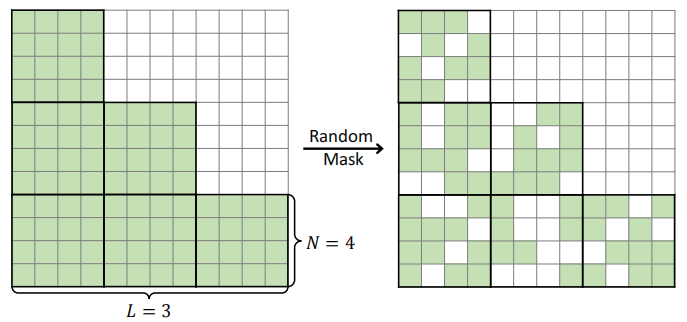
\includegraphics[width=\linewidth]{img_pfe/attention_matrix_MTS_MaskMa.PNG}
    \end{minipage}
    \hspace{0.07\textwidth} 
    \begin{minipage}{0.4\textwidth}

        \captionof{figure}{Visualization of the attention matrix in MTS. Left: The attention matrix displays a causal structure along the timestep
dimension, complemented by a non-causal configuration within each discrete timestep. Right: The final attention matrix used for training is obtained by randomly masking elements of the left attention matrix. (Adapted from \parencite{maskma}).}
        \label{fig:MTS_MaskMa}
    \end{minipage}

\end{figure}
The primary strength of this design is MaskMA's powerful zero-shot capability; the authors show that a single model trained on only 11 maps can achieve a 77.8\% win rate on 60 unseen test maps and can adapt to dynamic downstream tasks like ad hoc team play and ally malfunction. However, the framework's main limitation is its reliance on pre-collected, high-quality expert datasets for its imitation learning approach, and its generalization to entirely new game environments beyond its training domain is an area for future work.

% While prior self-supervised methods like MA2CL and MaskMA introduced masking to MARL, they often neglect the natural structure of partial observability, where an agent's local view is inherently a masked version of the global state. To address this, \parencite{ma2rl} proposes Masked Autoencoders for Multi-Agent Reinforcement Learning (MA2RL), a framework that improves agent collaboration by explicitly modeling and reconstructing the relationship between observed and unobserved entities. The MA2RL process first uses a Variational Autoencoder (VAE) to encode all observable entities into a latent space. Then, a recurrent network (GRU) uses this latent information and historical context to infer the representations of all unobserved (masked) entities. This reconstructed global view of all entities is then used to select a task-independent skill. Finally, an attentive action decoder generates an action based on both the skill and the complete (observed + inferred) entity information. A key aspect of this approach is the joint training of the reconstruction module and the policy itself, allowing the representation learning to be directly guided by the policy's needs. \textbf{The primary strength of MA2RL} is that by explicitly reasoning about and reconstructing the unobserved world from an entity perspective, it learns more generalizable and useful representations for coordination, leading to strong zero-shot performance. \textbf{However, this complex architecture}, which involves joint optimization of multiple components including VAEs and a policy network, may require more training steps and careful handling of multiple supervision signals to converge effectively.

%-----------MA2RL---------

While prior skill-based methods struggle to achieve team awareness under partial observability, and other masking techniques like MA2CL use \textit{artificial} masking strategies, a more direct approach is needed to handle an agent's limited view. These earlier methods do not treat an agent's line of sight as a natural mask of the full environment from an entity-centric perspective. To address this specific problem, \parencite{ma2rl} proposes Masked Autoencoders for Multi-Agent Reinforcement Learning (MA2RL). The core idea of MA2RL is to treat partial observability as a natural masking problem from an \textbf{entity perspective}. It views the environment as a collection of entities (allies, enemies, etc.), where an agent's local observation is simply a partial list of these entities, and all others are considered \textbf{masked} by being out of sight.

The MA2RL framework Figure~\ref{fig:ma2rl_architecture} and Figure~\ref{fig:ma2rl_att_decoder}  is designed to reconstruct a complete picture of the environment by inferring the states of these unobserved entities. It first uses a Variational Autoencoder (VAE)\parencite{vae} to encode the visible entities into a latent space. Then, a recurrent network (GRU) uses this information and past history to infer the latent representations of all the currently unobserved (masked) entities. This reconstructed global view, containing both observed and inferred entities, is then used to learn more generalizable, task-independent skills. The primary strength of this approach is its ability to learn a rich and complete representation of the world, leading to improved coordination and remarkable zero-shot generalization capabilities. However, the framework's complex, multi-component architecture, which jointly optimizes VAEs, a recurrent network, and the policy, may require significant training steps and careful management of its various supervision signals.

\begin{figure}[H] 
    \centering
    % Box for the image
        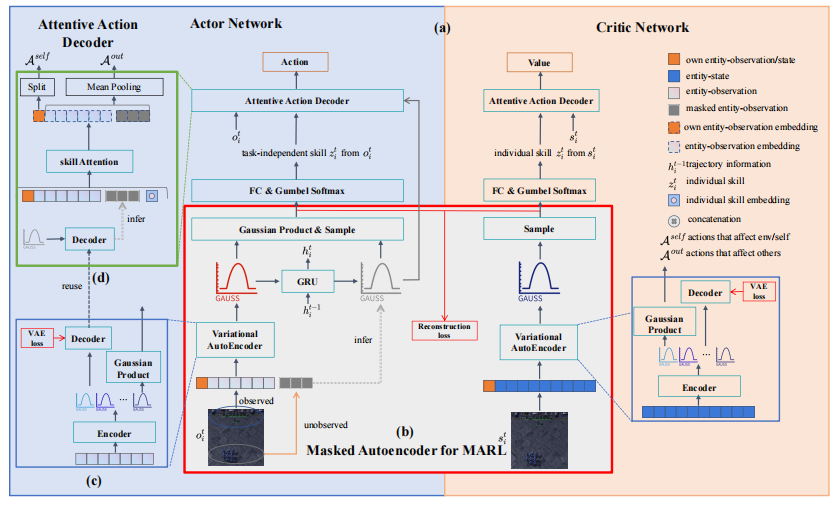
\includegraphics[width=\linewidth]{img_pfe/MA2RL.PNG}
   
    
        \caption{The network structure of MA2RL. (a) The overall architecture. (b) The structure of VAE. (c) The details of the masked autoencoder for MARL, where entity-observations can be regarded as a mask of the entity-states. (d) The attentive Action decoder that reuses the decoder in
VAE to infer masked entity-observations for better action execution. (Adapted from \parencite{ma2rl}).}
        \label{fig:ma2rl_architecture}
\end{figure}

\begin{figure}[H] 
    \centering
    % Box for the image
        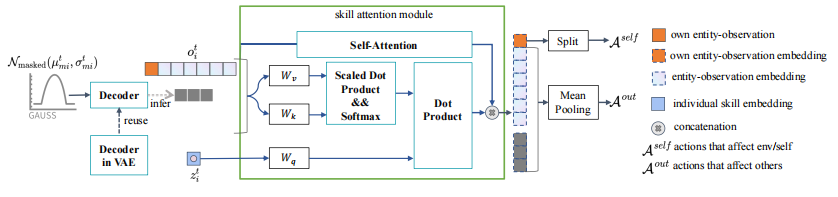
\includegraphics[width=\linewidth]{img_pfe/MA2RL_att_decoder.PNG}
   
    
        \caption{Attentive action decoder. The attentive action decoder utilizes the latent representations of all masked entity-observations to infer the information of masked entities and then applies a skill attention module to obtain the action. (Adapted from \parencite{ma2rl}).}
        \label{fig:ma2rl_att_decoder}
\end{figure}


%---------- MA2E ---------
% While approaches like communication are not always feasible and abstract consensus methods can be lossy, other representation learning techniques like MA2CL or MaskMA are often tightly coupled with the policy network or designed for different objectives like action prediction. To address the need for a more general and modular information inference module,  \parencite{ma2e} proposes the Multi-Agent Masked Auto-Encoder (MA2E). The core idea of MA2E is to use a masked autoencoder to explicitly reconstruct the full trajectories of all agents, conditioned only on the partial trajectory of a single agent. This is achieved by taking the trajectories of all agents, applying agent-level masking (i.e., completely masking out the information of several random agents), and training a Transformer-based autoencoder to reconstruct the original, complete data by minimizing the Mean Squared Error.

% A key differentiator of MA2E is its decoupled, two-stage training process. First, the MA2E module is pre-trained using data from a random policy until it can reliably reconstruct the global information. Then, during the main MARL training, the policy network is trained according to its own objective, while the pre-trained MA2E module is periodically fine-tuned. During decentralized execution, each agent feeds its own local trajectory into its MA2E module to infer a reconstructed global view, which is then used to augment its decision-making. 
% The primary strength of this decoupled design is its modularity and transferability; MA2E can be easily plugged into various existing value-based or policy-based MARL algorithms to significantly boost their performance and sample efficiency. However, the framework has two main limitations: its inference capability degrades when agents are too far apart for their observations to overlap, and its architecture is not designed to easily scale to environments with a varying number of agents.
While approaches like communication are not always feasible and abstract consensus methods can be lossy, other representation learning techniques like MA2CL or MaskMA are often tightly coupled with the policy network or designed for different objectives like action prediction. To address the need for a more general and modular information inference module,
\parencite{ma2e} proposes the Multi-Agent Masked Auto-Encoder (${MA}^2E$). The core idea is to use a masked auto-encoder, built on a Transformer architecture, as a plug-in module for existing CTDE algorithms. During training, the module learns to reconstruct the full trajectories of all agents after having the trajectories of a random subset of agents masked out. This self-supervised task forces the agent to learn a rich latent representation that implicitly contains inferred global information. This representation is then used by the agent's policy for more effective decentralized decision-making. 
The primary strength of ${MA}^2E$ is its ability to significantly improve the sample efficiency and final performance of strong baselines like QMIX, achieving results comparable to having full state information. However, the framework's effectiveness is limited in scenarios where agent observations do not overlap, as there is no information from which to infer the state of distant agents. Furthermore, its architecture is not inherently designed to scale to a dynamically varying number of agents.



%---------- MACKRL ---------

While the CTDE paradigm addresses the non-stationarity of the learning problem, a fundamental limitation persists in many of its implementations, such as COMA \parencite{COMA} or QMIX \parencite{QMIX}. In these frameworks, the requirement for fully decentralized policies during execution often forces agents to ignore potentially useful local information, as acting on it could make their behavior unpredictable to teammates and hinder coordination. To address this, \parencite{mackrl} proposes an alternative paradigm that explicitly leverages common knowledge: information that a group of agents all possess, and all know that they all possess it.


\begin{figure}[h!]
    \begin{minipage}{0.55\textwidth}
       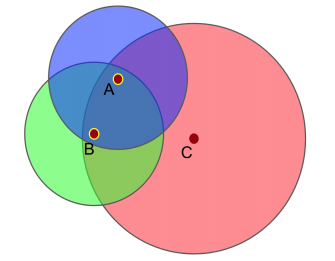
\includegraphics[width=\linewidth]{img_pfe/agent_fov.png}
    \end{minipage}
    \hfill
    \begin{minipage}{0.4\textwidth}

        \captionof{figure}{Three agents and their fields of view (for more details, Annexe~\ref{sec:mackrl_details}). A and B’s locations are common knowledge to A and B as they are within each other’s fields of view. Although C can see A and B, it shares no common knowledge with them. (Adapted from \parencite{mackrl}).}
        \label{fig:agents_fov}
    \end{minipage}

\end{figure}

% \begin{wrapfigure}{r}{0.45\textwidth} % 'r' means float to the right, '0.45\textwidth' is the width
%     \centering
%     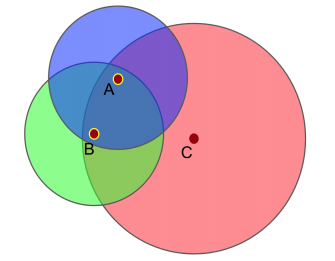
\includegraphics[width=0.4\textwidth]{img_pfe/agent_fov.png}
%     \caption{Three agents and their fields of view (for more details, Annexe~\ref{sec:mackrl_details}). A and B’s locations are common knowledge to A and B as they are within each other’s fields of view. Although C can see A and B, it shares no common knowledge with them. (Adapted from \parencite{mackrl}).}
%     \label{fig:agents_fov}
% \end{wrapfigure}
% \begin{figure}[H]
%     \centering

%     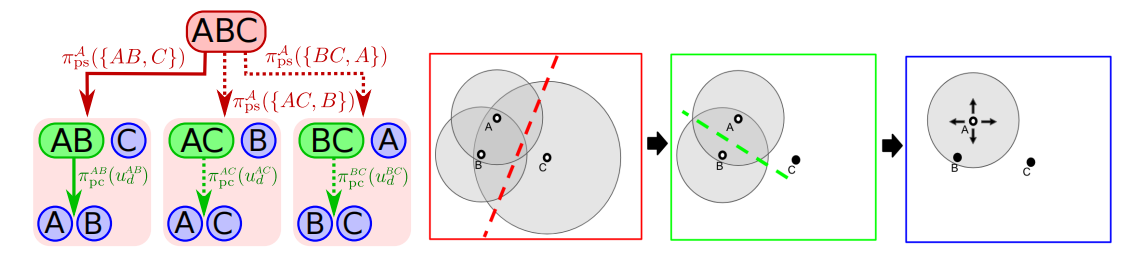
\includegraphics[width=\linewidth]{img_pfe/MACKRL_arch.PNG}
%     % \caption{The hierarchical policy tree of Pairwise MACKRL for three agents. The top-level pair selector chooses a partition (e.g., \{AB, C\}). The pair controller for AB then decides whether to take a joint action or delegate control to the individual agent policies. (Adapted from \parencite{mackrl}).}
%     \caption{
%         An illustration of Pairwise MACKRL.(Adapted from \parencite{mackrl})
%         \texttt{[left]:} the full hierarchy for three agents (dependencies on common knowledge are omitted for clarity). Only solid arrows are computed during decentralised training, while all arrows must be computed recursively during centralised training. 
%         \texttt{[right]:} the (maximally) 3 steps of decentralised sampling from the perspective of agent A.
%         \begin{enumerate}
%             \item Pair selector $\pi_{\text{ps}}^{ABC}$ chooses the partition $\{A,B,C\}$ based on the common knowledge of all agents $\mathcal{I}^{ABC}(\tau^A, \xi) = \emptyset$.
%             \item Based on the common knowledge of pair A and B, $\pi_{\text{pc}}^{AB}(\tau^A, \xi)$, the pair controller $\pi_{\text{pc}}^{AB}$ can either choose a joint action $(u_{\text{env}}^A, u_{\text{env}}^B)$, or delegate to individual controllers by selecting $u_d^{AB}$.
%             \item If delegating, the individual controller $\pi^A$ must select the action $u_{\text{env}}^A$ for the single agent A. All steps can be computed based on A's history $\tau^A$.
%         \end{enumerate}
%     }
%     \label{fig:mackrl_arch}
% \end{figure}

\begin{figure}[H]
    \centering
    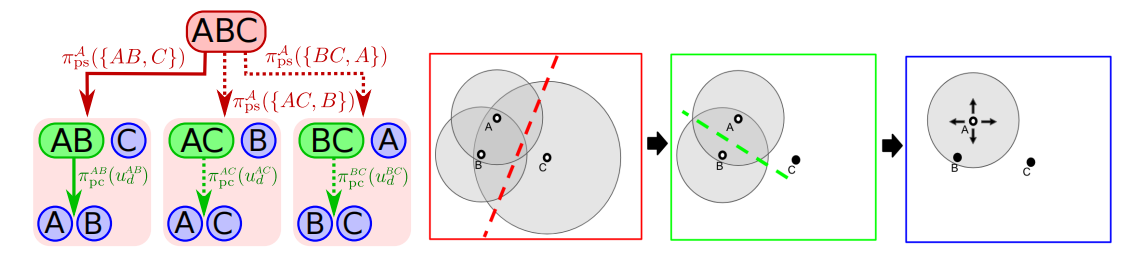
\includegraphics[width=\linewidth]{img_pfe/MACKRL_arch.PNG}
    
    % --- The Caption ---
    % The main caption text goes here.
    \caption{An illustration of Pairwise MACKRL. 
    \texttt{[left]:} the full hierarchy for three agents (dependencies on common knowledge are omitted for clarity). Only solid arrows are computed during decentralised sampling, while all arrows must be computed recursively during centralised training. 
    \texttt{[right]:} the (maximally) 3 steps of decentralised sampling from the perspective of agent A. 
    (Adapted from \parencite{mackrl})}
    \label{fig:mackrl_arch}

    \begin{minipage}{\linewidth}
    \begin{enumerate}
        \item Pair selector $\pi_{\text{ps}}^{ABC}$ chooses the partition $\{A,B,C\}$ based on the common knowledge of all agents $\mathcal{I}^{ABC}(\tau^A, \xi) = \emptyset$.
        \item Based on the common knowledge of pair A and B, $\pi_{\text{pc}}^{AB}(\tau^A, \xi)$, the pair controller $\pi_{\text{pc}}^{AB}$ can either choose a joint action $(u_{\text{env}}^A, u_{\text{env}}^B)$, or delegate to individual controllers by selecting $u_d^{AB}$.
        \item If delegating, the individual controller $\pi^A$ must select the action $u_{\text{env}}^A$ for the single agent A. All steps can be computed based on A's history $\tau^A$.
    \end{enumerate}
    \end{minipage}

\end{figure}

The core idea of Multi-Agent Common Knowledge Reinforcement Learning (MACKRL) is that when common knowledge (for more details, see Annexe~\ref{sec:mackrl_details}) is available, when agents are within each other's line of sight, they can execute complex, coordinated joint actions without the need for communication. The architecture operationalizes this through a hierarchical policy tree, as illustrated in Figure~\ref{fig:mackrl_arch}. Higher levels in this hierarchy learn to coordinate groups of agents by conditioning their joint actions only on their shared common knowledge. If sufficient common knowledge is not available or if coordination is not required, these higher-level controllers can delegate control to lower levels in the tree, which correspond to smaller subgroups or even individual, fully decentralized policies. The entire policy tree is learned end-to-end using a centralized critic, but because all decisions are based on information that each agent can independently deduce (its own local history plus what is common knowledge), the policy can be executed in a fully decentralized manner.

The primary strength of MACKRL is its ability to learn a flexible policy that dynamically switches between tight, joint-action coordination and independent decision-making, based on the information available at any given moment. This allows it to outperform both purely decentralized methods (like IQL) \parencite{Independent_vs_Cooperative_Agents} and other centralized training approaches in specific coordination-heavy benchmarks. However, the framework's main limitations are its scalability and its reliance on a pre-defined common knowledge function. The number of possible agent partitions for the top-level controller grows factorially with the number of agents, making it difficult to scale. Furthermore, the method requires a function to identify when and what common knowledge exists, which may not be available or easy to define in all environments.


% \section{Literature Review}
% \subsection{From Independent to cooperative agents}
% Multi-agent systems can be used to address problems in a variety of domains, including robotics, distributed control, telecommunications, and economics. The complexity of many tasks arising in these domains makes them difficult to solve with pre-programmed agent behaviors. The agents must instead discover a solution on their own, using learning. One of the first papers that addressed the integration of independent agents in a multi-agent system was \cite{IQL}. The author proposed independent policies for each of the agents. The learned decision policy was to be determined by the state-action value function: 
% \begin{equation}
%     Q(x,a) \leftarrow Q(x,a) + \alpha (r+\gamma V(y) - Q(x,a)) 
% \end{equation}
% Using Boltzmann distribution: 
% \begin{equation}
%     p(x,a_i) = \frac{e^{Q(x,a_i)/T}}{\sum _k e^{Q(x,a_k)/T}}
% \end{equation}
% This allows working with a continuous action space, and by adjusting the temperature, we can vary the degree of randomness in action selection. High temperatures lead to more exploratory behavior, while lower temperatures prioritize exploitation. However, IQL still faced many limitations, amongst which are the Partial Observability of the Environment, because when dealing with centralized learning, the agents are only guided by a partially observable environment whose dynamics are in constant change, and the Non-Stationarity of the Environment, due to the fact that independent Algorithms face non-stationarity in Multi-Agent domains due to the violation of the Markovian property in a Markov Decision Process. Thus, convergence is not always guaranteed. 

% In 2017, Foerster et al. introduced a new framework for cooperative agents, "Counterfactual Multi-Agent Policy Gradients" \cite{COMA}. COMA uses a centralized critic (that conditions on true global state $s$ or the joint action-observation histories) to estimate the Q-function and decentralized actors (these are agents receiving feedback from the critic to update their policies) to optimize the agents’ policies. In addition to addressing the challenges of multi-agent credit assignment, it uses a counterfactual baseline that marginalizes a single agent’s action while keeping the other agents’ actions fixed. Agents are in a fully cooperative Multi-agent task $G=\langle \ S, \ U, \ P, \ r, \ Z, \ O, \ n, \gamma \  \rangle$, each of them has a history of action-observation history $\tau ^ a$. Their joint policy induces a state-value function:
% \begin{equation}
%     V^{\pi } (s_t) = E[R_t/s_t]
% \end{equation}
% and an action-state function:
% \begin{equation}
%     Q^{\pi } (s_t, u_t) = E[R_t/s_t, u_t]
% \end{equation}
% The critic's feedback is represented mathematically by an advantage function, comparing the Q-values for current $u^{a}$ to a counterfactual baseline (inspired by reward difference):
% % \begin{equation}
% %     A (s, u) = Q(s, u) - \sum _{u'^{a}} \pi ^{a} (u' ^{a} / \tau ^{a} )  Q(s, (u^{-a} , u' ^{a} )) 
% % \end{equation}

% When dealing with the limitations of IQL (partial observability and non-stationarity), the authors of COMA estimate the advantage of an agent's action by comparing the value of the joint action to counterfactual scenarios where the agent took different actions. All other agents' actions are fixed while computing the advantage function.  A schematic of COMA model during training is shown in Figure C.3 in Appendix C.

% These two papers represented two extremes in the study of cooperation in multi-agent systems and served as an inspiration to many papers aiming to find a middle ground between independent agents and agents working collectively in a centralized setting. Amongst these were:
% \begin{itemize}
%     \item \cite{VDN} which addresses the challenges of cooperative MASs with a single joint reward signal by training individual agents using a novel architecture that decomposes the team value function into agent-wise value functions.
%     \item \cite{QMIX}, which is a value-based method that enables training decentralized policies in a centralized manner by estimating joint action values through a complex non-linear combination of per-agent values based solely on local observations.
%     \item \cite{QTRAN} which introduces a factorization method for multi-agent reinforcement learning tasks in centralized training with a decentralized execution regime.
%     \item \cite{LOLA} which allows each agent to shape the anticipated learning (policies specifically) of the other agents in the environment. This resulted in passive-aggressive behavior from agents. 
% \end{itemize}

% And \cite{PED}, whose authors proposed a value-based deep MARL method that gradually reshapes the rewards in a distributed manner such that the agent’s perception of the equilibrium gears toward optimizing social welfare. The PED-DQN framework can be used in semi-cooperative tasks through decentralized learning with induced peer evaluation. The key challenge in semi-cooperative tasks is selfishness, which is represented by separate reward functions, which often result in the agents choosing non-cooperative actions. 

% Achieving maximum cooperation was quantified by obtaining the optimal policy: 
% \begin{equation}
% \begin{split}
%     \pi ^{*} = & \ (\pi ^{*}(u_1, o_1),  \pi ^{*}(u_2, o_2), ....., \pi ^{*}(u_n, o_n)) \\ 
%      \pi ^{*} = & \ \text{argmax} _{\pi} \sum _a  E[r_a(s,u)]
% \end{split}
% \end{equation}
% The reward update requires that agents' actions become socially optimal ones that maximize cooperation and that they all have access to feedback from peers.

% They proposed reshaping the reward function using a peer evaluation metric, quantified by: 
% \begin{equation}
%     z_a ^t = r_a ^t + \gamma max _u Q_a ^M (o_a ^t , u | \theta ^{M'} _a ) - Q_a ^M (o_a ^t , u_a ^t | \theta ^{M'} _a )
% \end{equation}
% The reshaped reward is: 
% \begin{equation}
% \begin{aligned}
%         \hat{r}_a = & r_a + f_1
%         \\ \hat{r}_a = & r_a +\beta Z_a
%     \\ Z_a = & \frac{1}{|K_a|} \sum _k z_k ^t
% \end{aligned}
% \end{equation}
% The PED-DQN paper uses two neural networks:
% \begin{enumerate}
%     \item \textbf{AQDN: }used to select an action with the maximum Q-value for a given observation, where the target is:
%     \begin{equation}
%         y_a ^A (o'_a, r_a | \theta _a ^{A'}) = r + \gamma max Q^{A} (o'a, u'_a | \theta _a ^{A'}
%     \end{equation}

    
%     \item \textbf{MQDN: } used to calculate the peer evaluation signal, where the target is:
%     \begin{equation}
%         y_a ^M (o'_a, r_a | \theta _a ^{M'}) = \hat{r} + \gamma max Q^{M} (o'_a, u'_a | \theta _a ^{M'})
%     \end{equation}
% \end{enumerate}
% A faster learning rate is used for the MDQN, which updates for quasi-stationary ADQN. The PED-DQN framework, despite giving good results in semi-cooperative settings, still lacked a distributed Peer Evaluation system, assuming agents can be forced to be prosocial and did not weigh on the reputation or the trust of agents. The mechanism of the PED-DQN paper and the Distribution of the peer evaluation scores between agents and their neighbors are shown in Figures C.1 and C.2 in Appendix C.



% In 2019, Zegers et al. introduced in \cite{FCLT} a new mechanism to account for agents' reputations. The idea behind the paper was to develop distributed event-triggered controllers for heterogeneous agents, allowing them to achieve formation control and leader tracking, with resilience to adversarial Byzantine agents. A reputation-based approach is used for the agents to discern between cooperative and Byzantine neighbors, and then selectively disregard Byzantine state information. We will give further insights into this paper in section 2.3.4.


% \subsection{Reward Engineering}
% Reward Engineering is a critical aspect of designing intelligent agents, particularly in complex and dynamic environments. It involves shaping the reward functions that guide the learning process of agents, ensuring that they receive appropriate feedback for their actions. Effective reward engineering can significantly influence the efficiency and effectiveness of learning algorithms, enabling agents to achieve desired outcomes more reliably. By incorporating both extrinsic rewards (based on external goals and tasks) and intrinsic rewards (based on the agent's internal motivations and curiosity), we can create a more efficient and flexible learning framework. 

% Agents in a MAS may be cooperative, competitive, or may exhibit some mixture of these behaviors. Based on the state space, action space, and the goals of the learning, we can either add a reward shaping mechanism or a reward reshaping mechanism. \textbf{Reward Shaping} involves adding additional rewards to the original reward function to guide the agent toward desired behaviors. The primary goal is to make learning more efficient by providing intermediate rewards that help the agent understand which actions are beneficial in the long term. \textbf{Reward Reshaping} refers to modifying the reward function based on the agent's ongoing experience to better reflect the desired outcomes. This approach adjusts the reward signals dynamically as the agent interacts with the environment. The reward function is not static and can be altered during training based on the agent's performance and emerging patterns. Reward Shaping is typically designed and fixed before training begins, while Reward Reshaping occurs during the training process, allowing for dynamic updates to the reward function.

% In both these scenarios, the reshaping function that is added to the base reward function can be modeled through 2 methods: 


% \subsubsection{PBRS (Potential Based Reward Shaping):} 

% This is defined as: 
%     \begin{equation}
%         F(s,s')=\gamma \phi (s') - \phi (s) 
%     \end{equation}
    
%     where $\phi (s)$ is the potential function that returns the potential for state s, and γ is the same discount factor used when updating value function estimates. PBRS has been proven not to
% Alter the optimal policy of a single agent acting in infinite-horizon and finite-horizon MDPs.

% The form of PBRS described above can, however, only represent domain knowledge as a preference for different states, and does not provide any information to the agent regarding spe-
% Specific actions that may be beneficial. PBRS was extended to allow the knowledge
% regarding favorable actions to be included. This extension is called Potential-Based Advice. As
% part of this extension, the potential function is expressed for a state-action pair. This was proposed under two different forms of Potential-Based Advice: 


% \textbf{Look-Ahead Advice:}
% \begin{equation}
%     F(s,a,s',a') = \gamma \phi (s',a') - \phi (s,a)
% \end{equation}

% \textbf{Look-Back Advice:}

% \begin{equation}
%     F(s,a,s',a') =  \phi (s',a') - \gamma ^{-1} \phi (s,a)
% \end{equation}


% In order to guarantee policy invariance for Look-Ahead Advice in single-agent learning scenarios, certain additional criteria must be satisfied. Specifically, how an agent selects actions must be modified so that its policy $\pi$ chooses the action that will maximize the sum of Q-value and potential. However, for the Look-Back Advice, no corresponding proof of policy invariance for a single agent
% learning with Look-Back Advice has been published, although empirical results suggest that Look-Back Advice does not modify the optimal policy in single-agent learning scenarios. 


% \subsubsection{Difference Rewards:} This form of reward shaping is only applicable to cooperative MAS; therefore, only stochastic fully cooperative multi-agent domains are considered in this work. Different rewards are inspired by the intuition that all
% agents in a cooperative MAS should try to contribute to the global utility, and make use of a
% global utility function G.


% A difference reward $D_i$ is a shaped reward signal that aims to quantify each agent’s individual contribution to the system performance in a cooperative MAS:
% \begin{equation}
%     D_s (s_i, a_i) = G(s,a) - G(s_{-i} \cup s_i ^{c} , a_{-i} \cup a_i ^{c})
% \end{equation}

% where $G(s, a)$ is the global system utility, s is the system state, a is the joint action, and $(G(s_{-i} \cup s_i ^{c}, a_{-i} \cup a_i ^{c})$ is the counterfactual which represents the global utility for a theoretical system without the contribution of agent $i$.
% The terms $s_{-i}$ and $a_{-i}$ refer to all the states and actions not involving agent $i$, while $s_i ^{c}$ and $a_i ^{c}$ are fixed states and actions not dependent on agent $i$. Typically, the counterfactual system utility is calculated with agent $i$ removed, or by assuming a default state/action for agent $i$.

% \subsection{Intrinsic Reward}
% Intrinsic rewards, derived from the agent's own experience and introspection, can significantly enhance learning in environments where agents partially cooperate but also pursue individual goals. In such semi-cooperative settings, the introspective reward mechanism allows agents to evaluate and adjust their strategies based on past successes and failures, leading to more adaptive and resilient behavior. This approach fosters a balance between individual learning and collective success, ensuring that agents remain effective and aligned with the overarching objectives of the environment.

% In the next paragraphs, we shed light on multiple works highlighting the use of intrinsic rewards in cooperative, competitive, or coordination games. These studies demonstrate how intrinsic rewards can drive innovation in agent strategies, and enhance cooperation among agents.

% \subsubsection{Cooperation and Reputation Dynamics with RL}


% The goal of this intrinsic reward is achieving stabilizing cooperation in a MAS using a reputation-based approach, by combining two mechanisms: seeding a proportion of the system with fixed agents that steer others towards desired equilibria and introducing intrinsic rewards based on the idea of introspection, inspired from evolutionary game theory (EGT will be defined in the next chapter). It is based on social norms; which are functions that translate how the actions of the parties involved in an interaction, translate into their future reputation (whether agents are seen as good or bad), for example:
% \begin{enumerate}
%     \item \textbf{$0000_2$}: Actions and reputations play no role. 
%     \item \textbf{$0011_2$}: Cooperating with others is always "good" and defecting is always "bad".
%     \item \textbf{$1001_2$}: An agent that cooperates with others with good reputation and defects to those whose reputation is bad is a good agent.
%     \item \textbf{$1011_2$}: Someone is "bad" only if they refuse to cooperate with a good individual.
% \end{enumerate}
% We reshape the reward such as "Agents care about what their policy would do to an agent like themselves."
% \\ The reward becomes:
%     \begin{equation}
%             R_i = \alpha U_i + (1- \alpha) S_i
%     \end{equation}
% with: $U_i$ the payoff in a particular encounter, $S_i$ the payoff they would get if they faced themselves, and $\alpha$ is the level of introspection.

% \subsubsection{Gifting}

% Instead of opponent modeling (like the LOLA model, or using SST (state space vectors) to model the other agents in the environment), gifting allows agents to influence each other's actions, decisions, and strategies without taking the risk of having passive-aggressive behavior during the learning. Gifting extends
% the action space of learning agents in coordination games to allow rewards to be
% transferred among agents. To increase the probability of reaching the prosocial equilibrium in settings with multiple equilibria, This work investigates adding zero-sum gifting actions, so that agents may decide to give some of their rewards to others, preserving the
% total reward of agents.

% For each player, a new set of actions is defined: 

% \begin{equation}
%     \sigma_i : G_1 \ \text{x} \ G_2 \ \text{x} \  \cdots \ \text{x} \  G_N \rightarrow \mathbb{R}
% \end{equation}

% where: 
% \begin{equation}
% \begin{aligned}
%     \forall & g_i \in G_i: g_i \geq 0, 
%     \\ \sigma _i & (g) = -g_i + \frac{1}{N-1} \sum _{j \in -i} g_j
%     \end{aligned}
% \end{equation}
% $g_i$ is the gifting action of agent $i$, $g_j$ the gifting action of its peers $j \in -i$, $g$ denotes the gifting action of all agents, and $\sigma _i$ formulates how the payoff of agent $i$ changes with the gifting actions it receives from its neighbors. The corresponding payoff function for each agent is then: 
% \begin{equation}
%     \Bar{\mu} _i (\Bar{s}) = \mu _i (s) + \sigma _i (g) 
% \end{equation}
% where $\Bar{\mu} _i$ is the payoff function for agent $i$, $\Bar{s} = (s,g)$, $\mu _i (s)$ is the reward the agent $i$ got from executing its own action following its own policy, and $\sigma _i (g)$ accounts for the additional reward or gifts that were sent out by other agents.


% Since $\sum _{i=1} ^N \sigma _i (g) = 0 $, introducing the gifting actions into
% the game does not change the total reward among all agents.

% Figure C.4 in Appendix C shows the technique used in the paper of Seeding agents to promote cooperation. Panel A shows the average cooperation in the last half of the episodes. Panel B shows typical learning trajectories for the population of agents using an efficient social norm. Panel C shows the results for norm 0 $0000_2$: where actions and reputations play no role.

% \subsubsection{Contrastive Introspection:}

% In order to address the issue of long-term credit assignment and the sparse rewards problem, the authors present an approach using offline contrastive learning, which they call Contrastive Introspection. While the agent is training, ConSpec stores the observations’ knowledge in a collection of prototypes summarizing the intermediate states required for success. When an agent arrives at any state that matches one of these prototypes, it gets an additional intrinsic reward to the already established external rewards. This reshaped reward is only taken into consideration if the similarity score exceeds 60$\%$, and if it is the maximum of 6 scores taken in a time window of 6 $(t-3, \cdots,  t, \cdots, t+3)$:
% \begin{equation}
%     \Tilde{r}_{kt} = \lambda \sum ^H _ {i=1} \hat{s}_{ikt} \cdot 1_{\hat{s}_{ikt} = max \{ \hat{s}_{ik, t-3}, \cdots , \hat{s_{ik, t+3}} \} }
% \end{equation}

% ConSpec (as seen in the figure C.5 in the Annex) uses three memory buffers: one for the current mini-batch being trained (B, with a capacity of MB), one for successful episodes (S, with a capacity of MS), and one for failed episodes (F, with a capacity of MF). Each episode consists of T time steps. Our findings indicate that these memory buffers don't need to be very large for ConSpec to function effectively; 16 slots in memory suffice, even for 3D environments. Each buffer stores the raw observations, Ot, encountered by the agent. When a new mini-batch of observations is loaded into B for training, episodes are categorized into successes and failures based on the criteria described in A.1. Observations from these categorized episodes are then stored in S and F in a first-in-first-out (FIFO) manner, with older episodes being overwritten as new ones arrive.




% \subsubsection{Learning from Demonstration}
% This reward relies on the principle of Demonstrator or Expert, which can be used in Reinforcement Learning to encourage faster learning of the agents by giving them access to the state-action pairs that had good quality values. Reward shaping based on this principle can be very beneficial if the reshaping function is well-engineered: 
% \begin{equation}
%     R_F (s,a,s') = R(s,a,s') + F(s,a,s')
% \end{equation}
% The potential function defined for the reward shaping chosen in this work is: 
% \begin{equation}
%     F(s,a,s') = \gamma \phi (s') - Q(s)
% \end{equation}
% This definition was extended by others to include actions and time-steps, allowing for the incorporation of behavioural knowledge that reflects the quality of actions as well
% as states, and allowing the shaping to change over time:
% \begin{equation}
%     F(s,a,t,s',a',t') = \gamma \phi(s',a',t') - \phi (s,a,t)
% \end{equation}
% As in Reinforcement Learning, an agent operating in a Learning-from-demonstration setting looks for a policy π that allows it to execute a certain task. While
% in RL, the agent has a reward signal to evaluate its behavior, this evaluation metric is not present in the Learning from Demonstration setting (similarly for inverse reinforcement learning), and the agent
% must refer to expert demonstrations (sequences of state-action pairs
% {(s0, a0 ), . . . , (sn, an )}) of the task to derive a policy that mimics and generalizes these demonstrations.

% Here, the reshaping function is defined as a Gaussian similarity measure over the state
% space:
% % \begin{equation}
% %     g(s,s^{d} , \sum ) = e^{- \frac{1}{2} (s-s^{d}^{T} \sum ^{-1} (s-s^{d}))}
% % \end{equation}
% By incorporating this expression in the potential function $\phi$, we get:
% % \begin{equation}
% %     \phi (s,a) = max _{s^{d} , a ) g(s,s^{d} , \sum )
% % \end{equation}
% The way the agent collects the experiences is as follows: once the agent's learning starts, at the end of each episode, the Q-value $\hat{q}(s_t , a_t)$ for each state-action in this episode is Monte Carlo estimated until the final time step T :
% \begin{equation}
%     \hat{q}(s_t , a_t) = \sum ^{T} _{k=t} \gamma ^{k-t} r_t
% \end{equation}
% The state-action pairs and their estimated Q values are then stored in a priority queue with the estimated Q-values being the sort key of the queue. If the queue is full (defined by queue size parameter qs), only state-action pairs with a higher estimated Q- value than the smallest in the queue are added (and the smallest are consequently removed). The agent looks into the priority queue (that represents now a queue for the demonstrator experiences) and calculates the potential function:
% \begin{equation}
%     \phi (s,a) = \phi max _{(s^{d} , a)} g(s,s^{d} , \sum ) \hat{q}(s_t , a_t) 
% \end{equation}
% where $\phi$ is a hyper parameter the authors of this paper defined as a scaling factor to control the exploration of the agent.

% \subsubsection{Introspective Learning through queries:} 
% This introspective reward aims to carry out counterfactual reasoning over unrealized events. The authors of the paper introduced an introspection oracle to query the agent on whether there exist states in which the agent would select certain actions. The algorithm uses this data to train and to improve the
% safety of the agent without requiring that such potentially dangerous
% situations be encountered in real life. We shed light on what highlights this reward:
% \begin{itemize}
%     \item Working on a pre-MDP $(D=(S,A,p))$ consisting of a set of states S, set of actions A, and transition probabilities $p(s, a, s′)$.
%     \item $\pi (D)$ is the set of all policies for D. Opt(M) is the subset of $\pi (D)$ containing optimal policies for M. M being the set of all MDPs over D.
%     \item Working with terminal pairs $(S,A)$ instead of terminal states.
%     \item $Pr(X)$ is the set of all well-behaved subsets of $X \in R_n $. Well-behaved subsets $S \times A$ are the ones defined with non-linear function symbols (for example: speed/acceleration).
% \end{itemize}
% We define an introspective oracle for policy $\pi$ as a map:
% \begin{equation}
%     w_{\pi} : Pr (S \times A) \rightarrow \{ \bot \} + S
% \end{equation}
% with $\bot$ indicates an error, or in other terms, the pair was not found in time. If $w_{\pi} (U)=s$ then the pair is found, where $U$ refers to the property of the pair (state, action). We query the state
% $s = w(U_i)$, and if it is found, then $(w_{\pi} (U), \pi(w_{\pi} (U))$ is in $U$. The examples gathered are inserted into the replay buffer as terminal.


% These introspective rewards can all be helpful for the agents for faster learning and faster convergence. However, in the scenario of the gifting model, agents can become greedy and selfish with passive-aggressive behavior. The cooperation and reputation dynamics paper introduced social norms to the environment, which can limit its dynamics (in an Atari game, prey-predator..). The introspective learning through queries takes into consideration the future mistakes that an agent can make and helps them avoid them by making those states terminal and ending the episode. Finally, the contrastive reward took into account the state-action pairs with the highest values as prototypes for the agents to learn from. Although both these methods, in addition to the learning from demonstration method, have led to good results in simulations, they were not very efficient in a semi-cooperative prey-predator scenario. 


% \subsection{Byzantine agents}

% We start by defining the \textbf{Byzantine Generals' Problem}: A number of generals are attacking a fortress. The generals must decide as a group and agree on a common decision: whether to attack or retreat 
% $\rightarrow$ If only a few generals attack, it is worse than a coordinated attack or a coordinated retreat. 

% There are two types of Byzantine agents, and each one has a type of attack that compromises the decision-making process:
% \begin{enumerate}
%     \item \textbf{Byzantine Agents type I: } remains in the mobile network, where it can delay or corrupt information communicated to its neighbors (Feeding false information like the generals who vote to attack but will retreat).
%     \item \textbf{Byzantine Agents type II: } Abandons the mobile network while communicating true or no state information about itself (like generals who will eventually attack but maybe with different allies). 
% \end{enumerate}


% \begin{figure}[hbt!]
%   \centering
%   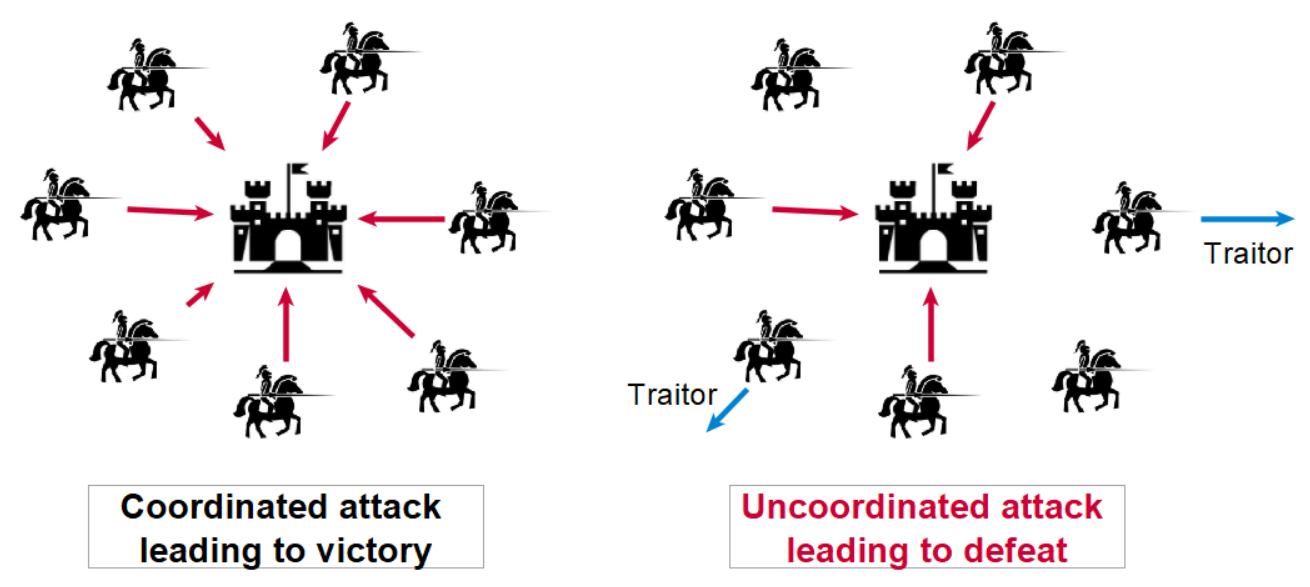
\includegraphics[width=0.8\textwidth]{images_pfe/1_xJGKNqJVrkFVtZ6NggwHbw.png}
%   \caption{A representation of the Byzantine agents.}
% \end{figure}
% \FloatBarrier

% As we already stated in the previous section, the inspiration behind this work is to develop distributed event-triggered controllers for heterogeneous agents, allowing them to achieve formation control and leader tracking, with resilience to adversarial Byzantine agents. A reputation-based approach is used for the agents to discern between cooperative and Byzantine neighbors, and then selectively disregard Byzantine state information. We define:
% \begin{itemize}
%     \item $B: [0, \infty [ \rightarrow 2 ^ \nu$ : time-varying set of Byzantine agents.
%     \item $C: [0, \infty [ \rightarrow 2 ^ \nu$ : time-varying set of Cooperative agents.
% \end{itemize}
% This leads to $ B(t) \cap C(t) = \emptyset $ and $B(t) \cup C(t) = \nu $ (the leader not included).
% \vspace*{0.1cm}
% The agent's dynamics were modeled as an uncertain non-linear model for the agent's velocity: 
% \begin{equation}
%     \dot{x}_i(t) = f_i (x_i(t)) + g_i (x_i(t)) u_i(t) + d_i(t), \forall \ i  \in  \mathlarger{\nu} \cup  \{ 0 \}
% \end{equation}
% Where: 
% \begin{itemize}
% \item \textbf{$f_i$:} $R^n \rightarrow R^n$: \textbf{uncertain drift dynamics}: describe the long-term behavior or trend in an agent's motion that can be influenced by uncertain disturbances.
%     \item \textbf{$g_i$:} $R^n \rightarrow R^{n*m}$: \textbf{known control effectiveness matrix}: describes how the control inputs for each agent affect the entire system's state. 
%     \item \textbf{$u_i$:} $[0, \infty ) \rightarrow R^m$: \textbf{control input}.
%     \item \textbf{$d_i$:} $[0, \infty ) \rightarrow R^n$: \textbf{exogenous disturbance} for agent i: the external influence that affects the behavior/dynamics/state of the agent. 
% \end{itemize}
% As for the controllers' development, the authors proposed a model based on 4 steps: 
% \begin{enumerate}
%     \item Building a trust model
%     \item Building a reputation model
%     \item Study of an edge weight policy
%     \item Building an event-triggered control mechanism for each agent
% \end{enumerate}
% However, this mechanism faces certain limitations; the need for a ground truth, the need for an accurate state estimation of all agents, and the lack of distinction between Byzantine agents and Cooperative agents in the absence of the ground truth.


\section*{Conclusion}
This review of the state-of-the-art has traced the evolution of cooperative MARL algorithms, from foundational value-decomposition networks like VDN and QMIX to more advanced representation learning frameworks designed to overcome partial observability. While methods like COLA and MACKRL introduce clever ways to share or align agent information, they can be limited by abstract representations or restrictive assumptions. More recent approaches based on masked auto-encoding, particularly ${MA}^2E$, have shown great promise by learning to reconstruct a global view from local observations. However, as identified in our analysis, ${MA}^2E$'s reliance on a policy-agnostic, random masking strategy represents a key limitation, creating a disconnect between the representation learning task and the agent's actual learning progress. It is this specific gap that necessitates a masking strategy dynamically informed by the MARL training process itself, which motivates the novel contribution presented in the next chapter.



\chapter{Our Contribution : A Learning-Informed Masking Framework for Multi-Agent Representation Learning}


% \section*{Introduction : From General Inference to Policy-Relevant Representation}

% In this chapter, we present the findings from our experiments and provide an analysis of the results. We will explore the performance of the baseline algorithms and the impact of various modifications and enhancements on these algorithms. The chapter is structured to discuss the results obtained from different experimental setups, analyze the implications of these results, and interpret their significance in the context of our research objectives. Our primary focus is on understanding how the introduced methods affect the stability, convergence, and overall effectiveness of the techniques we presented in Chapter 3 in our given MARL environment.

% The previous chapter established the Multi-Agent Masked Auto-Encoder (${MA}^2E$) as a powerful method for inferring global information from local observations \parencite{ma2e}. While its self-supervised objective is effective, a critical analysis of its training methodology reveals a key limitation: the use of a policy-agnostic, random masking strategy during the fine-tuning phase.

% This chapter argues that for optimal performance, the self-supervised reconstruction task must be dynamically aligned with the agents' evolving policies. We introduce a novel framework that scores agent performance in real-time and uses this information to intelligently mask the most uncertain or \textit{poorly learning} agents. This forces the ${MA}^2E$'s representational power to focus where it is needed most, creating a more efficient and effective learning curriculum.
\section*{Introduction }
The previous chapter established the Multi-Agent Masked Auto-Encoder (${MA}^2E$ ) \parencite{ma2e} as a powerful method for inferring global information from local observations. The central thesis of our work is that to create the most effective environmental representations, the inference process itself should be guided by information from the agents' own training dynamics.

A critical analysis of the original ${MA}^2E$  methodology reveals a key limitation in this regard: use of a policy-independent and randomly applied masking strategy during  training masked auto encoder . This random approach creates a disconnect between the self-supervised reconstruction task and the primary reinforcement learning objective.

This chapter argues that for optimal performance, these two tasks must be dynamically aligned. We introduce a novel framework that scores agent performance in real-time and uses this information to intelligently mask the most uncertain or \textit{poorly learning} agents. This forces the ${MA}^2E$ 's representational power to focus where it is needed most, creating a more efficient and effective learning curriculum.
% \subsection{Preliminaries: The Masked Auto-Encoder}

\section{The Masked Auto-Encoder}
\label{section:mae_original}
% At the core of our approach is the Masked Auto-Encoder (MAE), a powerful self-supervised learning model that has demonstrated remarkable success in representation learning, particularly in computer vision \parencite{maskedautoencoder}. An MAE learns robust latent representations by solving a challenging self-supervised task: reconstructing a complete input signal from a heavily corrupted, partial version.
\begin{figure}[H] 
    \centering
    % Box for the image
        % \includegraphics[width=\linewidth]
         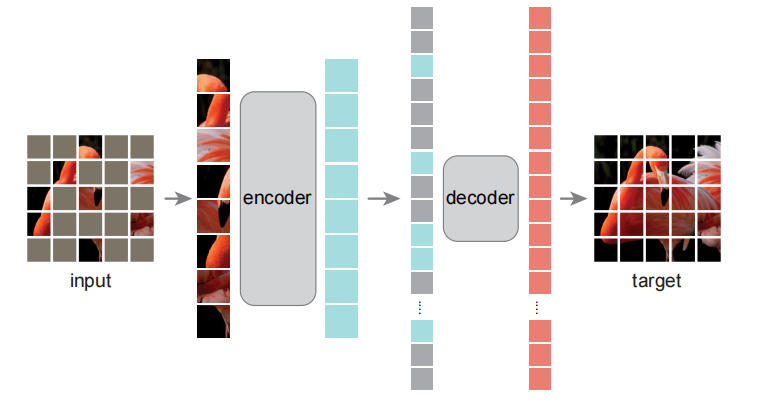
\includegraphics[width=0.8\linewidth]{img_pfe/mae_original.PNG}
   
    
        \caption{MAE architecture. (Adapted from \parencite{maskedautoencoder}).}
        \label{fig:mae_original}
\end{figure}
% \subsection{Preliminaries: A Detailed Examination of the Masked Auto-Encoder}
At the core of our approach is the Masked Auto-Encoder (${MAE}$ )  \parencite{maskedautoencoder}, a self-supervised learning paradigm that represents a significant shift in representation learning. Unlike contrastive methods that learn by comparing different views of data, MAE learns by solving a generative, reconstruction-based task. The core philosophy is to corrupt a signal and train a model to restore it, compelling the model to internalize the data's underlying structure and semantics. This section provides a detailed, step-by-step deconstruction of the ${MAE}$  framework.

% \subsubsection*{The MAE Pipeline: From Corrupted Input to Semantic Representation}
\subsection*{The ${MA}E$  Pipeline :[Figure \ref{fig:mae_original}]}
% The MAE process can be understood as a sequence of carefully designed steps, each with a specific purpose that contributes to the model's overall effectiveness and efficiency.

\paragraph{Input tokenization} The process begins with input tokenization, where the image is deconstructed into a sequence of discrete elements. The image is divided into a regular grid of non-overlapping patches (e.g., 16x16 pixels), each flattened into a vector and linearly projected to a fixed dimension, creating \textit{visual tokens}. A linear embedding layer performs this transformation, with learnable positional embeddings added to retain spatial information. This step is crucial as it converts the image into a sequence format compatible with Transformer architectures while avoiding redundancy from overlapping regions.
% \paragraph{Aggressive random masking}
\paragraph{Random masking} Next, aggressive random masking is applied, where a large, random subset of tokens (often 75\% or more) is discarded. This high masking ratio is essential to  prevents the model from relying on low-level spatial redundancy and instead forces it to develop a high-level understanding of the image to reconstruct missing parts effectively. The masking is performed via uniform random sampling, leaving only a small fraction of tokens visible.

\paragraph{Asymmetric encoder} The asymmetric encoder, a Vision Transformer (ViT) \parencite{vit}, processes only the unmasked tokens. 
% This design choice is key to MAE's efficiency: since the encoder operates on just 25\% of the data (for a 75\% masking ratio), it dramatically reduces computational cost while still learning rich semantic representations. 
The encoder employs multi-head self-attention to model relationships between tokens, building context-aware features, as illustrated in Figure \ref{fig:vit}.
% \paragraph{Lightweight decoder}
\begin{figure}[H]
    \centering
    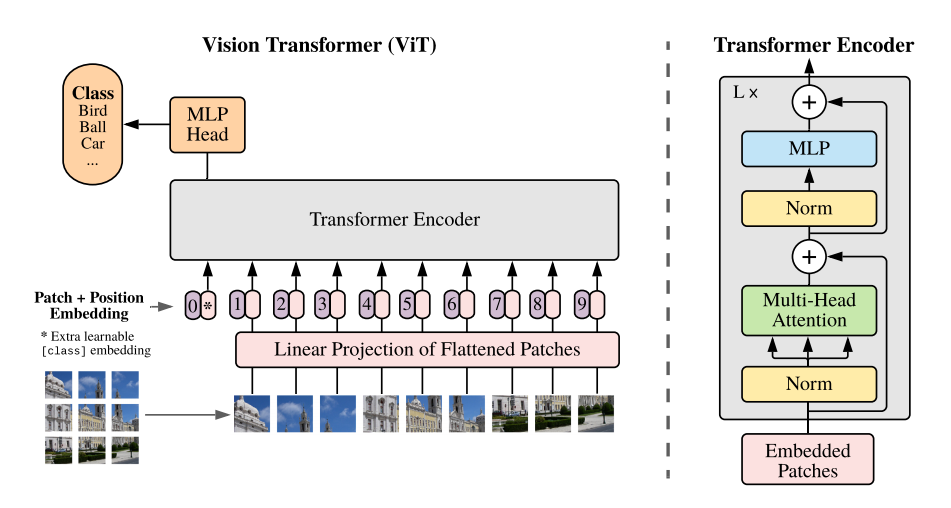
\includegraphics[width=0.8\linewidth]{img_pfe/vit.PNG}
    \caption{Model overview of \textbf{ViT}. We split an image into fixed-size patches, linearly embed each of them, add position embeddings, and feed the resulting sequence of vectors to a standard Transformer encoder. In order to perform classification, we use the standard approach of adding an extra learnable \textit{classification token} to the sequence. The illustration of the Transformer encoder was inspired by \parencite{attention_is_all_you_need}. (Adapted from \parencite{vit})}
    \label{fig:vit}
\end{figure}
% \begin{figure}[H]
%     % \centering
%     \begin{minipage}{0.7\textwidth}
        
%     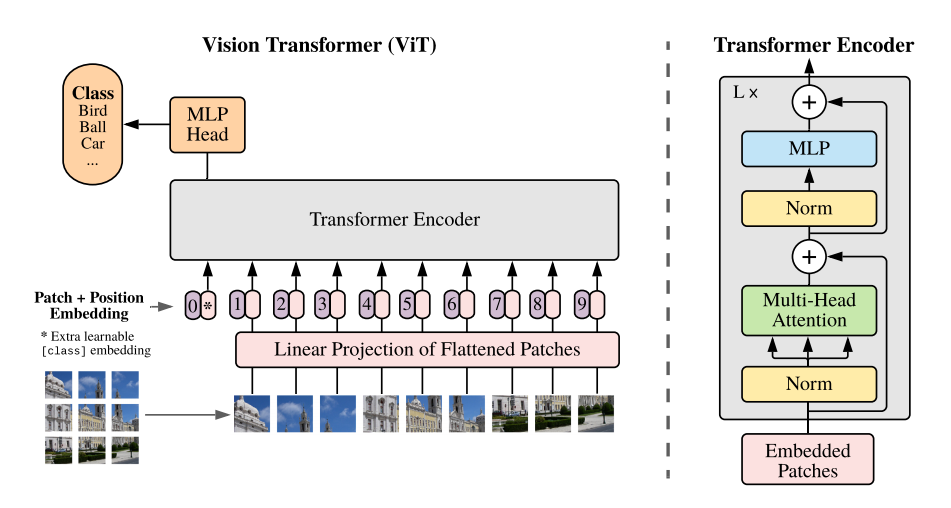
\includegraphics[width=\linewidth]{img_pfe/vit.PNG}
%     \end{minipage}
%     \hspace{0.05\textwidth} 
%     \begin{minipage}{0.2\textwidth}
        
%                 \captionof{figure}{Model overview of \textbf{ViT}. We split an image into fixed-size patches, linearly embed each of them, add position embeddings, and feed the resulting sequence of vectors to a standard Transformer encoder. In order to perform classification, we use the standard approach of adding an extra learnable “classification token” to the sequence. The illustration of the Transformer encoder was inspired by \parencite{attention_is_all_you_need}. (Adapted from \parencite{vit})}
%         \label{fig:vit}
%     \end{minipage}
% \end{figure}
\paragraph{Decoder} 
% A lightweight decoder then reconstructs the full image from the encoded tokens.
a decoder then reconstructs the full image from the encoded tokens.
The decoder takes the encoder's output and reintroduces learnable \texttt{[MASK]} tokens as placeholders for missing patches, each with their correct positional embeddings.Unlike the encoder, the decoder is shallow and computationally inexpensive, as its role is not deep representation learning but rather upsampling high-level features back into pixel space.

\paragraph{Reconstruction loss} Finally, the reconstruction loss provides the learning signal. The model predicts pixel values for masked patches, and the loss \textbf{(Mean Squared Error Equation \eqref{eq:mae_loss})} is computed only on these masked regions, not on visible patches. This ensures that the model focuses on inferring missing information, reinforcing meaningful latent representations. 
The loss function for an image $x$ with masked indices $M$ is:
\begin{equation}
    \label{eq:mae_loss}
    L = \frac{1}{|M|} \sum_{i \in M} \left\| x_i - \hat{x}_i \right\|^2
\end{equation}
where $x_i$ is the original pixel vector for the $i$-th patch and $\hat{x}_i$ is the reconstructed vector.

\subsection*{Key Innovations and Rationale Behind MAE’s Design}
The MAE framework introduces several critical innovations that contribute to its efficiency and effectiveness in self-supervised learning.

\paragraph{High masking ratio} First, the high masking ratio (often 75\% or higher) is a deliberate choice to create a sufficiently challenging pretext task. Natural images contain significant spatial redundancy, meaning that with a low masking ratio, a model could exploit local correlations to reconstruct missing patches without truly understanding high-level semantics. By aggressively masking most of the input, MAE forces the model to develop robust, abstract representations that capture object structure and scene composition.

\paragraph{Asymmetric encoder-decoder architecture} Second, the asymmetric encoder-decoder architecture is central to MAE’s computational efficiency. The encoder, which is the most resource-intensive component due to its deep self-attention layers, processes only the small subset of visible tokens. This reduces both memory usage and training time significantly.
% —by a factor of 3x or more compared to processing the full image. 
Meanwhile, the  decoder handles reconstruction, ensuring that the bulk of the learning occurs in the encoder’s high-level feature space rather than in pixel-level prediction.

\paragraph{Selective reconstruction loss} Another key aspect is the selective reconstruction loss, computed exclusively on masked patches. This design ensures that the model does not simply memorize visible patches but instead learns to infer missing content based on contextual understanding. By focusing the loss on masked regions, LI-MAE encourages the model to develop semantically rich representations that generalize well to downstream tasks.

\paragraph{Tokenization and positional embedding} The tokenization and positional embedding strategy also plays a crucial role. By dividing the image into non-overlapping patches and embedding them with positional information, MAE maintains spatial relationships while converting the input into a sequence suitable for Transformer processing. This approach avoids the inefficiencies of convolutional sliding windows while preserving structural awareness.

% In summary, MAE’s success stems from its carefully balanced design: aggressive masking forces meaningful learning, the asymmetric architecture ensures efficiency, and the reconstruction loss sharpens the model’s ability to reason about missing information. These principles collectively enable MAE to learn powerful visual representations in a scalable, self-supervised manner.

% The MAE architecture and methodology can be broken down into the following key components:

% \begin{description}
%     \item[Input Patching and Masking] The input (e.g., an image) is first divided into a sequence of non-overlapping patches. A large portion of these patches, often as high as 75\%, are randomly removed or ``masked.'' This high masking ratio is crucial, as it makes the reconstruction task non-trivial and prevents the model from simply extrapolating from adjacent patches, forcing it to learn a more holistic understanding of the data.
    
%     \item[Asymmetric Encoder-Decoder Architecture] MAE employs an asymmetric design to process this masked data efficiently.
%     \begin{itemize}
%         \item \textbf{The Encoder:} A high-capacity encoder, typically a Vision Transformer (ViT)\parencite{vit}, operates only on the small subset of visible, unmasked patches. By not processing the masked portions, the computational load during training is significantly reduced (e.g., by 3x or more).
%         \item \textbf{The Decoder:} A separate, lightweight decoder is tasked with the reconstruction. Its input consists of the latent representation of the visible patches (from the encoder) combined with a series of shared, learned ``mask tokens'' that serve as placeholders for the missing patches.
%     \end{itemize}
    
%     \item[Reconstruction Task] The lightweight decoder processes this full sequence of encoded patches and mask tokens to predict the pixel values for only the masked portions of the original input. The model is trained by minimizing a reconstruction loss, such as Mean Squared Error (MSE), between its predictions and the ground-truth values of the masked patches.
% \end{description}

% By learning to predict the missing content from a limited context, the encoder is forced to develop a semantically rich latent representation without requiring any explicit labels, making it a powerful foundation for downstream tasks.
% \section{Architectural Framework}

\section{Architectural Framework}
Our approach is designed as a methodological enhancement to the existing ${MA}^2E$ architecture \parencite{ma2e}. While we do not alter the core network components (the agent's backbone network and the ${MA}^2E$'s Transformer-based auto-encoder), we introduce a novel information flow during the training phase that fundamentally changes how the system learns. This section details the architectural components and the integration of our learning-guided masking mechanism.

The overall framework, as depicted conceptually in  the original ${MA}^2E$  paper \parencite{ma2e}, is composed of two primary parts for each agent:
\begin{description}
    \item[Individual Agent Network (Backbone)] Each agent $i$ possesses its own individual network, which serves as the backbone for the chosen MARL algorithm (e.g., QMIX\parencite{QMIX}(As discussed in Section~\ref{subsec:ctde}  Chapter~\ref{chap:sota}  )). This network, typically a recurrent model like a GRU, is responsible for processing the agent's local action-observation history $h_i$ to produce a hidden state. During the training of our framework, this network also outputs the essential learning signals (such as the Temporal Difference error) that are required to evaluate the agent's performance.
    
    % \item[MA2E Module (Inference Engine)] A shared Transformer-based masked auto-encoder (For more details see Section~\ref{section:mae_original} ) is used by the agents , its role is to take agent trajectories as input and reconstruct them from a masked version. The goal of this module is learning to generate a latent representation that contains global context inferred from partial information.
  \item[$LI-{MA}^2E$  Module ]  Is an inference engine designed to be integrated into existing MARL frameworks \parencite{ma2e}. Its architecture, illustrated in Figure \ref{fig:ma2e_architecture}, is a Transformer-based auto-encoder specifically adapted for multi-agent trajectory data. This section provides a detailed breakdown of each layer in the $LI-{MA}^2E$  pipeline.



% \paragraph{Input Trajectories Layer}
% The foundational data unit for MA2E is not a single state or observation, but a batch of multi-agent trajectories, denoted as $\tau_{t-T+1:t}^{1:n}$. This input, which represents the observation-action histories for all $n$ agents over a time window of length $T$, is structured from the replay buffer into the required sequence format. The reason for using trajectories is that this sequential data contains the essential temporal context required for the model to infer the complex behaviors, intents, and correlations between agents over time.
\begin{itemize}
    \item \textbf{Input Trajectories Layer} The foundational data unit for ${MA}E$ is not a single state but a batch of multi-agent trajectories, $\tau_{t-T+1:t}^{1:n}$, representing the observation-action histories for all $n$ agents over a time window of length $T$. Using full trajectories is crucial because this sequential data contains the essential temporal context required for the model to infer the complex behaviors and intents of other agents.
    \item \textbf{Masking Layer} This layer receives the full sequence of agent trajectories and applies the core masking strategy. As shown in the diagram by the red  \texttt{[X]} markers, the trajectories of a randomly selected subset of $k$ agents are entirely masked out, producing a corrupted sequence where some agents' data is visible and some is hidden. This agent-level masking is a critical design choice tailored to MARL. Unlike masking random patches in an image, masking entire agent trajectories forces the model to solve a more challenging and relevant problem: inferring the complete state and behavior of one agent based on the behavior of others. This directly encourages the model to learn the complex inter-agent dynamics necessary for effective coordination.
    % \item \textbf{Positional Encoding Layer} To provide the necessary sequential context to the permutation-invariant Transformer, this layer adds learnable positional vectors to each token after an initial embedding projection. In MA2E, this is particularly important because the input has two dimensions of order: time and agent ID. Therefore, the positional encoding must capture both, allowing the model to distinguish between, for example, \textit{agent 1 at time t} and \textit{agent 2 at time t}. The paper's\parencite{ma2e} ablation studies confirm that using encodings that consider both agent and time dimensions yields significantly better performance.
    \item \textbf{Positional Encoding Layer}  To provide sequential context to the permutation-invariant Transformer, this layer adds learnable positional vectors to each token after   an initial embedding projection. Since the input has two dimensions of order \textit{time} and \textit{agent ID} the encoding must capture both to distinguish between different agents at different times, for example, \textit{agent 1 at time t} and \textit{agent 2 at time t}. Ablation studies confirm this dual-dimensional encoding is critical for performance \parencite{ma2e}.
    % , enriching the tokens with the structural information needed for the model to succeed.
    \item \textbf{Transformer Encoder Block} Following an asymmetric design for efficiency, a powerful encoder processes only the small, visible subset of unmasked agent trajectories. By applying stacked Multi-Head Attention layers to this sparse input, it learns the complex relationships between agents while using a fraction of the computational resources. Its output is a sequence of latent vectors representing a deep, context-aware encoding of the visible data.
    \item  \textbf{Transformer Decoder Block} The lightweight decoder (shallower and narrower) receives a full sequence of tokens, which is constructed by combining the latent vectors for the visible trajectories (from the encoder) and learnable \texttt{[MASK]} tokens as placeholders for the agents whose trajectories were masked out. Its purpose is not to learn a deep semantic representation, but to perform the final reconstruction task by using the context from the encoded visible tokens to predict the features of the masked tokens. Its output is a full sequence of reconstructed trajectory vectors, $\tilde{\tau}_{t-T+1:t}^{1:n}$.
    \item \textbf{Reconstructed Trajectories (Output Layer)} A final linear projection layer takes the output vectors from the decoder and maps them back to the original dimension of the trajectory data ($o_t^i, u_t^i$). This produces the final reconstructed trajectories for all agents. This output is then compared against the original ground-truth trajectories using a \textbf{Mean Squared Error  loss } function, which in turn generates the gradients that drive the entire learning process.

    
\end{itemize}
% \paragraph{Input Trajectories Layer} The foundational data unit for MA2E is not a single state but a batch of multi-agent trajectories, $\tau_{t-T+1:t}^{1:n}$, representing the observation-action histories for all $n$ agents over a time window of length $T$. Using full trajectories is crucial because this sequential data contains the essential temporal context required for the model to infer the complex behaviors and intents of other agents.
% \paragraph{Masking Layer}
% This layer receives the full sequence of agent trajectories and applies the core masking strategy. As shown in the diagram by the red 'X' markers, the trajectories of a randomly selected subset of $k$ agents are entirely masked out, producing a corrupted sequence where some agents' data is visible and some is hidden. This agent-level masking is a critical design choice tailored to MARL. Unlike masking random patches in an image, masking entire agent trajectories forces the model to solve a more challenging and relevant problem: inferring the complete state and behavior of one agent based on the behavior of others. This directly encourages the model to learn the complex inter-agent dynamics necessary for effective coordination.

% \paragraph{Positional Encoding Layer}
% To provide the necessary sequential context to the permutation-invariant Transformer, this layer adds learnable positional vectors to each token after an initial embedding projection. In MA2E, this is particularly important because the input has two dimensions of order: time and agent ID. Therefore, the positional encoding must capture both, allowing the model to distinguish between, for example, ``agent 1 at time t'' and ``agent 2 at time t''. The paper's ablation studies confirm that using encodings that consider both agent and time dimensions yields significantly better performance, enriching the tokens with the structural information needed for the model to succeed.

% \paragraph{Transformer Encoder Block}
% Following the asymmetric design of the original MAE, a powerful encoder, composed of stacked Multi-Head Attention (MHA) and feed-forward layers, processes only the sequence of tokens corresponding to the visible (unmasked) agent trajectories. The MHA mechanism allows each visible trajectory token to attend to every other visible trajectory token, learning the complex relationships between the agents whose information is available. The rationale for this design is efficiency; by operating on only a small subset of the total data, the most computationally intensive part of the model runs significantly faster and uses less memory, making the entire training process more tractable. The output is a sequence of latent vectors representing a deep, context-aware encoding of the visible trajectories.



 % Its purpose is to use the encoded context from the visible trajectories to efficiently reconstruct the features of the masked ones, outputting a complete sequence of trajectory vectors.

    \begin{figure}[H]
    \centering
      
    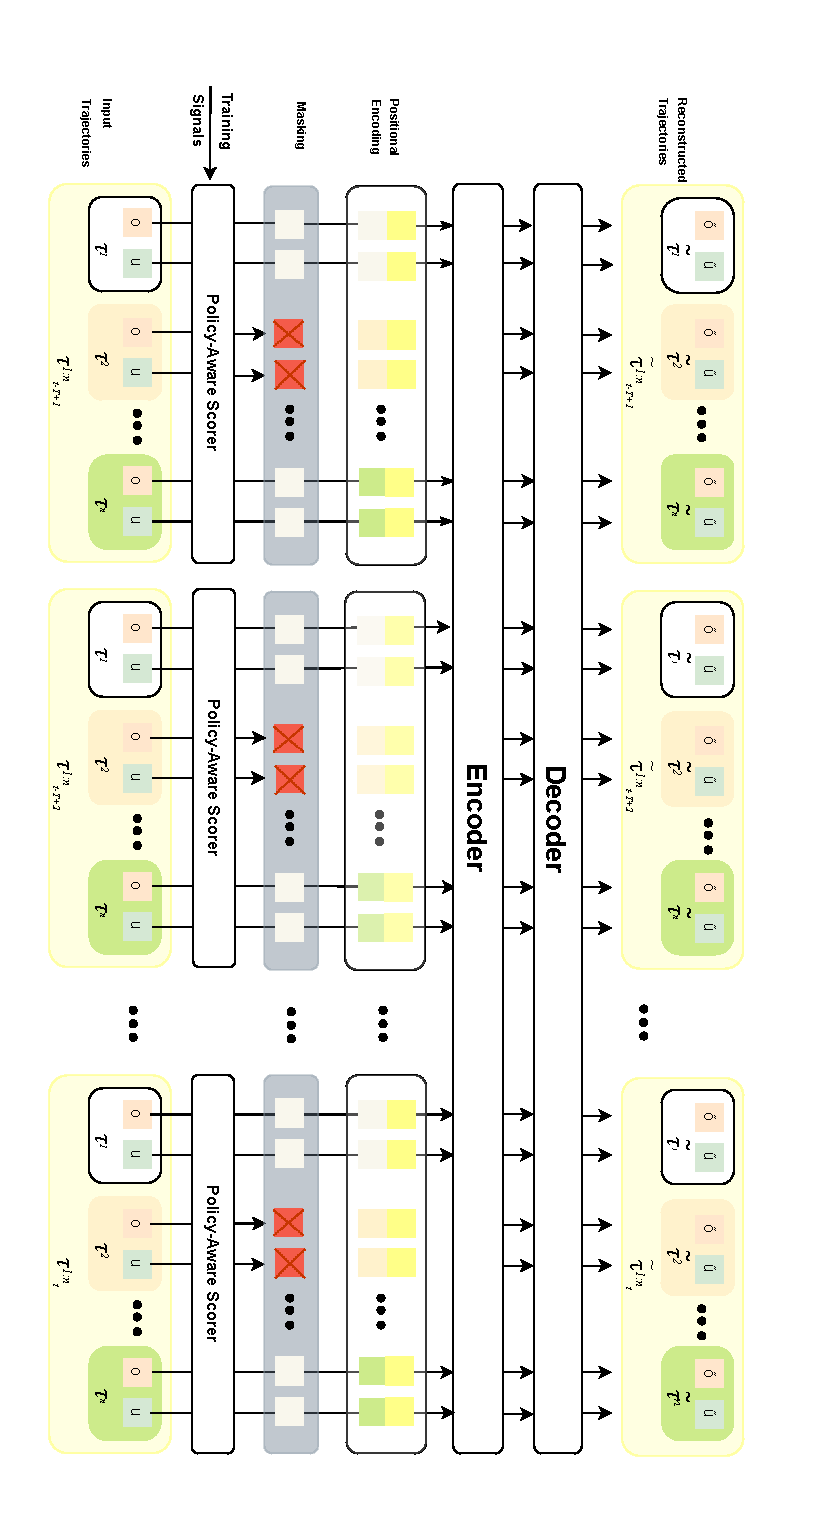
\includegraphics[angle=90, width=0.99\linewidth]{img_pfe/li-mae_this.pdf}
  \caption{The architecture of our proposed \textbf{Learning-Informed Masking ($LI-{MA}^2E$)} framework. Building upon the baseline ${MA}^2E$ , our approach introduces a Policy-Aware Scorer module. During the fine-tuning phase, this module receives training signals (e.g., TD-errors) from the main MARL algorithm and uses them to identify \textit{poorly performing agents}. It then generates a \textit{control signal} that guides the Masking Layer to prioritize masking these specific agents,  forcing the  $LI-{MA}^2E$ module to focus its representational power on reconstructing the trajectories of the most uncertain or poorly performing agents, ensuring the self-supervised task remains Harmonious with the primary reinforcement learning objective.}
    \label{fig:ma2e_architecture}
\end{figure}

\end{description}
% \begin{figure}[htbp]
% \centering

% \caption{The architecture of MA²E. During centralized training, MA²E identifies poor learning agents from all agents' trajectories $\tau_1^1, \tau_1^2, \ldots, \tau_1^k$ and learns to help them improve. The positional encoding is applied considering both the time and the agent information. During decentralized execution, trajectories of poor learning agents are improved while good agents maintain their performance.}
% \label{fig:ma2e_architecture}
% \end{figure}

% \begin{figure}[H]
%     % \centering
%     \begin{minipage}{0.7\textwidth}
        
%     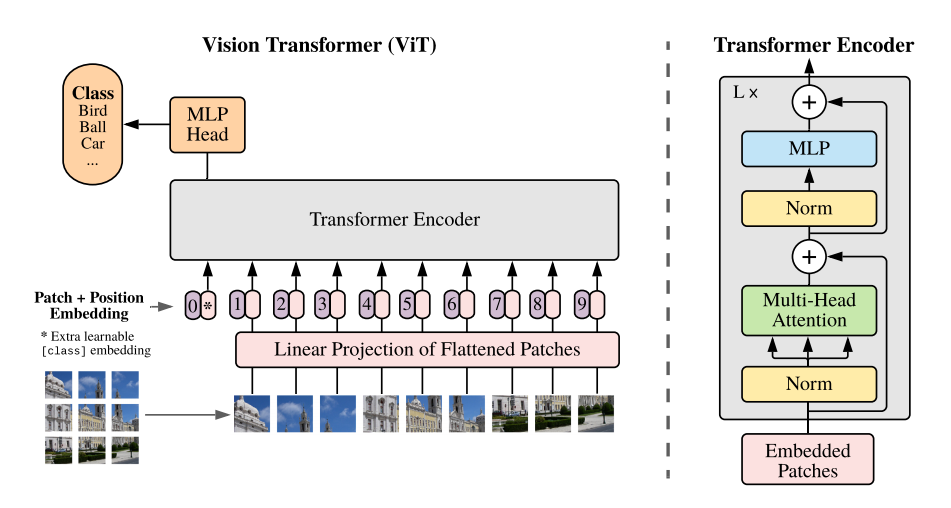
\includegraphics[width=\linewidth]{img_pfe/vit.PNG}
%     \end{minipage}
%     \hspace{0.05\textwidth} 
%     \begin{minipage}{0.2\textwidth}
        
%                 \captionof{figure}{Model overview of \textbf{ViT}. We split an image into fixed-size patches, linearly embed each of them, add position embeddings, and feed the resulting sequence of vectors to a standard Transformer encoder. In order to perform classification, we use the standard approach of adding an extra learnable “classification token” to the sequence. The illustration of the Transformer encoder was inspired by \parencite{attention_is_all_you_need}. (Adapted from \parencite{vit})}
%         \label{fig:vit}
%     \end{minipage}
% \end{figure}

\section{Methodology}
The core of our contribution is a redesigned training methodology that establishes a complementary relationship between the reinforcement learning objective and the self-supervised representation learning task.
% This section provides a detailed, step-by-step explanation of this protocol, following the structure of the original MA2E framework \parencite{kang2025ma2e} upon which it builds.

\subsection{Masking Strategy}
Our framework utilizes a distinct masking strategy for each of its two training phases.
\begin{description}
    \item[During Pre-training (Random Masking)] In the initial phase, we employ the baseline random agent-level masking. The goal is to learn a generalized world model from data collected by a random policy. A subset of $k$ agents is chosen uniformly at random, and their entire observation-action trajectories are masked.
    % This policy-agnostic approach is ideal for this stage as it forces the model to learn general representations without any task-specific bias.
    
    
    \item[During Fine-tuning (Learning-Informed Masking )]  During the main policy training, we replace random masking with  Learning-Informed Masking. Instead of random selection, we identify the \textit{poorly learning} agents within a training batch by using the \textbf{Temporal Difference (TD) error} from the backbone MARL algorithm as a direct performance metric. Agents associated with higher TD-errors are assigned a higher score for being masked. This makes the $LI-{MA}^2E$ focus its representational power on the most uncertain and challenging aspects of the cooperative task.
\end{description}

% \subsection{Core Architecture}
% % The MA2E module itself is a Transformer-based auto-encoder, as illustrated in Figure~\ref{fig:ma2e_architecture}. Following an embedding layer, the input trajectories are processed by a masking layer and a positional encoding layer. This encoding is critical as it must capture the two dimensions of order in the data: the time step and the agent ID. The architecture is asymmetric, with a deep encoder that processes only the visible trajectories and a lightweight decoder that reconstructs the full set from the encoder's output and learnable \texttt{[MASK]} tokens. The encoder and decoder are both built from standard Transformer blocks using Multi-Head Attention (MHA) and feedforward networks.

\subsection{Integration with the Backbone Agent}
The $LI-{MA}^2E$ module is integrated into each agent's individual network to augment its local perception with inferred global context.
\begin{description}
    \item[Parallel Processing] An agent's local history is fed into both its backbone network (e.g., a GRU) and the shared $LI-{MA}^2E$ module.
    \item[Information Fusion via Self-Attention] The reconstructed trajectories from the $LI-{MA}^2E$, $\tilde{\tau}_{1:n}$, are passed to a self-attention mechanism. This layer allows the agent to learn a context-aware summary of the global state by weighing the importance of its teammates' inferred situations relative to its own. The agent's own reconstructed trajectory $\tilde{\tau}_i$ acts as the query, while the others act as keys and values.
    \item[Aggregation] The output of the self-attention layer is then aggregated (e.g., via concatenation) with the hidden state from the agent's backbone network. This fused vector, combining private knowledge with relevant global context, is passed to an aggregation network that produces the final \textit{Q-value} or \textit{policy}.
\end{description}

\subsection{The Training Process:}
The training process is carefully divided into two distinct stages to ensure stability and effectiveness.
\begin{description}
    \item[Stage 1: ${LI-{MA}^2E}$ Pre-training] Before policy learning, the ${LI-{MA}^2E}$ module is trained in isolation on data from a random policy, using the random masking strategy. This is crucial for stability, as it ensures the ${LI-{MA}^2E}$ is already a competent inference engine before the policy begins to rely on it. The module is trained to minimize the Mean Squared Error (MSE) reconstruction loss until it falls below a predefined threshold:
    \begin{equation}
        \label{eq:ma2e_loss}
        L_{\text{LI-${MA}^2E$}} = \frac{1}{nT} \sum_{t=1}^{T} \sum_{i=1}^{n} \left( \tau_t^i - \tilde{\tau}_t^i \right)^2
    \end{equation}
    
    \item[Stage 2: Policy Training and  Fine-tuning] After pre-training, the main MARL training begins. The agent's policy is updated for a set number of steps using the chosen algorithm (e.g., QMIX). This process generates the TD-errors that our Masking  layer  uses to create its  policy-aware mask. The LI-${MA}^2E$  module is then periodically fine-tuned using the same MSE loss, but on data corrupted by this new adaptive mask. This periodic schedule balances stability and adaptability, allowing the policy to learn from a consistent world model while still enabling that model to improve over time based on the agent's learning progress.
\end{description}
% \subsection{Integration with Policy-Aware Masking}
% The novelty of our approach lies in the synergistic integration of these two components. Instead of the MA2E module operating with a random, policy-agnostic masking strategy, its masking process is directly informed by the learning progress of the backbone MARL algorithm. This creates a feedback loop where the reinforcement learning task guides the self-supervised representation learning task.

% The architectural components and data flow are as follows:
% \begin{description}
%     \item[Backbone Individual Network] This is the primary policy or value network for each agent (e.g., a DRQN).
%     \begin{description}
%         \item[What it does:] It processes the agent's local action-observation history to produce a hidden state encoding the agent's private belief.
%         \item[Why we use it:] It serves as the foundation for the agent's decision-making and, crucially for our method, it is the source of the training signals (like TD-error) that quantify the agent's learning progress.
%     \end{description}
    
%     \item[Adaptive Curriculum Masking (ACM) Module] This is the core of our novel contribution.
%     \begin{description}
%         \item[What it does:] This module takes the learning signals from the backbone network as input. It then computes a ``poorly learning'' score for each agent and generates a mask where agents with higher scores are more likely to be masked.
%         \item[Why we use it:] It replaces the policy-agnostic random masking with an intelligent, policy-aware curriculum. This ensures that the MA2E's representational power is focused on the agents that need the most assistance.
%     \end{description}
    
%     \item[MA2E Inference Engine] The standard MA2E auto-encoder.
%     \begin{description}
%         \item[What it does:] The encoder takes the visible (unmasked) agent trajectories as input and produces a latent representation. The decoder then attempts to reconstruct the masked trajectories.
%         \item[Why we use it:] It is the engine that performs the self-supervised learning, generating a rich representation that contains inferred global information.
%     \end{description}
    
%     \item[Aggregation Network] A final network layer that fuses information.
%     \begin{description}
%         \item[What it does:] It takes as input both the hidden state from the agent's backbone network and the latent representation from the MA2E encoder. It then aggregates these two sources of information.
%         \item[Why we use it:] It allows the agent to combine its private knowledge with the inferred global context, creating a final, comprehensive representation for decision-making.
%     \end{description}
% \end{description}

% The training process, which will be detailed in the subsequent sections, is briefly composed of a pre-training phase with random masking to establish a general world model, followed by a fine-tuning phase where our policy-aware ACM module is employed to create a targeted learning curriculum.
\subsection{The Critical Role of Pre-training in Representation Learning}
A core methodological choice in our framework is the use of a two-phases during  training : a self-supervised pre-training phase followed by a task-specific fine-tuning phase. This \textit{pre-train, fine-tune} paradigm is not an arbitrary design choice, but a foundational principle in modern machine learning that is essential for achieving stable and high-performing models. This section justifies the necessity of the pre-training stage .

The primary reason for using pre-training is to decouple initial representation learning from downstream task learning, thereby preventing unstable learning dynamics. Attempting to train a MARL policy and  MAE concurrently from scratch creates a vicious cycle : the MARL policy, initially random, generates poor-quality data, which prevents the world model from learning a useful representation. In turn, this inaccurate world model provides noisy and misleading information back to the policy, destabilizing its learning process. Pre-training breaks this cycle by first developing a competent and generalized world model, which then provides a robust foundation for the policy to learn from.

The power of this paradigm was first demonstrated conclusively in the field of \ac{NLP} with the introduction of \ac{BERT} \parencite{bert_pretraining_deep_bidirectional_transformers_language_understanding}. The \ac{BERT} paper revolutionized NLP by showing that a deep Transformer model could be pre-trained on a simple, self-supervised objective : predicting randomly masked words from a massive unlabeled text corpus. By learning to solve this \textit{Masked Language Model} task, the model was forced to develop a deep, contextual understanding of language. The key finding was that this pre-trained model could then be adapted to a wide variety of downstream tasks (e.g., question answering, sentiment analysis) by adding just one task-specific layer and fine-tuning the entire network Figure~\ref{fig:bert_architecture}. This established that a  pre-trained representation could serve as a powerful and transferable foundation, solidifying the \textit{pre-train, fine-tune}  strategy as a dominant approach in the field.
\begin{figure}[H]
    \centering
   
        
    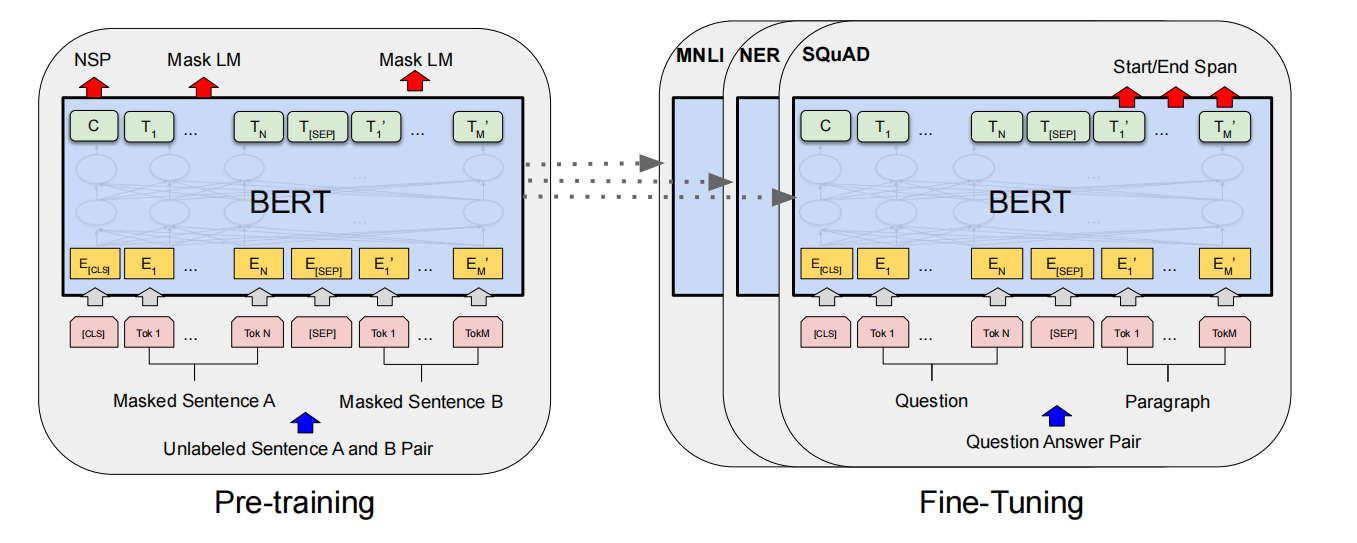
\includegraphics[width= 0.9\linewidth]{img_pfe/bert.png}
 
  
                \caption{Overall pre-training and fine-tuning procedures for BERT. Apart from output layers, the same architectures are used in both pre-training and fine-tuning. The same pre-trained model parameters are used to initialize models for different down-stream tasks. During fine-tuning, all parameters are fine-tuned. \texttt{[CLS]} is a special
symbol added in front of every input example, and \texttt{[SEP]} is a special separator token (e.g. separating questions/answers).(Adapted from \parencite{bert_pretraining_deep_bidirectional_transformers_language_understanding})}
        \label{fig:bert_architecture}
\end{figure}
Building directly on this success, the \textbf{BEiT (Bidirectional Encoder representation from Image Transformers)} \parencite{beit_bert_pretraining_image_transformers} paper successfully translated this paradigm to the domain of computer vision . The authors explicitly state their motivation as adapting the BERT-style pre-training for image data. To overcome the challenge that images lack a natural vocabulary like text, BEiT introduced a two-stage process: first, an image is \textit{tokenized} into a sequence of discrete visual tokens using a separate auto-encoder. Then, during pre-training, the model is given a version of the image where some patches are masked, and its objective is to predict the correct visual tokens for those masked patches. BEiT's success demonstrated that the core principle of learning a representation through a masked reconstruction task is not limited to language but is a powerful and generalizable strategy. This work reinforces the idea that establishing a robust foundational model through a self-supervised pre-training phase is a standard and necessary step before proceeding to task-specific fine-tuning.


More recently, this pre-training philosophy has been directly and successfully applied to the domain of \textit{sequential decision-making and reinforcement learning}. The \textbf{Masked Decision Prediction (MaskDP)} framework illustrated in Figure ~\ref{fig:MaskDP} \parencite{mae_scalable_generalizable_decision_making}
explicitly uses a masked auto-encoder, pre-trained on state-action trajectories, to create a scalable and generalizable agent . The central idea is that by pre-training the model to reconstruct randomly masked states and actions from a trajectory, it learns a rich understanding of the environment's dynamics. The authors \parencite{mae_scalable_generalizable_decision_making} demonstrate that this single, pre-trained model can then be applied to various downstream tasks, such as \textit{goal-reaching} or \textit{offline RL} , often in a \textit{zero-shot manner}. This powerfully reinforces the core idea that a pre-training phase on a self-supervised reconstruction task is a highly effective strategy for learning a versatile and transferable world model that can be efficiently adapted for specific decision-making problems.
\begin{figure}[H]
    \centering
   
        
    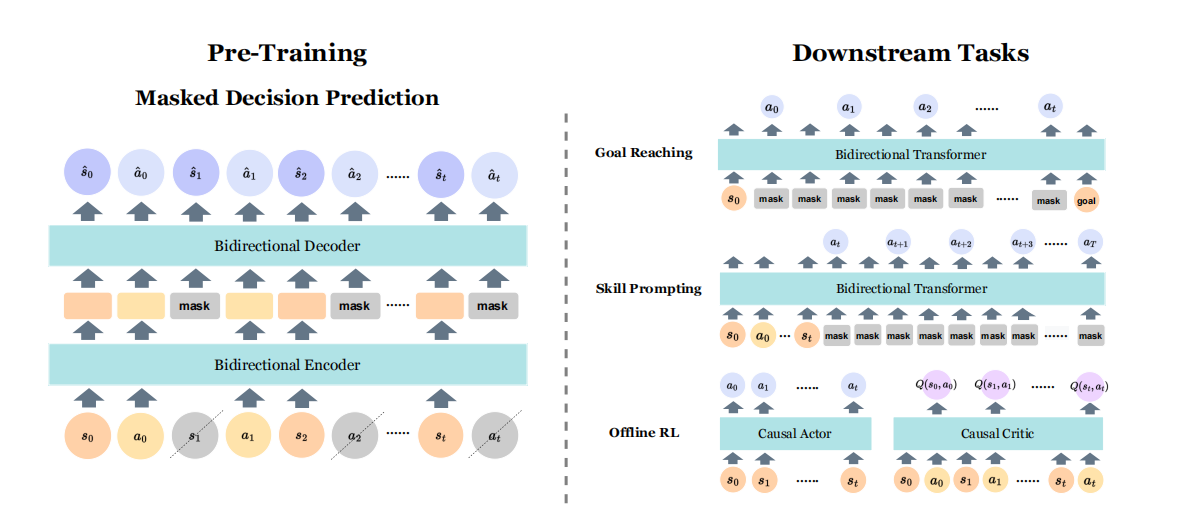
\includegraphics[width= 0.9\linewidth]{img_pfe/mae_Scalable_and_Generalizable_Decision_Making.PNG}
 
  
                \caption{Illustration of MaskDP. During \textit{pretraining} stage, we perform the masked token prediction task. And after pretraining, the model can be deployed to various downstream tasks using different mask patterns.(Adapted from \parencite{mae_scalable_generalizable_decision_making})}
        \label{fig:MaskDP}
\end{figure}
In recent years, this pre-training philosophy has been directly and successfully applied to the domain of sequential decision-making and reinforcement learning. The work on \textbf{Masked World Models (MWM) for visual control} \parencite{masked_world_models_visual_control} explicitly argues for \textit{decoupling visual representation learning} from \textit{dynamics learning }. The authors \parencite{masked_world_models_visual_control}  contend that training a single model end-to-end for both objectives creates a detrimental trade-off that prevents the model from capturing the \textit{fine-grained visual details} necessary for complex robotic control . Their solution is a two-stage process where an auto-encoder is first trained on a masked reconstruction task to learn a rich visual representation. Only after this representation is learned is a separate latent dynamics model trained on top of these powerful, pre-trained features . This explicit separation prevents the dynamics learning objective from interfering with the visual learning objective, providing strong evidence that a pre-trained visual model offers a superior foundation for subsequent RL tasks .


Similarly, the \textbf{Masked Trajectory Models (MTM)  framework} \parencite{masked_trajectory_models_prediction_representation_control} showcases the extreme 	flexibility that a pre-trained model can offer . MTM pre-trains a single, general-purpose model on a unified task: reconstructing randomly incomplete state-action trajectories. The key insight is that a single model, pre-trained in this way, can be used for a multitude of downstream tasks without any retraining. By simply changing the masking pattern at inference time, the model can function as an offline RL agent, a forward dynamics model, or an inverse dynamics model. This powerfully illustrates that a robust, pre-trained representation of environment dynamics is not only transferable but can also be highly versatile, accelerating and in some cases even replacing the need for specialized downstream models. Together, these works provide strong support  that a two-stage protocol, beginning with a self-supervised pre-training phase to learn a robust world model, is a critical component for achieving stable, efficient, and high-performing results in complex decision-making domains.

\section*{Conclusion}

This chapter detailed our primary contribution :\textbf{the Learning-Informed Masking Framework ($LI-{MA}^2E$)} . We began by deconstructing the principles of the Masked Auto-Encoder, establishing it as a powerful tool for self-supervised representation learning. We then presented our novel framework, which introduces a \textbf{Policy-Aware Scorer} module that integrates directly with the backbone MARL algorithm. The core of our methodology is a two-phase training process: an initial pre-training stage with random masking to build a general world model, followed by a fine-tuning stage where our \textbf{Learning-Informed Masking} uses signals like the TD-error to focus the MAE's representational power on the most uncertain agents. By creating this direct link between the reinforcement learning objective and the self-supervised reconstruction task, our framework ensures the two remain aligned, fostering a more efficient and effective learning curriculum. Having formally defined this new methodology, the next chapter will provide a comprehensive empirical validation of its performance.

Having formally defined this new methodology, a critical design question remains:\textbf{What is the most effective metric for identifying a 'poorly performing' agent in a way that best serves the representation learning task?}  The next chapter will address this directly, beginning with a methodical investigation into several candidate scoring functions before presenting a comprehensive empirical validation of the final, optimized framework.
% \chapter{Experiments and Results}


% % \newpage

% \section*{Introduction}
% \label{sec:introduction}

% This chapter presents a comprehensive empirical evaluation of our proposed Learning-Informed Masking Framework. As established in the previous chapter, our work builds upon the Multi-Agent Masked Auto-Encoder (MA2E) architecture, a powerful method for inferring global information from local observations. However, we identified a key limitation in the original MA2E: its reliance on a policy-agnostic, random masking strategy. This approach creates a disconnect between the self-supervised reconstruction task and the primary reinforcement learning objective.

% The central thesis of our work is that for optimal performance, these two tasks must be dynamically aligned. This chapter aims to empirically validate our core hypothesis: that using an agent's own training dynamics to guide the representational learning process yields a more efficient and effective learning curriculum. Specifically, we will test whether our proposed Learning-Informed Masking—which leverages the Temporal Difference (TD) error to focus the autoencoder's attention on the most uncertain agents—yields superior performance over the original random masking approach.

% To validate this, we will benchmark our framework directly against the baseline original MA2E. This focused comparison is designed to isolate and measure the impact of our intelligent masking strategy. The experiments are conducted on the challenging StarCraft Multi-Agent Challenge (SMAC) \parencite{smac},
% % and its more demanding successor, SMACv2 \parencite{smacv2},
% to test the limits of coordination and generalization under partial observability.
\chapter{Experiments and Results}

\section*{Introduction}
\label{sec:introduction_ch5} 

This chapter provides a comprehensive empirical validation of our proposed Learning-Informed Masking Framework ($LI-{MA}^2E$). The primary objective is to demonstrate its superiority over the baseline ${MA}^2E$ framework, which utilizes a random masking strategy. To achieve this, we conduct a series of rigorous experiments on a diverse suite of challenging scenarios from the StarCraft Multi-Agent Challenge (SMAC).

The chapter is structured to present a complete scientific narrative. We begin by detailing our methodical investigation into several candidate scoring functions, showing the iterative process that led to the selection of our final, most effective approach: Adaptive Mean TD-Error Thresholding. Following this, we present a comprehensive performance evaluation of this optimized framework, structured to answer three core research questions regarding its effectiveness in \textit{task completion} (via win rate), its ability to produce \textit{high-quality policies} (via mean test return), and the underlying \textit{learning dynamics} that drive its success (via TD-error).

Ultimately, this chapter will provide robust, multi-faceted evidence to support our central thesis that a learning-informed masking curriculum is superior to a random one in complex, cooperative multi-agent tasks.

\section{Experimental Details}
In this section, we introduce the environments used in the experiments, the baseline algorithm, and the hyperparameters and computational resources. Experiments are carried out on an NVIDIA RTX A5000 GPU (24.6\,GB VRAM) and an Intel\textregistered\ Xeon\textregistered\ W-2235 CPU (6-core, 12-thread), with 32\,$\mathrm{GB}$ DDR4 RAM and CUDA 12.4 support. All algorithms are implemented based on the open-source framework pymarl2\footnote{From: \url{https://github.com/hijkzzz/pymarl2}}  \parencite{pymarl2}, which is an augmented version of pymarl\footnote{From: \url{https://github.com/oxwhirl/pymarl}}. Both are licensed under Apache License 2.0. 
 All the experiments are conducted during a minimum $1 \times 10^6$ time steps.
 %, and we report \textit{the average win rates} with the shaded standard error random seeds.

\subsection{Environments}
\subsubsection{SMAC}

The StarCraft Multi-Agent Challenge (SMAC) \parencite{smac} is one of the benchmarks widely utilized in research to evaluate MARL algorithms. In SMAC, units from the strategy video game StarCraft engage in combat in diverse scenarios. The objective is for multiple agents to collaborate to defeat the enemy forces. The scenarios are categorized by difficulty  Table~\ref{tab:smac_senarios_part1} and Table~\ref{tab:smac_senarios_part2}.

\noindent\textbf{Note:} The objective in all scenarios in Table~\ref{tab:smac_scenarios_used} is to defeat all enemy units by employing the strategy noted in the \textbf{Type} column.

\begin{table}[H]
\centering

\renewcommand{\arraystretch}{1.6} 

\begin{tabular}{ccccc}
\hline
\textbf{Scenario} & \textbf{Difficulty} & \textbf{Ally Units} & \textbf{Enemy Units} & \textbf{Primary Micro-Trick} \\
\hline
3s\_vs\_3z & EASY & 3 Stalkers & 3 Zealots & Kiting \\
\hline
3s\_vs\_4z & MEDIUM & 3 Stalkers & 4 Zealots & Kiting \\
\hline
3s\_vs\_5z & HARD & 3 Stalkers & 5 Zealots & Kiting \\
\hline
3m & EASY & 3 Marines & 3 Marines & Focus Fire \\
\hline
8m & MEDIUM & 8 Marines & 8 Marines & Focus Fire \\
\hline
\end{tabular}
\caption{A detailed description of the SMAC scenarios used in the experiment.}
\label{tab:smac_scenarios_used}
\end{table}
% \subsubsection{SMACv2}

% SMACv2 \parencite{smacv2}  was proposed to address the shortcomings of the original SMAC, particularly its lack of stochasticity and meaningful partial observability (for more details \parencite{smacv2_review}). Therefore, SMACv2 differs from SMAC in three main aspects:

% \begin{enumerate}
%     \item \textbf{Random Unit Composition:} In SMAC, the units in each matchup are fixed, whereas in SMACv2, different unit types are randomly generated for each episode based on probabilities.
%     \item \textbf{Probabilistic Observation:} In SMACv2, if one agent observes an enemy, other nearby agents may not immediately identify the same enemy, even if it is within their observation range. This contrasts with SMAC, where an enemy observed by one agent is simultaneously visible to all other agents.
%     \item \textbf{Randomized Spawn Locations:} The starting positions for units are randomized and determined by one of two types: \texttt{surround} or \texttt{reflect}. \texttt{surround} places allied units in a formation encircling the enemy, while \texttt{reflect} involves a head-on confrontation.

% \begin{figure}[h]
%     \centering
   
        
%     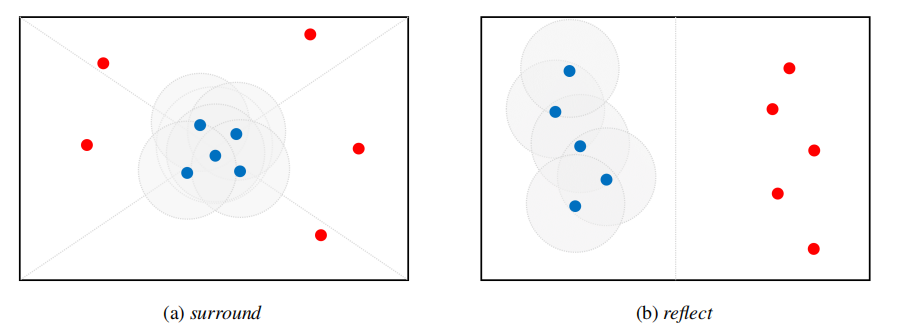
\includegraphics[width= 0.7\linewidth]{img_pfe/start_pos_smacv2.PNG}
 
  
%                 \caption{Two different types of start positions in SMACv2.(Adapted from \parencite{ma2e})}
%         \label{fig:start_pos_smacv2}
% \end{figure}
    
% \end{enumerate}

\subsection{Baseline Algorithm}

Our experiments are designed to isolate the impact of our Learning-Informed masking strategy. Therefore, the baseline for all comparisons is the \textbf{original ${MA}^2E$ architecture}, which utilizes a \textbf{random masking strategy} during training. Both our proposed framework and the baseline are integrated into the \textbf{\ac{QMIX}} algorithm.


\subsection{Hyperparameters}

To ensure a controlled and fair comparison, our proposed framework (\textbf{QMIX + $LI-{MA}^2E$}) and the baseline (\textbf{QMIX + ${MA}^2E$}) share the same core network architecture and hyperparameters. The parameters for the QMIX backbone algorithm are listed in Table \ref{tab:qmix_hyperparams}, and the parameters for the $LI-{MA}^2E$ and ${MA}^2E$ module are listed in Table \ref{tab:ma2e_hyperparams}. These values were used for all experimental runs.

\begin{table}[H]
\centering

\renewcommand{\arraystretch}{1.5} 
\begin{tabular}{lc} 
\hline
\textbf{Hyperparameter} & \textbf{Value} \\
\hline 
Optimizer & Adam \\
Learning Rate (lr) & 0.001 \\
Batch Size & 128 \\
Replay Buffer Size & 1000 \\
Discount Factor ($\gamma$) & 0.99 \\
TD-Lambda ($\lambda$) & 0.6 \\
Epsilon Anneal Steps & 100000 \\
RNN Hidden Dimension & 128 \\
QMIX Mixing Embedding Dimension & 32 \\
\hline
\end{tabular}
\caption{Hyperparameters for the QMIX Backbone Algorithm.}
\label{tab:qmix_hyperparams}
\end{table}

\begin{table}[H]
\centering

\renewcommand{\arraystretch}{1.5} 
\begin{tabular}{lc} 
\hline
\textbf{Hyperparameter} & \textbf{Value} \\
\hline 
Input Trajectory Length & 5 \\
Batch Size & 32 \\
Input Embedding Dimension & 24 \\
Number of Attention Heads & 4 \\
Number of Encoder Layers & 3 \\
Number of Decoder Layers & 2 \\
Steps for Fine-Tuning & 500 \\
Pre-training Threshold & 0.015 \\
\hline
\end{tabular}
\caption{Hyperparameters for the \textbf{$LI-{MA}^2E$} and \textbf{${MA}^2E$} Module.}
\label{tab:ma2e_hyperparams}
\end{table}
\section{Developing the Learning-Informed Masking Score}
% \section{Comparative Analysis of Agent Scoring Methods}
\label{sec:scoring_methods}

The core of our \textbf{$LI-{MA}^2E$ framework} is the ability to intelligently mask \textit{poorly performing} agents. However, defining \textit{poor performance} is not simple. To determine the most effective metric, we designed and empirically evaluated several candidate scoring methodologies, each with a unique theoretical motivation. This section details our investigation into these scoring methods, their underlying rationales, their limitations, and the results that led to our final design choice.
\subsection{Method 1: TD-error with Exponential Moving Average (EMA)}
\label{subsec:ema_method}


Our initial approach to identifying poorly performing agents was to track their long-term performance stability. We chose the TD-error as the fundamental metric for this task. The TD-error, generated during the training of the backbone algorithm, represents the "surprise" or prediction error of an agent's value function for a given transition. 

\paragraph{why \ac{TD} error as metric  ?} 
TD error quantifies the difference between the predicted value of a state-action pair and a better-informed estimate based on the next state:

\begin{equation}
    \delta_t = 
    \underbrace{\left(r_{t+1} + \gamma \max_{a'} Q(s_{t+1}, a')\right)}_{\text{TD target}} 
    - Q(s_t, a_t)
    \label{eq:td_error}
\end{equation}

\begin{itemize}
    \item $r_{t+1}$: The immediate reward received after taking action $a_t$ in state $s_t$.
    \item $\gamma$: The discount factor, controlling the weight of future rewards.
    \item $Q(s_{t+1}, a')$: The estimated value of the next state $s_{t+1}$ under action $a'$, over which we take the maximum (greedy choice) to estimate the best possible future return.
    \item TD target: represents a better-informed estimate of the return assuming the agent acts optimally from $s_{t+1}$ onward.

\end{itemize}

A high absolute TD error ($|\delta_t|$) indicates that the agent's current estimate is significantly inaccurate: highlighting a weakness in its value function and suggesting that this region of the state-action space reflects \textit{poor learning progress}.



Our first hypothesis was that smoothing this error signal over time using an \ac{EMA} would provide a stable measure of an agent's overall learning quality, filtering out noisy, single-step errors. The \ac{EMA} is updated recursively, giving more weight to recent errors while still retaining information from the past. The formula is:
\begin{equation}
    \text{EMA}_t = \alpha \cdot |\delta_t| + (1 - \alpha) \cdot \text{EMA}_{t-1}
    \label{eq:ema}
\end{equation}
where $\alpha$ is the decay rate, determining the balance between new and historical errors.

\paragraph{Implementation}
The implementation is tightly coupled with the overall training loop. Our framework follows a periodic fine-tuning schedule: the QMIX agent policies are trained multiple times, and during this time, all TD errors generated are continuously collected and stored in a large buffer, paired with their respective agent IDs. When it is time to fine-tune the MAE module, a mini-batch of these historical errors is sampled from the buffer. For each agent, the mean of its TD errors within that batch is calculated. This local mean is then used to update the agent's global EMA score. Finally, a softmax function is applied to the EMA scores of all agents to create a probability distribution from which agents are sampled for masking.

\paragraph{Investigating the Role of Historical Data}
A critical parameter in an \ac{EMA} is the decay rate, $\alpha$, which controls the balance between historical data and recent updates. To understand this trade-off, our QMIX + $LI-{MA}^2E$ model was tested with two distinct values for $\alpha$:
\begin{itemize}
\item \textbf{$\alpha=0.1$:} This gives low weight to recent errors and high weight to the existing average. The resulting score is very stable and slow to change, reflecting an agent's long-term historical performance.
\item \textbf{$\alpha=0.9$:} This gives high weight to recent errors, making the score much more reactive and sensitive to an agent's current struggles.
\end{itemize}

\paragraph{Results and Limitations}
\begin{figure}[h]
\centering
\subfloat[\label{fig:ema_0.9} EMA with ($\alpha=0.9$)]{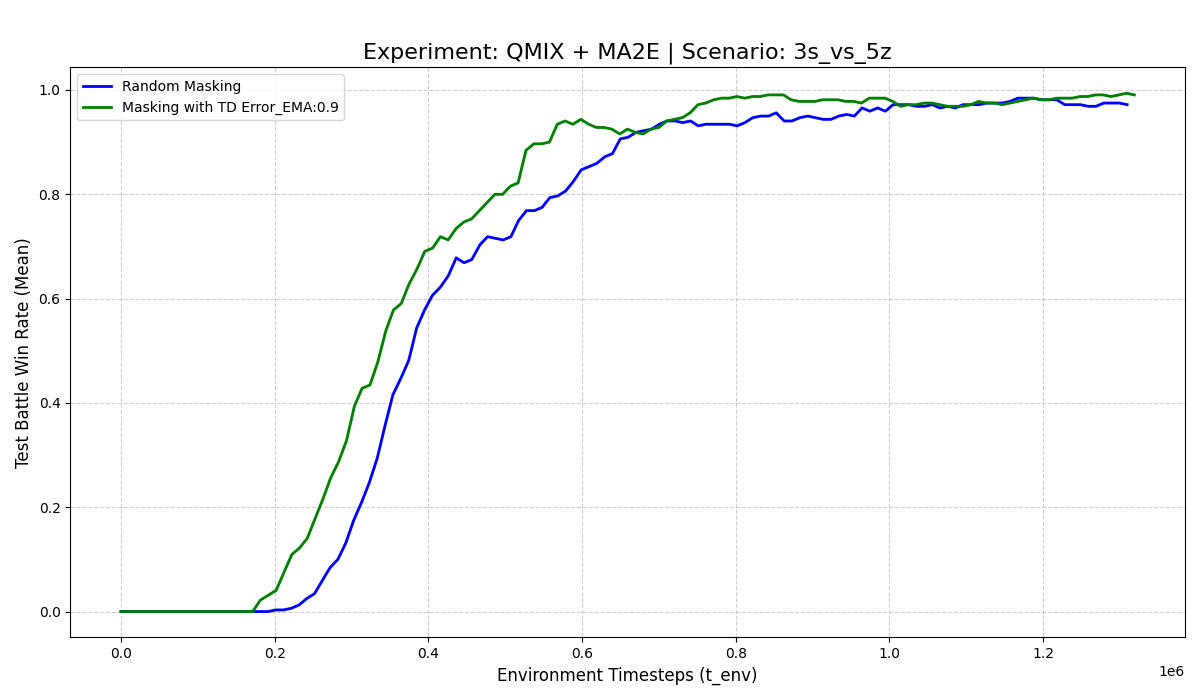
\includegraphics[width=0.5\textwidth]{images_pfe/results_li-ma2e/test_battle_won_mean_3s_vs_5z_ema_0.9_smoothed.png}}%
\hfill%
\subfloat[\label{fig:ema_0.1} EMA with ($\alpha=0.1$)]{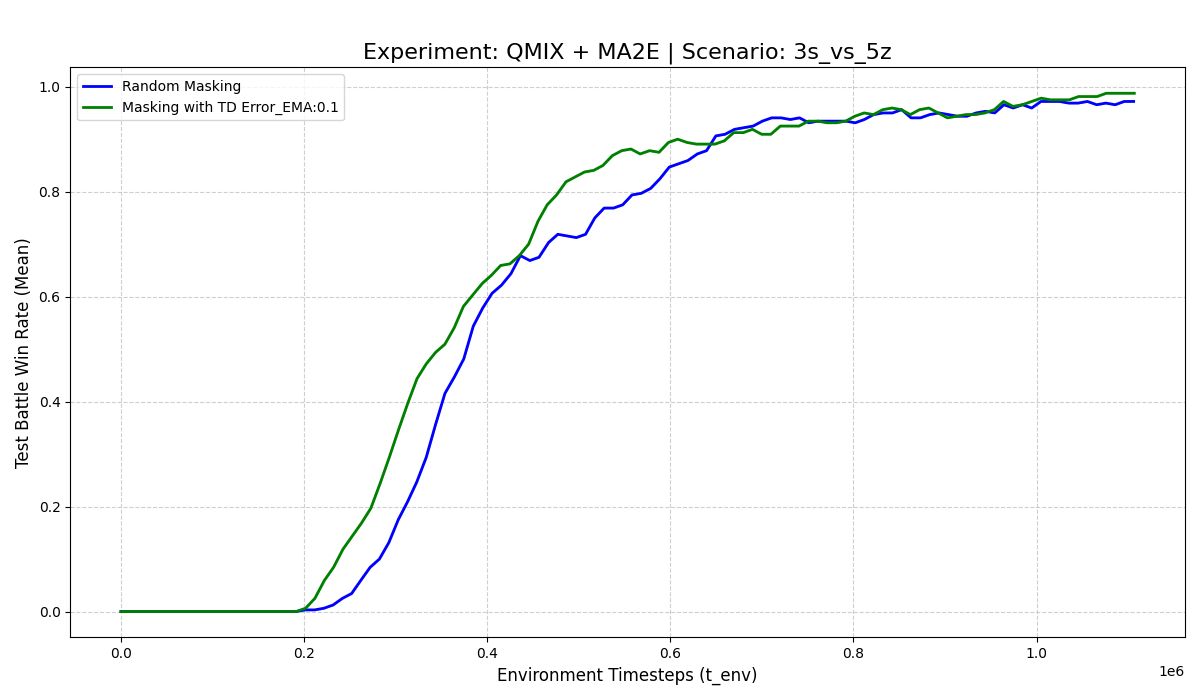
\includegraphics[width=0.5\textwidth]{images_pfe/results_li-ma2e/test_battle_won_mean_3s_vs_5z_ema_0.1_smoothed.png}}%
\caption{Performance comparison of EMA-based masking strategies with different decay rates $\alpha$ against the baseline Random Masking on the \texttt{3s\_vs\_5z} SMAC map. The plots show the mean test win rate over environment timesteps.}
\label{fig:ema_comparison}
\end{figure}
The performance of the EMA strategy with a decay rate of $\alpha=0.9$ was compared against the baseline Random Masking, with the results for the \texttt{3s\_vs\_5z} scenario presented in Figure~\ref{fig:ema_comparison}.
The results clearly demonstrate that our EMA-based masking (green line) achieves significantly better sample efficiency than the baseline (blue line). The $LI-{MA}^2E$ framework learns the task much faster, reaching a high win rate at approximately 0.6 million timesteps, while the baseline requires around 0.8 million timesteps to achieve similar performance. While both methods eventually converge to a near-perfect win rate on this map, the accelerated learning curve of the EMA method confirms our hypothesis that intelligently guiding the masking process is more effective than a random strategy.

Despite this improved efficiency, the limitation of this global EMA approach is its inherent inertia. An agent that has recently improved its policy might still be masked due to its poor history, potentially slowing down optimal convergence. This observation motivated the development of our next method, which analyzes performance dynamics on a more granular, intra-episode level.


\subsection{Method 2: Variance-Directional-Drop Score (VDS)}
\label{subsec:vds_method}

Our second approach analyzes the dynamics of an agent's TD-error within a single episode. The VDS was designed to identify which agents are \textit{learning}, which are \textit{forgetting}, and how turbulent their learning process is. The hypothesis is that the best candidates for masking are agents whose performance is not only getting worse but is also highly unstable.

\paragraph{Implementation Details}
The VDS score is a product of two factors: a Variance Factor that measures turbulence and a Directional-Drop Factor that measures the learning trend. The formula is defined as:
\begin{equation}
    \text{VDS} = \left(\frac{\sigma^2}{\sigma^2 + 1}\right) \times \left(\frac{e_0 - e_T}{|e_0| + \epsilon}\right)
\label{eq:vds}
\end{equation}

\begin{itemize}
\item \textbf{$\left(\frac{\sigma^2}{\sigma^2 + 1}\right)$ : } This term quantifies the \textit{turbulence} or volatility of an agent's TD-error curve throughout the episode. A value close to 1 signifies a \textit{bumpy} learning process with significant oscillations and spikes, while a value close to 0 indicates a smooth and calm learning curve. This factor rewards episodes that are eventful.
\item \textbf{$\left(\frac{e_0 - e_T}{|e_0| + \epsilon}\right)$} This term determines the overall trend of the error from the start of the episode. A positive result signifies that the agent is \textit{learning}, as its prediction error has dropped. Conversely, a negative result signifies that the agent is \textit{forgetting,} as its error has increased over the course of the episode.
\end{itemize}

By multiplying these factors, the sign of the resulting VDS score indicates whether an agent is a learner (+) or a forgetter (−), while the magnitude reflects the drama of the change. Our masking strategy prioritizes agents identified as \textit{chaotic forgetters}: those who exhibit both high variance and a negative directional drop. These agents yield a large negative VDS score and are masked first, forcing the MAE to focus its representational power on the most unstable and deteriorating policies.

\paragraph{Results and Limitations}

\begin{figure}[h]
    \centering
    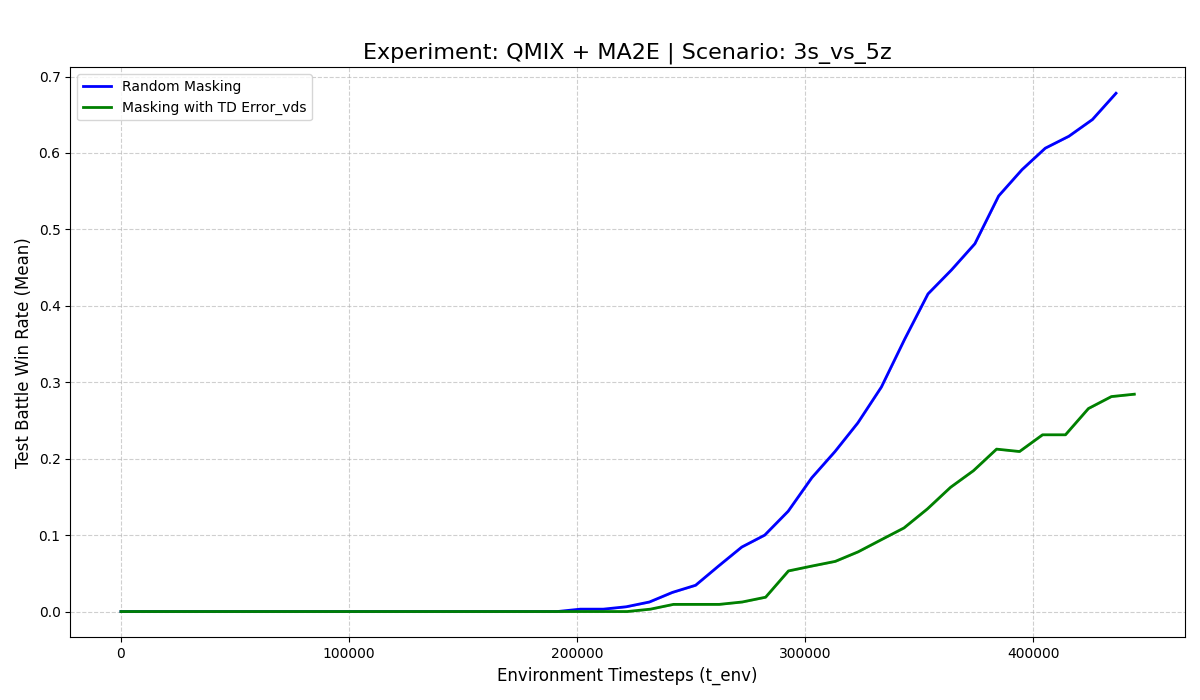
\includegraphics[width=0.8\textwidth]{images_pfe/results_li-ma2e/test_battle_won_mean_3s_vs_5z_vds_smoothed.png}
    \caption{Performance comparison of the VDS masking strategy against the baseline Random Masking on the \texttt{3s\_vs\_5z} SMAC map. The plot shows the mean test win rate over environment timesteps.}
    \label{fig:vds_vs_random}
\end{figure}

The performance of the VDS masking strategy was compared against the baseline Random Masking, with the results for the \texttt{3s\_vs\_5z} scenario presented in Figure~\ref{fig:vds_vs_random}.

Contrary to our initial hypothesis, the results show that the VDS masking strategy (green line) significantly underperforms compared to the baseline Random Masking (blue line). Throughout the training process, the win rate for the VDS-guided agent remains considerably lower than that of the agent using a random strategy. By the end of the depicted training run at approximately 450,000 timesteps, the baseline achieves a win rate of nearly 70\%, while the VDS method struggles to surpass 30\%.

Given the clear negative performance trend and the computational time required, the experiment for the VDS method was halted early, as it was evident that further training was unlikely to yield a competitive result.

This poor performance likely stems from the core limitations of the VDS metric. By relying on the start and end points of an entire episode, VDS may generate a noisy or misleading signal. For instance, an episode with high variance in the TD-error could result in a high-magnitude VDS score, causing a potentially effective agent to be masked frequently. As discussed, the directional-drop component also fails to distinguish between an agent that is truly \textit{forgetting } and one that is simply encountering a difficult, new part of the state space. The combination of these factors appears to create a disruptive, rather than helpful, curriculum for the MAE module, ultimately hindering the overall learning process. This result underscores the difficulty of designing a robust masking heuristic and strongly motivates the development of a more reliable score, REFDS, which focuses on recent-step dynamics.
A key limitation of \texttt{VDS} lies in its interpretation of an increasing TD-error trend as definitive \textit{forgetting}. While an agent's error increasing over an episode can be a signal of forgetting, this is not always the case. The rising TD-error could mean one of two distinct things:

\begin{enumerate}
    \item \textbf{Forgetting or Poor Generalization:} If an agent has seen the early parts of an episode's trajectory more often during training, it will predict those values well, leading to a low TD-error. If the error then rises in the later, less-frequently seen states, it suggests the agent may have \textit{forgotten} how to behave there or has failed to generalize its knowledge from the familiar states. This is a plausible sign of forgetting.
    
    \item \textbf{Encountering Under-Trained States:} If the later states in the trajectory are simply underrepresented in the replay buffer, a high TD-error is not a sign of forgetting, but rather an indication that the agent is still actively learning about this unfamiliar part of the state space.
\end{enumerate}
However, its reliance on the start and end points of an entire episode can sometimes be misleading. For example, an agent might improve significantly for most of the episode but then start to \textit{forget} right at the end; VDS might still classify this as overall \textit{learning} and fail to mask the agent when it needs it most. This limitation motivated the development of a score that focuses specifically on the most recent timesteps.


\subsection{Method 3: Recent Error and Forgetting Detection (REFDS)}
\label{subsec:REFDS_method}

To overcome the full-episode focus of VDS and its inability to capture short-term dynamics, we developed REFDS. This score is designed to identify agents that are problematic \textit{right now} by analyzing only the most recent timesteps of their experience. The hypothesis is that a more accurate and timely signal can be derived by considering two factors from an agent's recent history: its current average error level and any immediate evidence of \textit{forgetting} (a rising error trend).


\paragraph{Implementation Details}

The \texttt{REFDS} score is computed per-agent using only the most recent batch of TD-errors, focusing on the last 25\% of each trajectory \\ ($k = \lfloor \text{trajectory\_length} / 4 \rfloor$) to capture recent performance trends. It combines the mean TD-error (magnitude of recent errors) and the slope of TD-errors (directional trend, penalizing worsening performance).
The score is calculated as:
\begin{equation}
    \text{REFDS} = 0.6 \cdot \overline{|\text{TD}|}_k + 0.4 \cdot \text{ReLU}(\text{slope}_k)
    \label{eq:REFDS}
\end{equation}

where $\overline{|\text{TD}|}_k$ is the mean of absolute TD-errors over the last $k$ steps, and $\text{slope}_k$ is the trend over that same window.

\paragraph{Key Properties}
\begin{itemize}
    \item \textbf{Timestep-Local:} Uses only the latest batch of experience, requiring no historical data buffer.
    \item \textbf{Adaptive:} The score naturally targets agents with either large-magnitude errors or a worsening error trend, focusing learning where it is most needed.
\end{itemize}


This approach ensures that fine-tuning prioritizes agents with immediate, high-impact errors while remaining computationally lightweight. The weights (0.6, 0.4) and the window size $k$ are tunable hyperparameters that balance the sensitivity between error magnitude and trend severity.



\paragraph{The purpose of the ReLU function in the REFDS Formula: }
The purpose of the ReLU function is to isolate and penalize only the agents that are actively \textit{forgetting}, without penalizing agents that are actively learning.
Here's the breakdown of the logic:
\begin{itemize}
    \item \textbf{The $\text{slope}_k$ term, $(\text{TD}_{\text{end}} – \text{TD}_{\text{mid}}) / k$}, calculates the recent trend of the TD-error.
   \item By applying $\text{ReLU}(\text{slope}_k)$, we transform the slope value:
\begin{itemize}
    \item If the slope is positive (forgetting), ReLU passes the value through, adding a penalty to the \texttt{REFDS} score.
    \item If the slope is negative (learning), ReLU outputs zero. This is crucial because it ensures that agents who are learning effectively are not \textit{penalized twice} for having a steep (but beneficial) drop in their error.
\end{itemize}
    % \item A positive slope indicates that the error is increasing, which is our signal for \textit{forgetting}.
    % \item A negative slope indicates that the error is decreasing, which is a sign of successful learning.
\end{itemize}
% By applying $\text{ReLU}(\text{slope}_k)$, we transform the slope value:
% \begin{itemize}
%     \item If the slope is positive (forgetting), ReLU passes the value through, adding a penalty to the \texttt{REFDS} score.
%     \item If the slope is negative (learning), ReLU outputs zero. This is crucial because it ensures that agents who are learning effectively are not \textit{penalized twice} for having a steep (but beneficial) drop in their error.
% \end{itemize}
The ReLU acts as a filter, allowing the formula to focus exclusively on the undesirable behavior of an upward drift in error, making the \textit{Forget-Penalty} term more precise.
\paragraph{Results and Limitations}
\begin{figure}[h]
    \centering
   
        
    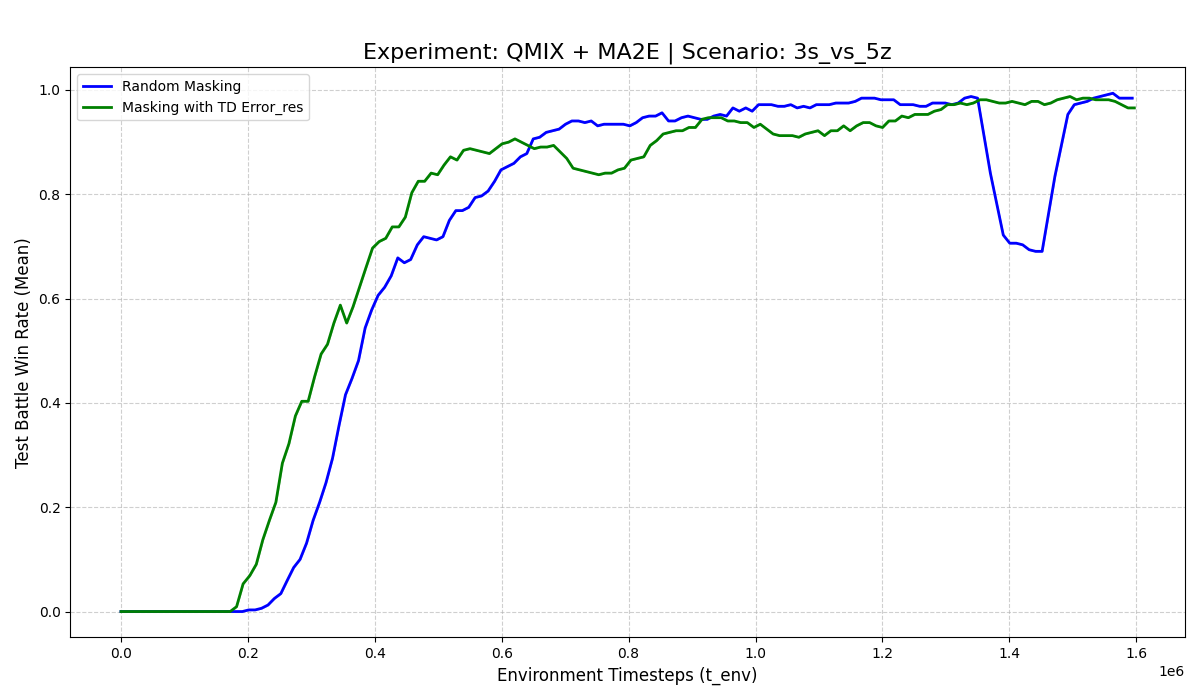
\includegraphics[width= 0.9\linewidth]{images_pfe/results_li-ma2e/test_battle_won_mean_3s_vs_5z_res_smoothed_full.png}
 
  
    \caption{Performance comparison of the REFDS masking strategy against the baseline Random Masking on the \texttt{3s\_vs\_5z} SMAC map. The plot shows the mean test win rate over environment timesteps.
    }
    \label{fig:REFDS_vs_random}
\end{figure}

The performance of the REFDS masking strategy was compared against the baseline Random Masking on the \texttt{3s\_vs\_5z} scenario, with the results presented in Figure~\ref{fig: REFDS_vs_random}.

The results clearly demonstrate that the REFDS strategy (green line) provides a significant improvement in sample efficiency over the baseline (blue line). The REFDS method begins learning notably earlier and maintains a consistent performance lead throughout the critical training phase between approximately 0.2 million and 0.8 million timesteps.

While the Random Masking baseline eventually catches up and both methods are capable of solving this map by reaching a near-perfect win rate, the accelerated learning curve of REFDS is substantial. This confirms that a focused masking strategy based on recent learning dynamics is highly effective at speeding up the training process compared to an uninformed, random approach.

\texttt{REFDS} introduces its own set of challenges and limitations:
\begin{itemize}
    \item \textbf{Computational Overhead:} Compared to the simpler EMA or VDS scores, calculating \texttt{REFDS} for every agent at every episode is more computationally intensive, as it requires storing and processing a sliding window of recent TD-errors.
    
    \item \textbf{Hyperparameter Sensitivity:} The performance of \texttt{REFDS} is dependent on the careful tuning of its key hyperparameters.
    \begin{itemize}
        \item \textit{Window Size ($k$):} The choice of the look-back window is a trade-off. A shorter window reacts faster but can be noisy, while a longer window is smoother but slower to adapt. The optimal value can be scenario-dependent.
        
        \item \textit{Component Weights (0.6 / 0.4):} The weights assigned to the mean-error versus the forgetting-penalty must be balanced. Over-emphasizing one component can cause the score to miss the nuances of the other, requiring careful adjustment to achieve the best results.
    \end{itemize}
\end{itemize}
However, REFDS still operates on the TD-error in isolation. It treats all errors equally, regardless of the context provided by an agent's observation. For example, a high TD-error from an agent seeing very little might be less informative for the MAE to reconstruct than a high TD-error from an agent observing a complex battlefield interaction. This realization prompted our final investigation into a method that contextualizes the error signal with the agent's observation.
\subsection{Method 4: Observation-Weighted TD-Error}

Our final investigation attempted to contextualize an agent's learning error with the \textit{richness} of its observation. The previous methods, including REFDS, treat the TD-error signal in isolation. However, a high TD-error from an agent seeing very little might be less informative for the MAE to reconstruct than a high TD-error from an agent observing a complex battlefield interaction.
The hypothesis for this method is that an agent's failure is most significant if it is failing despite receiving a large amount of information. To quantify the amount of information an agent is \textit{seeing,} we use the L2 norm of its observation vector.

\paragraph{Implementation Details}
The masking score is calculated as a direct product of the agent's performance error and its observation magnitude:
\begin{equation}
    \text{Masking Score} = |\text{TD-error}| \times \| \text{Observation} \|_2
    \label{eq:obs_weighted_td}
\end{equation}
The intuition behind this score can be broken down into four cases:
\begin{itemize}
    \item \textbf{High TD-error \& High L2-norm:} The agent receives a lot of information but still fails to predict correctly. It is likely \textit{confused} or \textit{overwhelmed} and is a prime candidate for masking.
    \item \textbf{High TD-error \& Low L2-norm:} The agent sees very little and is still performing poorly. Its observation is uninformative, making it another good candidate for masking.
    \item \textbf{Low TD-error \& High L2-norm:} The agent sees a lot and learns well. This is a strong, stable agent that should be kept as an anchor for the MAE's reconstruction.
    \item \textbf{Low TD-error \& Low L2-norm:} The agent is stable but has a limited view. This agent is likely harmless and can be kept.
\end{itemize}

\paragraph{Results and Limitations}


\begin{figure}[h]
    \centering
    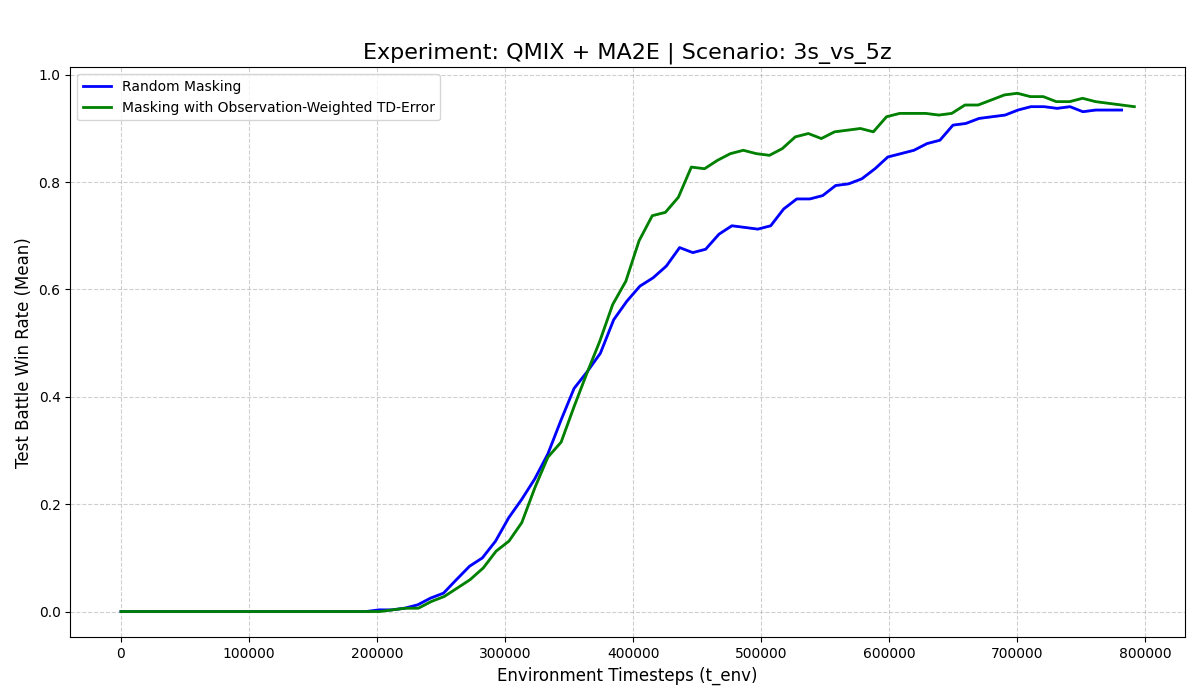
\includegraphics[width=0.8\textwidth]{images_pfe/results_li-ma2e/test_battle_won_mean_3s_vs_5z_Observation-Weighted_TD_smoothed.png}
    \caption{Performance comparison of the Observation-Weighted TD-Error masking strategy against the baseline Random Masking on the \texttt{3s\_vs\_5z} SMAC map. The plot shows the mean test win rate over environment timesteps.}
    \label{fig:obs_weighted_vs_random}
\end{figure}

The performance of the Observation-Weighted TD-Error strategy was compared against the Random Masking baseline on the \texttt{3s\_vs\_5z} map, with results shown in Figure~\ref{fig:obs_weighted_vs_random}.

The results present a nuanced picture. Unlike some previously tested methods, this strategy does not show a significant improvement in sample efficiency during the initial learning phase. The performance of the observation-weighted method (green line) closely tracks that of the random baseline (blue line) for the first approximately 450,000 timesteps.

However, in the later stages of training, a clear advantage emerges. The Observation-Weighted TD-Error strategy begins to outperform the baseline, converging to a high win rate more quickly and smoothly. This delayed improvement supports our analysis of the method's limitations; the L2 norm of the observation is not always a reliable or stable proxy for the usefulness of the information an agent receives. The initial phase, where it performs similarly to random masking, suggests that this heuristic may introduce noise that counteracts the benefit of the TD-error signal early in training. Only once the underlying value functions become more stable does the contextual information from the observation norm appear to provide a consistent, beneficial signal.

\subsection{Method 5: Adaptive Masking with Mean TD-Error Thresholding}

After investigating complex heuristics like VDS and observation-weighting, our final approach returns to the most direct signal of agent performance: the TD-error itself. The previous methods, while insightful, introduced additional complexity and sensitive hyperparameters. The hypothesis for this final method is that a simple, direct, and adaptive threshold is more robust and effective.

Instead of trying to interpret the dynamics of the error (like VDS or REFDS), we simply posit that agents performing worse than the current batch average are the most beneficial candidates for masking. This approach is designed to be adaptive throughout training. Early on, when agent performance varies widely, the mean TD-error provides a natural and dynamic cutoff. Late in training, when all agents perform well and have similar, low TD errors, a fixed threshold would fail. Therefore, a top-$k_1$ fallback mechanism is included to ensure that the MAE continues to be fine-tuned on the relatively weaker agents, even when all agents are strong.

\paragraph{Implementation Details}
It is important to note that this smart masking strategy is only applied during the policy fine-tuning phase. The initial pre-training of the MA$^2$E module is still conducted using random masking to allow the model to learn general, unbiased agent representations.

The fine-tuning process for this method uses only the TD errors generated from the most recent training batch, ensuring minimal overhead. The step-by-step process is as follows:
\begin{enumerate}
    \item \textbf{Compute TD-Error per Agent:} For each agent $a$, the TD-error is calculated as the difference between its predicted Q-value and the target value:
    \begin{equation}
        \label{eq:td_error_simple}
        \text{TD-error}_a = Q_a - \text{Target}_a
    \end{equation}

    \item \textbf{Agent Selection with Adaptive Threshold:} The core of the method lies in its two-stage selection logic:
    \begin{itemize}
        \item First, the mean of the absolute TD-errors is computed across all agents in the current training batch.
        \item Any agent whose individual TD-error is above this batch mean is selected for masking.
        \item As a fallback, if no agent's error exceeds the mean (a situation common late in training), the top-$k$ agents with the highest TD-errors are chosen instead.
    \end{itemize}

    \item \textbf{Apply Masking:} The observation-action history tokens of all selected agents are masked (e.g., zeroed out) before being passed as input to the MAE module for reconstruction.
\end{enumerate}
\paragraph{Results and Limitations}

\begin{figure}[h]
    \centering
    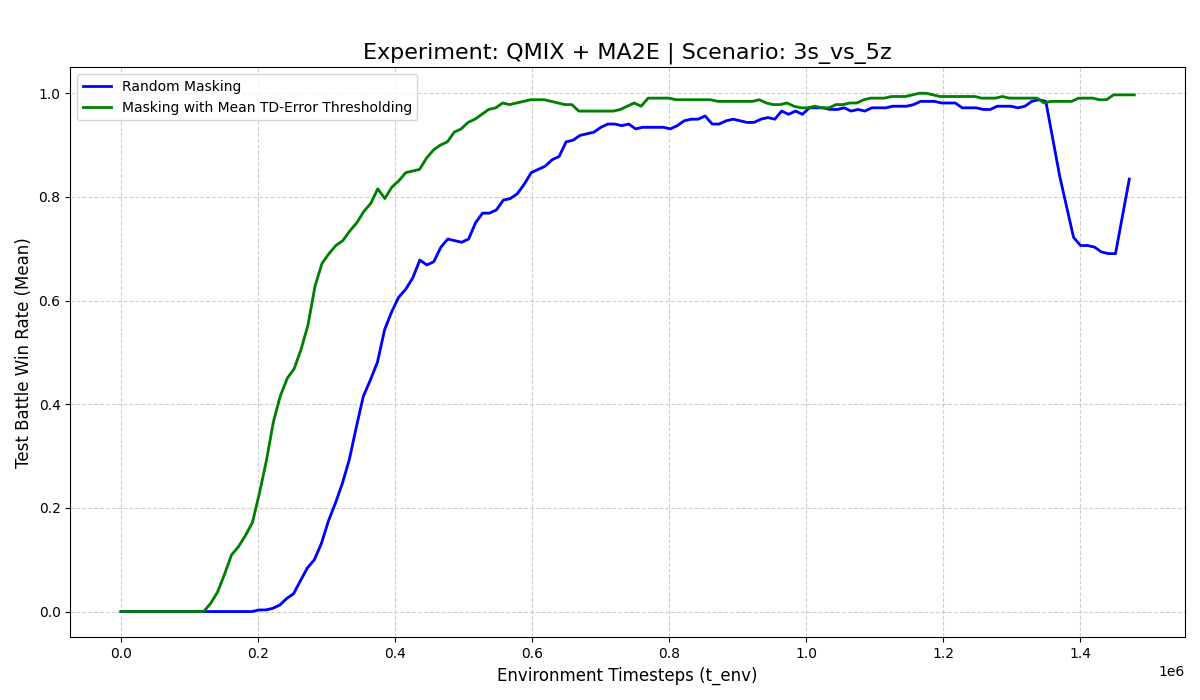
\includegraphics[width=0.8\textwidth]{images_pfe/results_li-ma2e/test_battle_won_mean_3s_vs_5z_Mean_TD-Error_Thresholding _smoothed.png}
    \caption{Performance of the final Adaptive Mean TD-Error Thresholding strategy compared against the Random Masking baseline on the \texttt{3s\_vs\_5z} SMAC map. The plot highlights the superior sample efficiency of the proposed method.}
    \label{fig:mean_td_vs_random}
\end{figure}


Finally, the performance of our proposed Adaptive Masking with Mean TD-Error Thresholding was compared against the baseline Random Masking. The results on the \texttt{3s\_vs\_5z} map are presented in Figure~\ref{fig:mean_td_vs_random}.

The results demonstrate a dramatic improvement in performance and sample efficiency. The Mean TD-Error Thresholding strategy (green line) learns significantly faster than the baseline (blue line), achieving a near-perfect win rate before 0.6 million timesteps, while the baseline requires over 1.2 million timesteps to reach a similar level of performance.

This final experiment provides a clear conclusion to our investigation of scoring methods. After exploring a global historical average (EMA), episode-level dynamics (VDS), and feature-based heuristics (Observation-Weighted TD-error), the results show that a simple, direct, and adaptive threshold based on the batch-average TD-error is the most robust and effective strategy. It avoids the inertia of the EMA, the ambiguity of VDS, and the heuristic instability of the observation-weighted score. Its superior performance validates our final hypothesis that a straightforward comparison of an agent's immediate error to that of its peers provides the cleanest and most potent signal for guiding the MAE's representational learning.

Therefore, based on this comprehensive empirical analysis, the Adaptive Masking with \textbf{Mean TD-Error Thresholding} was selected as the definitive $LI-{MA}^2E$ framework. All subsequent results presented in this thesis will utilize this final, optimized method.
% This new subsection will contain the summary plot and its analysis.
\subsection{Comparison of Masking Strategies:}

To synthesize the findings from our investigation and provide a clear visual summary, Figure~\ref{fig:all_strategies_comparison} presents a direct comparison of all tested masking strategies on the  \texttt{3s\_vs\_5z} scenario.
\begin{figure}[h]
    \centering
    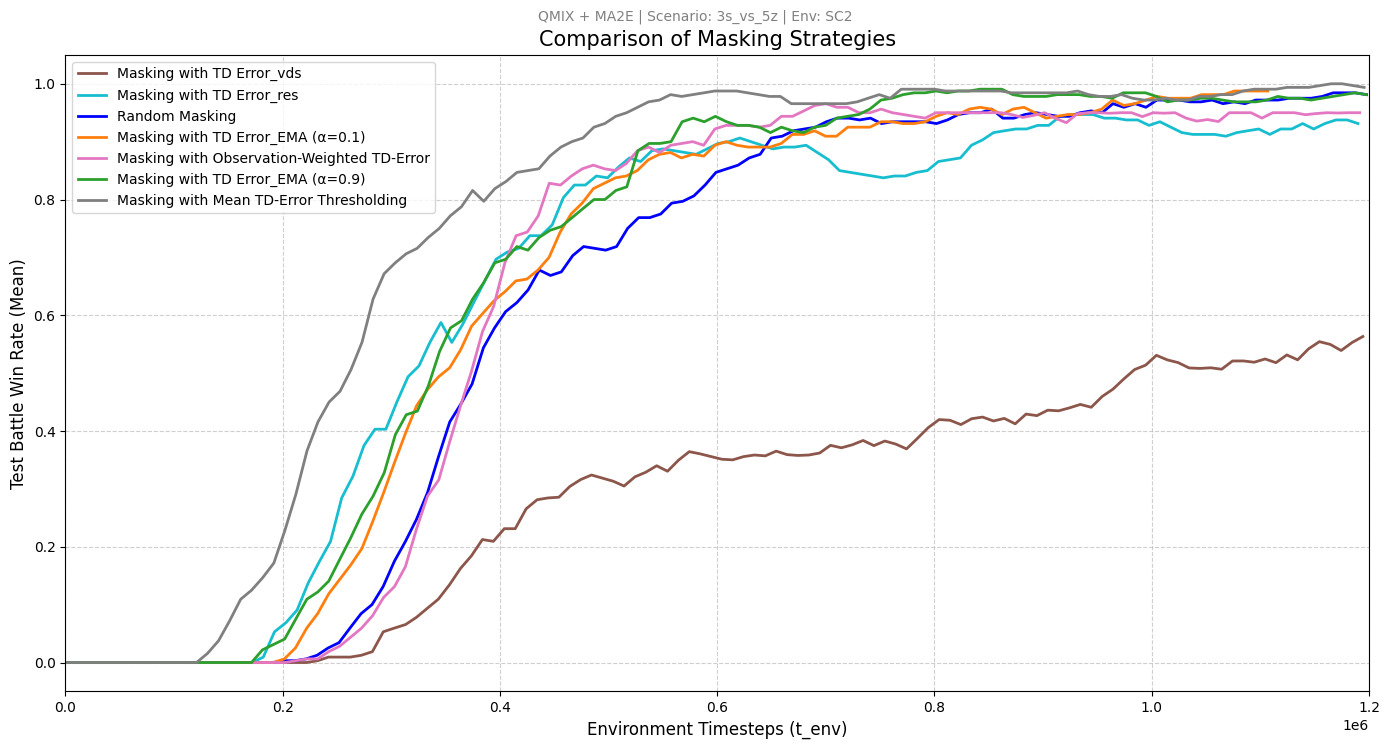
\includegraphics[width=1.0\textwidth]{images_pfe/results_li-ma2e/compare_scores.jpg} 
    \caption{Comprehensive comparison of all evaluated masking strategies on the \texttt{3s\_vs\_5z}  SMAC map. The results visually confirm that the Mean TD-Error Thresholding and REFDS strategies provide the best sample efficiency.}
    \label{fig:all_strategies_comparison}
\end{figure}

The results in Figure~\ref{fig:all_strategies_comparison} provide a clear hierarchy of performance. The \textbf{VDS} strategy significantly hindered learning compared to the random baseline. The \textbf{EMA-based methods} and the \textbf{Observation-Weighted TD-Error} offer marginal improvements over random masking, with the more reactive \textbf{EMA($\alpha=0.9$)} showing the most promise among them.

However, the two most effective strategies are clearly \textbf{REFDS} and our final proposed method, \textbf{Mean TD-Error Thresholding}. Both demonstrate vastly superior sample efficiency, reaching high win rates much earlier than any other approach. This comprehensive result validates our research trajectory, confirming that moving from global averages or flawed episode-level heuristics to reactive, fine-grained signals based on recent TD-error dynamics yields the best performance. While both REFDS and Mean TD-Error Thresholding are highly effective, the latter was chosen as our final framework due to its simpler implementation and more direct, adaptive logic.

% \section{Main Results: Comparative Performance of LI-MA2E}
% \label{sec:main_results}

% Having established the superiority of our Adaptive Mean TD-Error Thresholding strategy in the previous section, we now present a comprehensive performance evaluation of the final LI-MA2E framework. To validate its effectiveness and generalization capabilities, we benchmark our method against the baseline MA2E with random masking across a suite of challenging HARD, MEDIUM, and easy scenarios from the SMAC environment. This section will demonstrate the consistent performance gains achieved by our intelligent masking approach.
% \subsection{Performance on SMAC Scenarios}


% \subsubsection{Scenario: \texttt{3m}}
% Our first evaluation is on the \texttt{3m} scenario, a simple symmetric map that pits \textbf{3 allied Marines against 3 enemy Marines}. Because  \textbf{the agents are homogeneous} and the \textbf{setup is symmetric}, the primary challenge in this map is learning a fundamental cooperative tactic: \textbf{focus-firing}. To win consistently, all three agents must learn to coordinate their attacks on the same enemy target at the same time to eliminate it quickly, rather than spreading their damage ineffectually across multiple targets. This scenario serves as a basic test of coordination. The results are presented in Figure~\ref{fig:3m}.

% \begin{figure}[h]
%     \centering
%     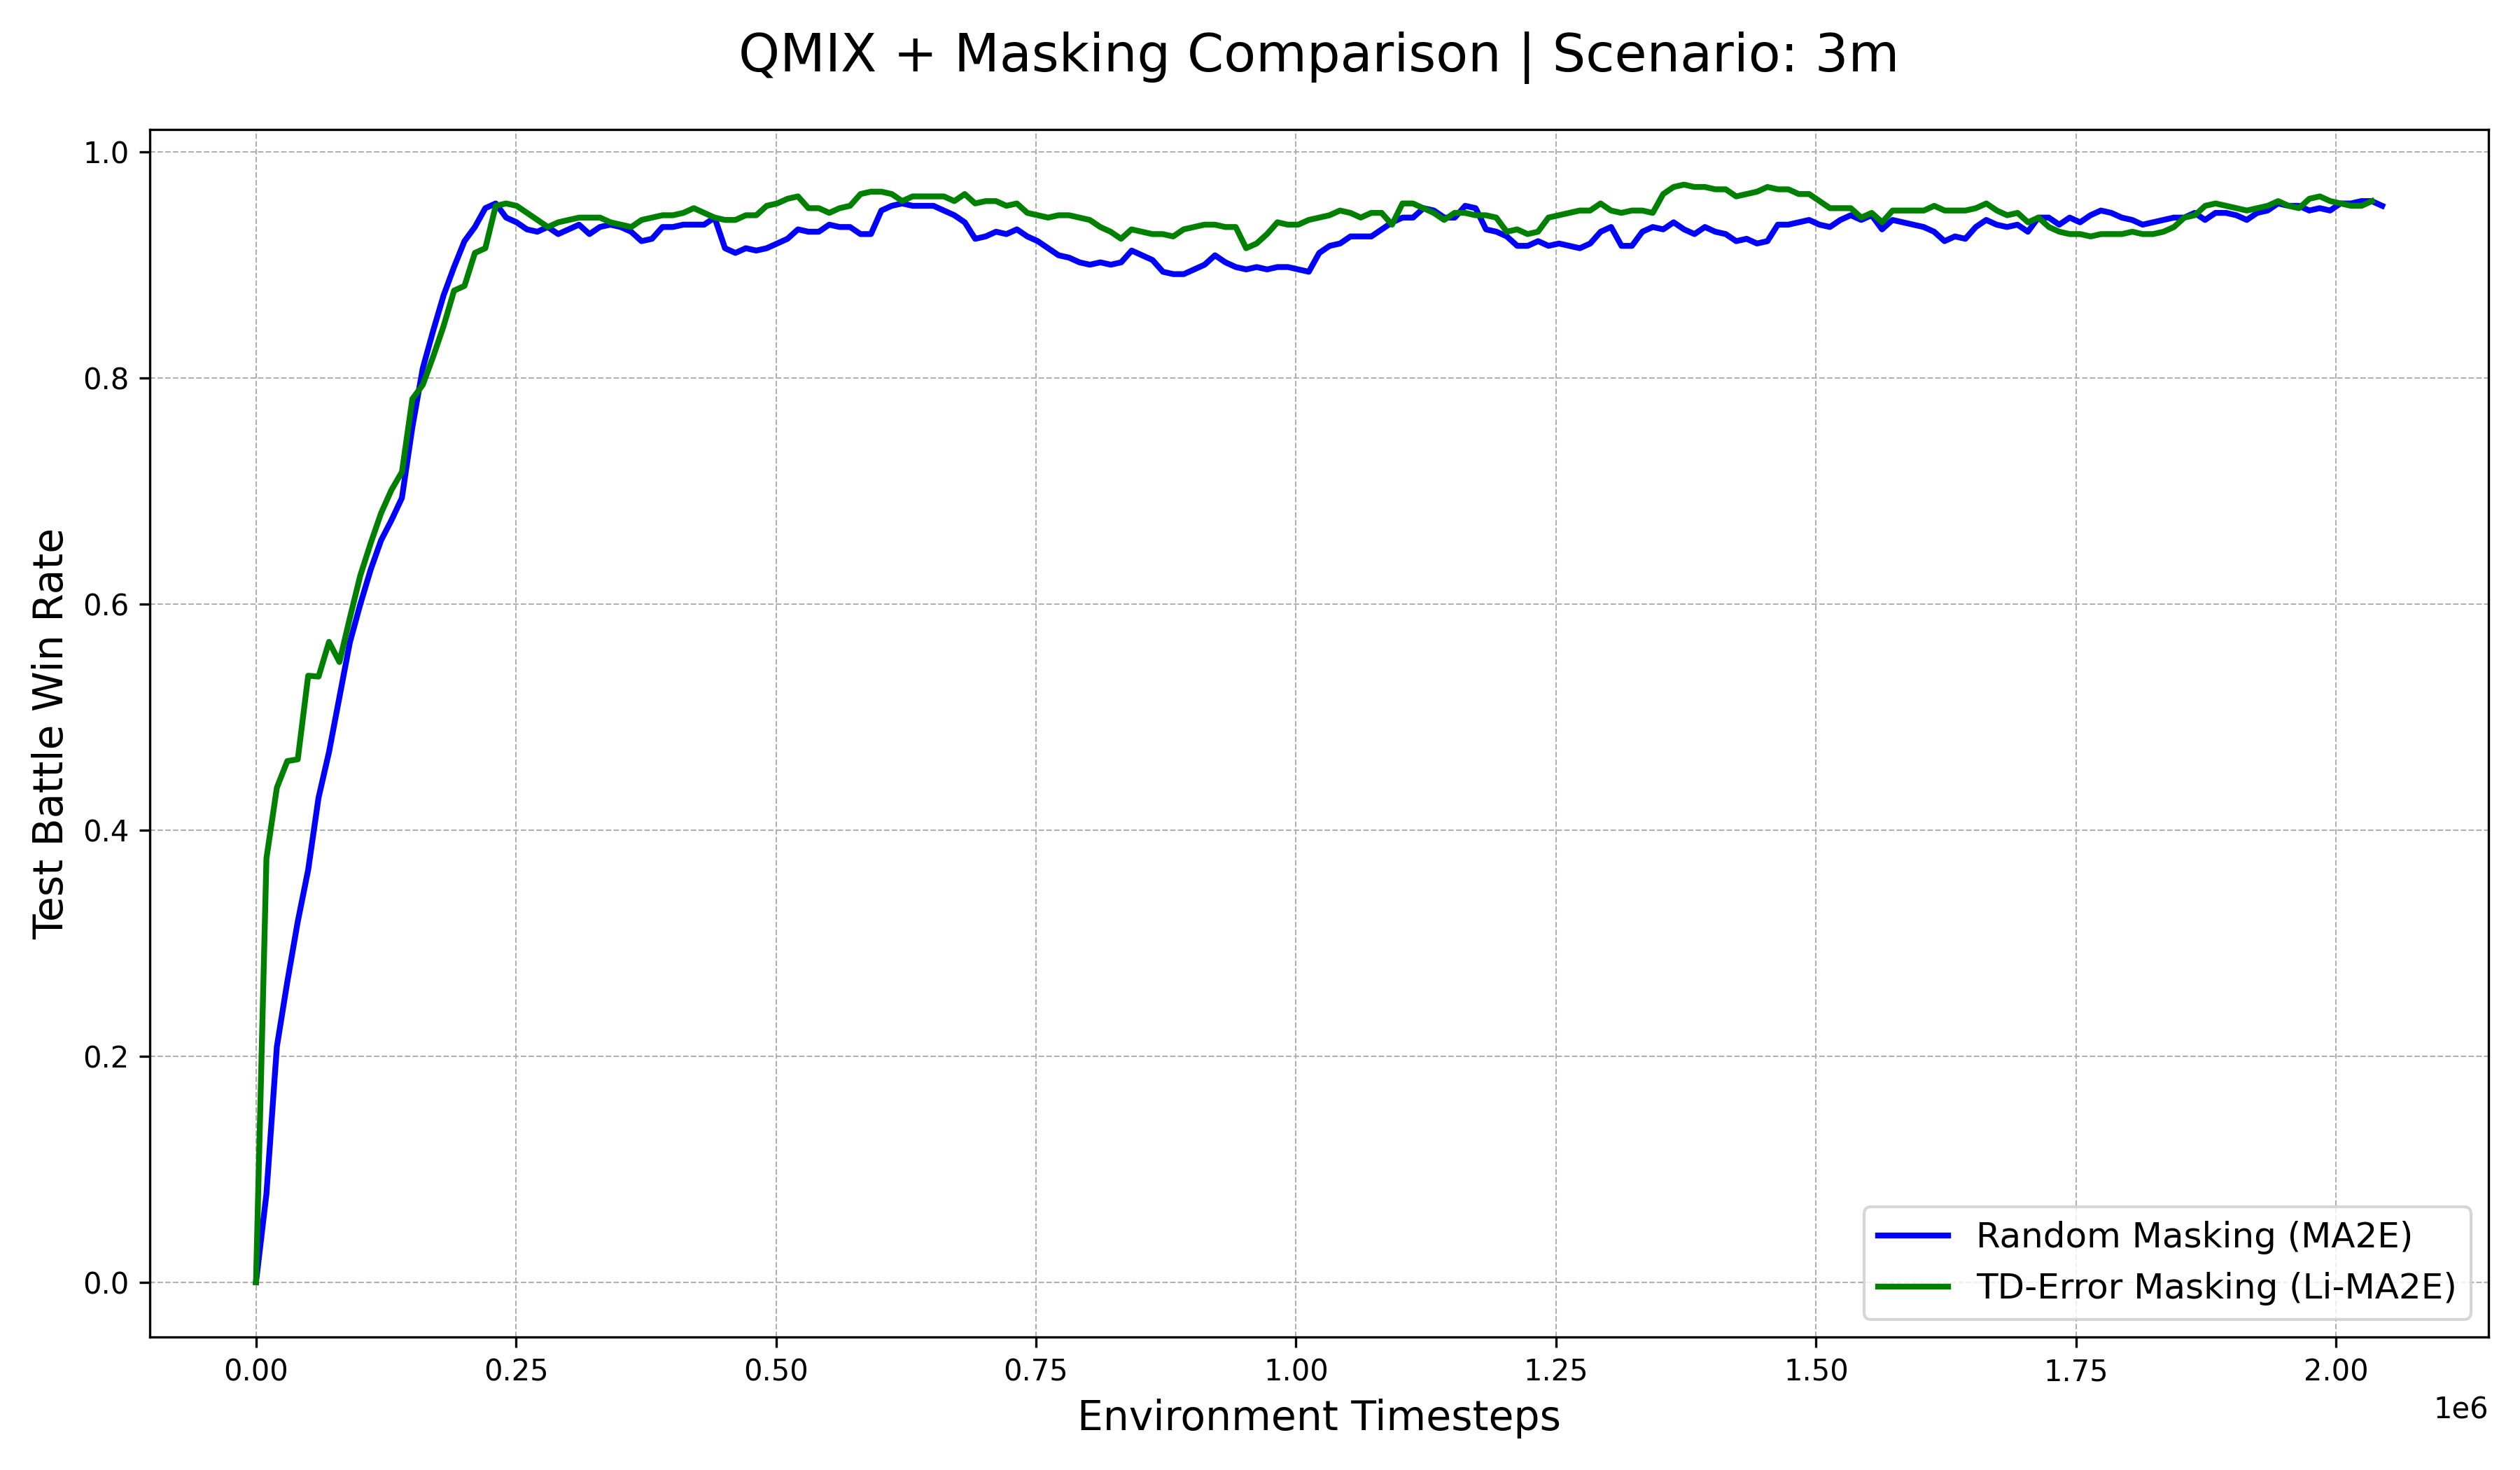
\includegraphics[width=0.8\textwidth]{images_pfe/results_li-ma2e/comparison_plot_3m.png}
%     \caption{Performance comparison on the \texttt{3m} SMAC map. In this simple symmetric scenario, the performance of LI-MA2E is comparable to the random masking baseline.}
%     \label{fig:3m}
% \end{figure}

% \paragraph{Analysis}
% As the learning curves in Figure~\ref{fig:3m} show, the performance of our LI-MA2E framework (green line) is largely comparable to that of the baseline MA2E with random masking (blue line). Both methods learn the task very rapidly, achieving a near-perfect win rate in under 250,000 environment timesteps. Throughout the remainder of the training, both policies maintain a similar high level of performance.

% This result suggests that in simpler scenarios where the need for complex coordination to overcome partial observability is low, the additional guidance provided by our intelligent masking strategy does not yield a significant advantage. The baseline random masking is sufficient for the MAE module to learn the necessary representations to solve this task effectively. This provides an important baseline, demonstrating that our method's complexity does not hinder performance on easy tasks while setting the stage for evaluation on more demanding scenarios.

% \subsubsection{Scenario: \texttt{3s\_vs\_3z}}
% Next, we look at the \texttt{3s\_vs\_3z} scenario. In this test, our \textbf{3 agents control Stalker units}, which can attack from a distance. They face \textbf{3 enemy Zealot units}, which are severe but can only attack up close.

% Because our agents can shoot from far away, the most important skill they must learn is called \textbf{kiting}. Kiting means the Stalkers must keep moving away from the chasing Zealots, while stopping briefly to shoot at them. The goal is to damage the enemy without letting them get close enough to hit back. To do this well, all three of our agents need to work together as a team. The results of this test are shown in Figure~\ref{fig:3s_vs_3z}.

% \begin{figure}[h]
%     \centering
%     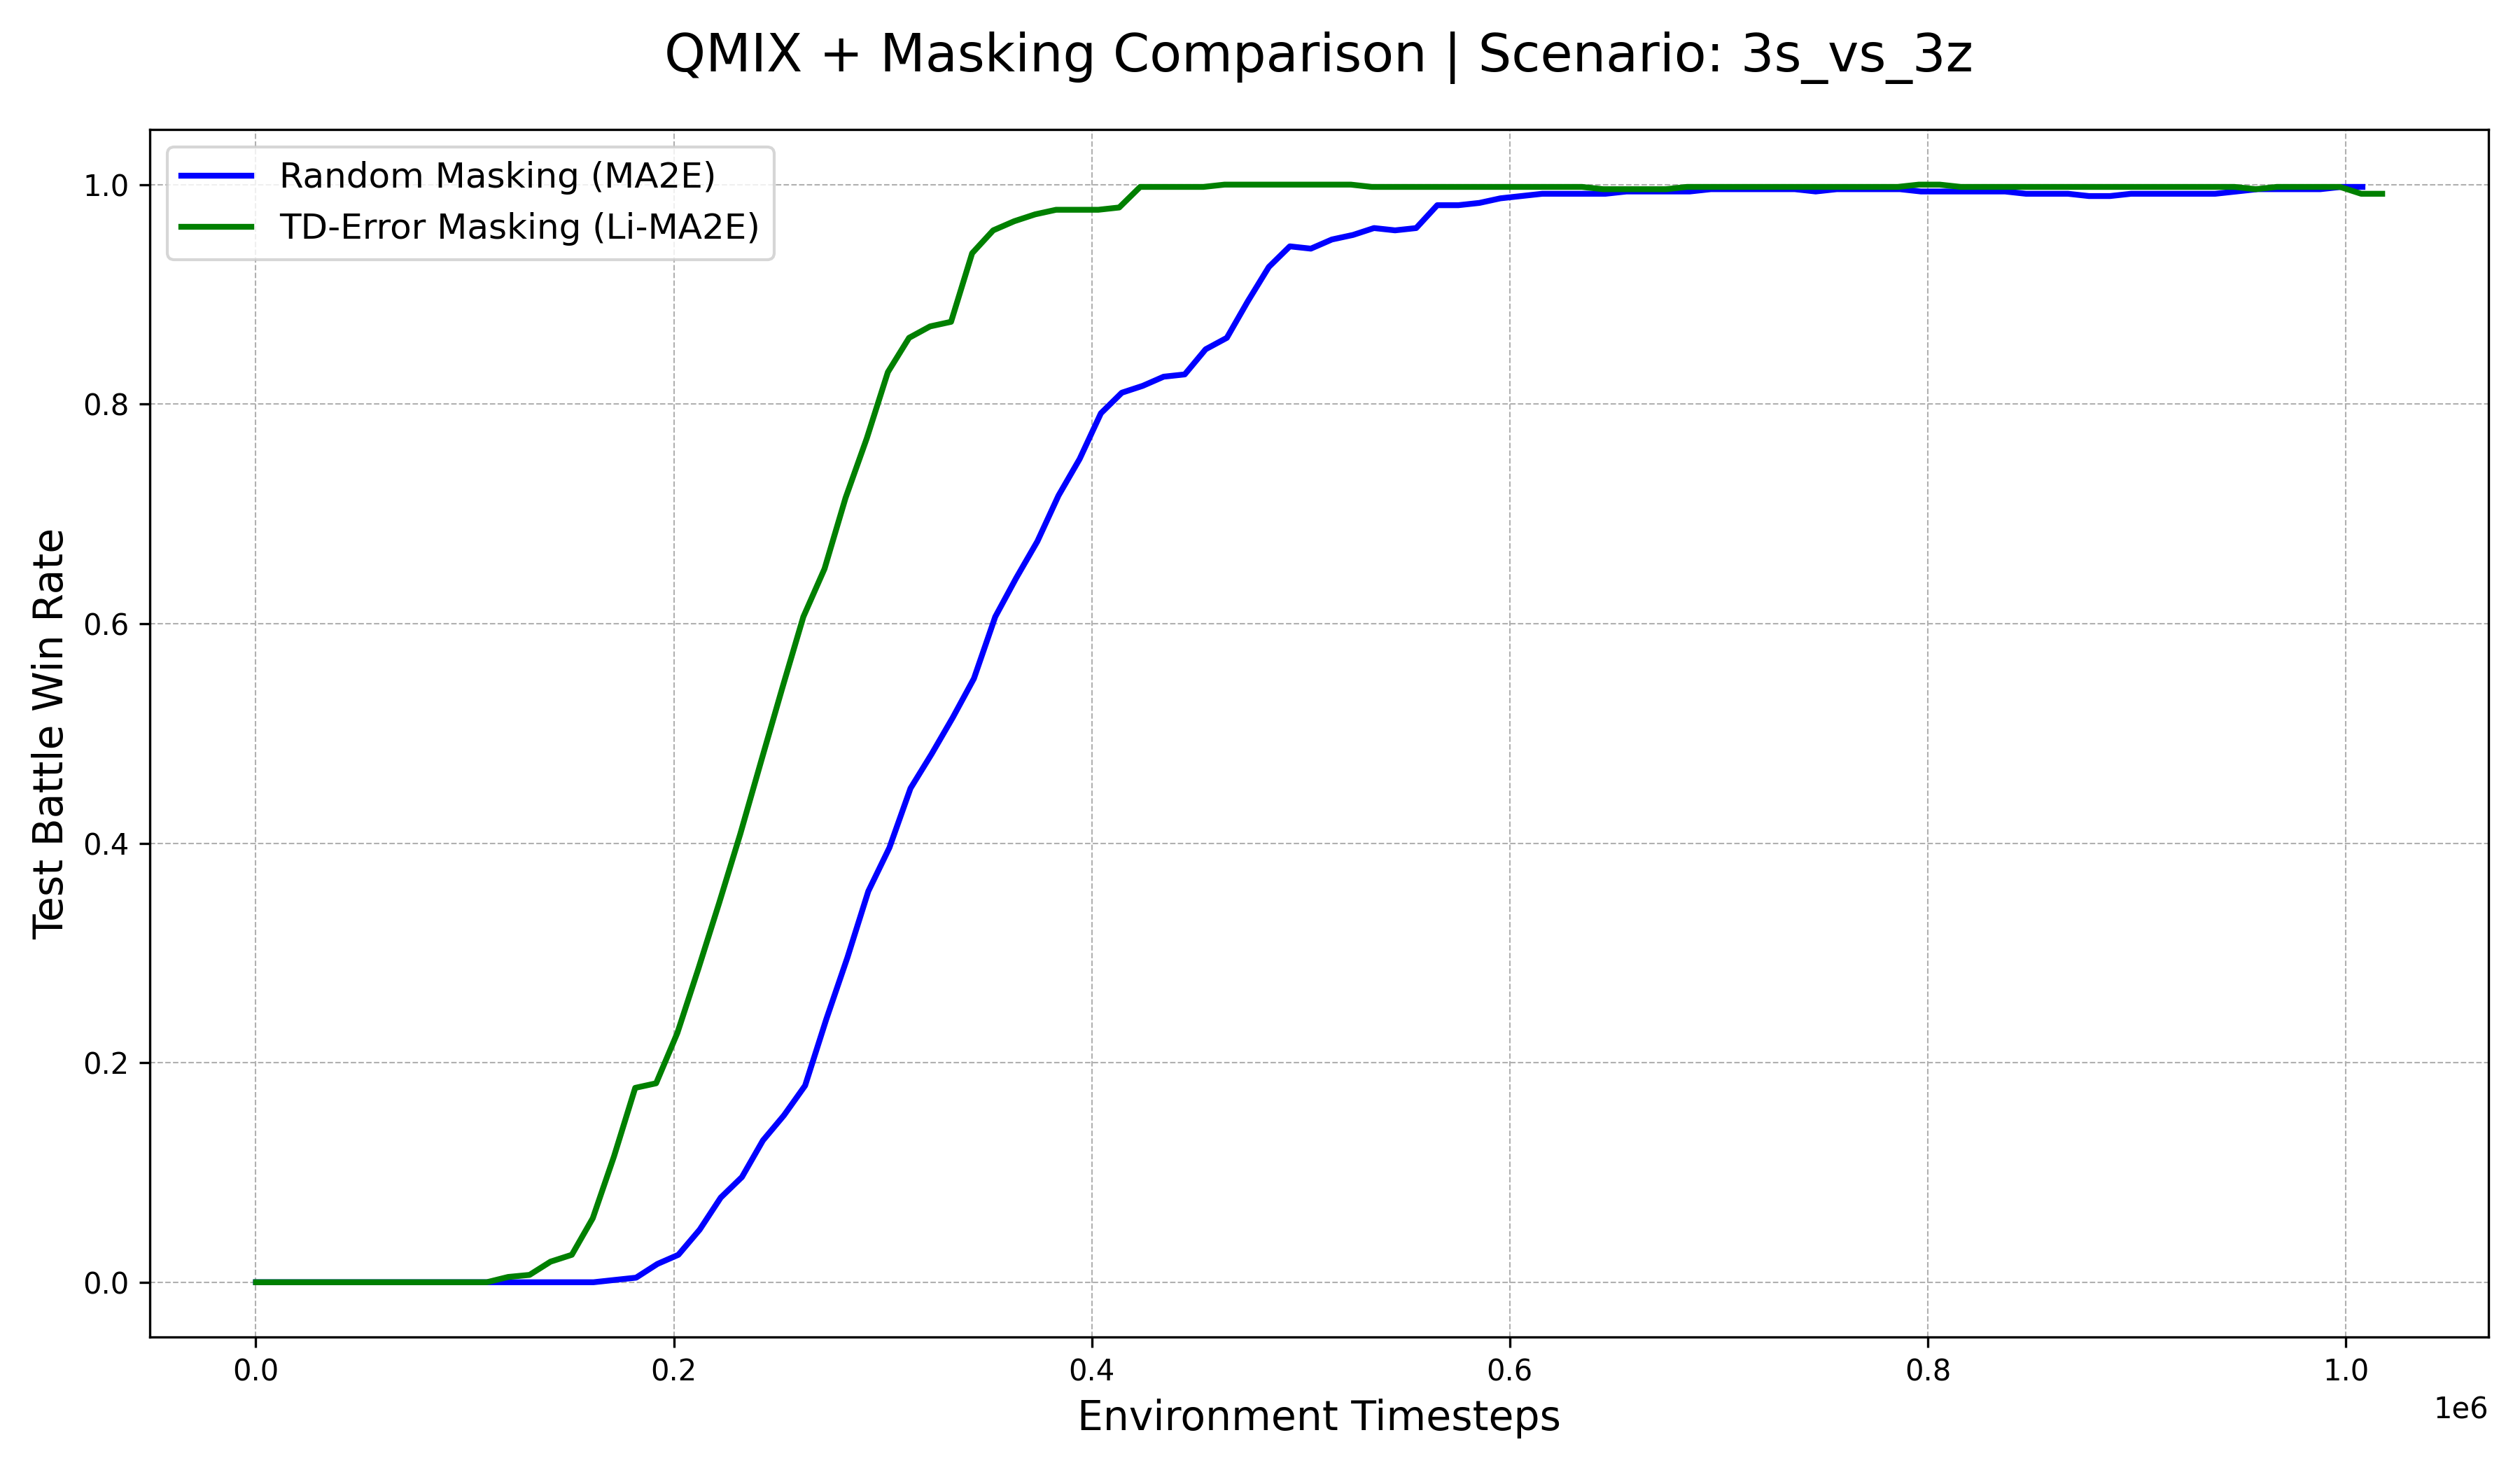
\includegraphics[width=0.8\textwidth]{images_pfe/results_li-ma2e/comparison_plot_3s_vs_3z.png}
%     \caption{Performance comparison on the \texttt{3s\_vs\_3z} SMAC map. LI-MA2E demonstrates significantly improved sample efficiency over the baseline.}
%     \label{fig:3s_vs_3z}
% \end{figure}

% \paragraph{Analysis}
% In the \texttt{3s\_vs\_3z} scenario, the benefit of our LI-MA2E framework becomes immediately apparent. As shown in Figure~\ref{fig:3s_vs_3z}, the agent guided by TD-Error Masking (green line) learns significantly faster than the baseline agent using Random Masking (blue line).

% Our method begins to achieve a non-zero win rate earlier, and its learning curve is considerably steeper, indicating superior sample efficiency. The LI-MA2E agent reaches a perfect win rate at approximately 400,000 timesteps, while the baseline requires around 600,000 timesteps to achieve the same level of performance. This result supports our hypothesis that as scenario complexity increases, an intelligent masking strategy that focuses the MAE's representational power on poorly performing agents provides a distinct advantage, enabling the system to solve the coordination task more rapidly.
% \subsubsection{Scenario: \texttt{3s\_vs\_4z}}

% Now, we test a harder scenario called \texttt{3s\_vs\_4z}. Here, our \textbf{3 Stalker agents}, who can shoot from a distance, must fight against \textbf{4 enemy Zealot units}, which are durable but can only attack up close.

% This test is much more difficult because our agents are \textbf{outnumbered}. To win, they must use two skills together perfectly:
% \begin{enumerate}
%     \item \textbf{Kiting:} They must keep running away from the Zealots to stay safe, while stopping to shoot them.
%     \item \textbf{Focus-Firing:} All three Stalkers must attack the \textit{same} Zealot at the same time to defeat it as quickly as possible.
% \end{enumerate}
% This requires excellent teamwork to succeed. The results of this difficult test are shown in Figure~\ref{fig:3s_vs_4z}.

% \begin{figure}[h]
%     \centering
%      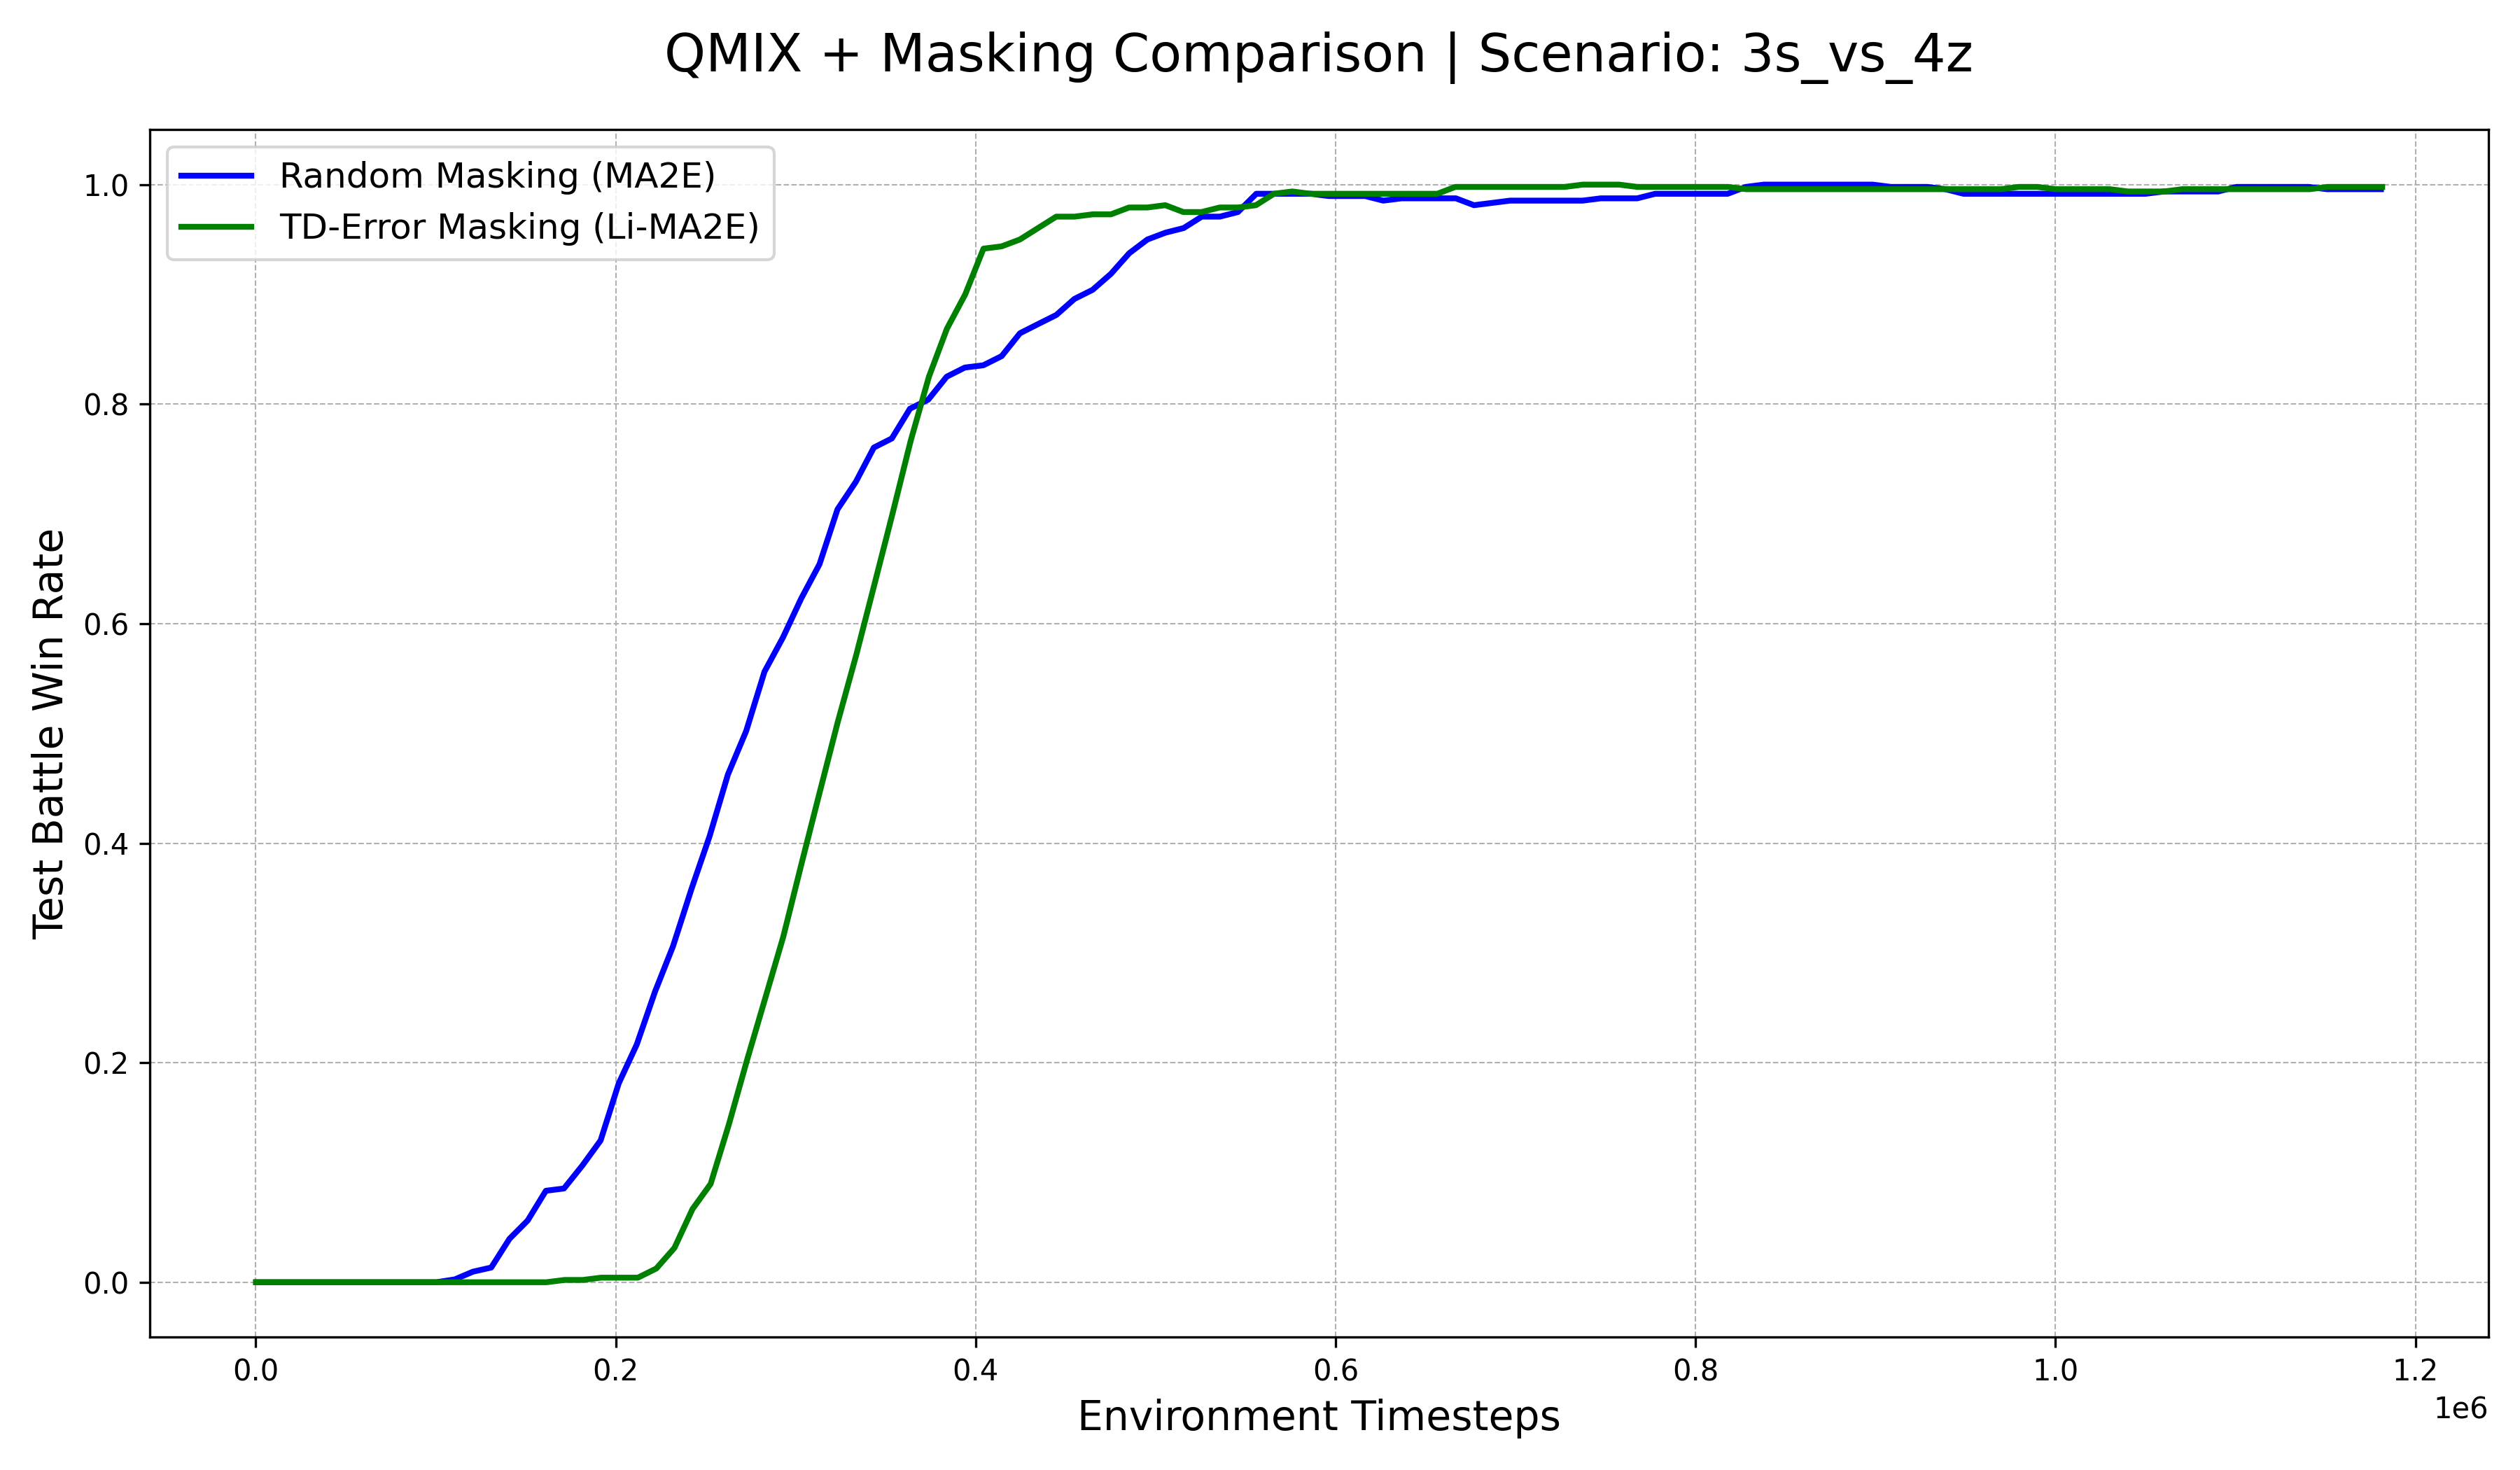
\includegraphics[width=0.8\textwidth]{images_pfe/results_li-ma2e/comparison_plot_3s_vs_4z.png}
%     \caption{Performance comparison on the \texttt{3s\_vs\_4z} SMAC map. The plot shows a trade-off between the faster initial learning of the baseline and the more stable final convergence of LI-MA2E.}
%     \label{fig:3s_vs_4z}
% \end{figure}

% \paragraph{Analysis}
% The \texttt{3s\_vs\_4z} scenario reveals an interesting trade-off between learning speed and final policy stability. As shown in Figure~\ref{fig:3s_vs_4z}, the baseline MA2E with Random Masking (blue line) exhibits a faster initial learning curve, reaching a high win rate more quickly.

% However, a closer look at the convergence phase (after 0.6 million timesteps) shows that our LI-MA2E framework (green line) achieves a more stable and decisive convergence at a 100\% win rate. The baseline's performance, in contrast, shows more fluctuation before finally settling. This suggests that while the exploratory nature of random masking may find a working solution faster in this specific scenario, the guided approach of LI-MA2E produces a more robust and stable final policy.


% \subsubsection{Scenario: \texttt{3s\_vs\_5z}}

% Next, we test our method on \texttt{3s\_vs\_5z}, a very hard challenge from the \texttt{HARD} difficulty category. In this test, our \textbf{3 Stalker agents} (who shoot from a distance) are heavily outnumbered by \textbf{5 durable enemy Zealots} (who attack up close).

% To win this difficult fight, the agents must be perfect at two skills at the same time:
% \begin{enumerate}
%     \item \textbf{Kiting:} They must always keep running away from the Zealots to avoid taking damage, while still turning to shoot.
%     \item \textbf{Focus-Firing:} All three of our agents must attack the exact same enemy at the same time. This is the only way to defeat one of the five enemies quickly.
% \end{enumerate}
% This is a major test of teamwork. If even one agent makes a mistake, the team will likely lose. The agents must learn to coordinate perfectly to survive and win. The results for this difficult test are shown in Figure~\ref{fig:3s_vs_5z}.

% \begin{figure}[h]
%     \centering
%     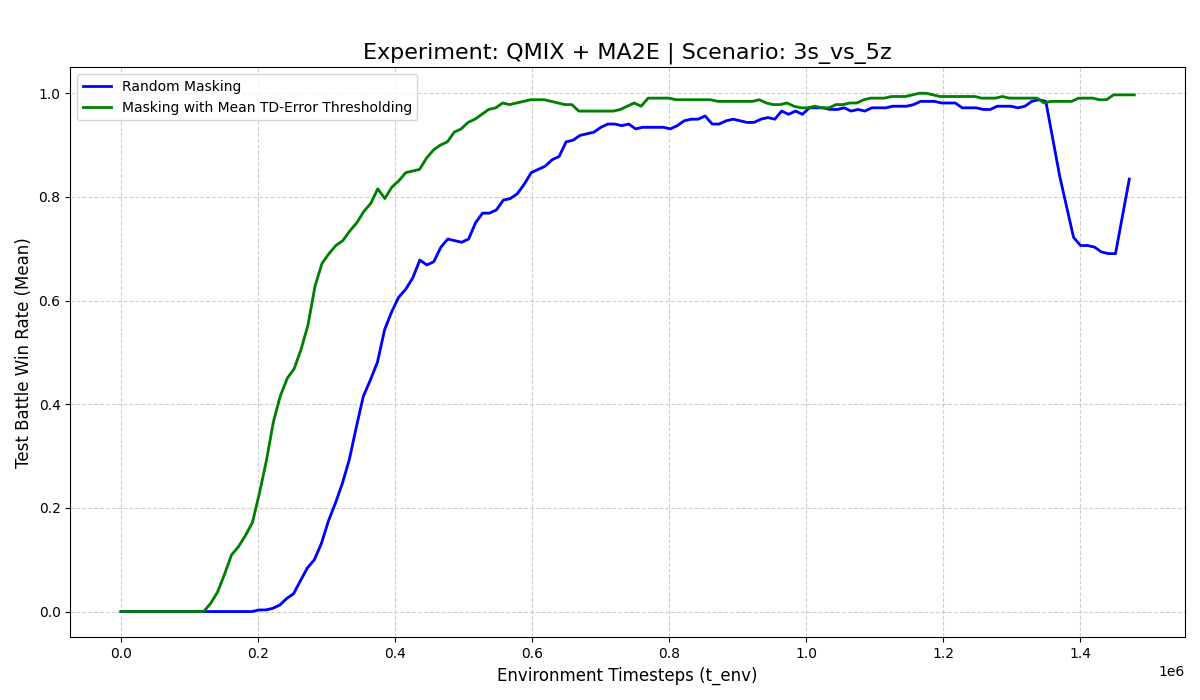
\includegraphics[width=0.8\textwidth]{images_pfe/results_li-ma2e/test_battle_won_mean_3s_vs_5z_Mean_TD-Error_Thresholding _smoothed.png}
%     \caption{Performance comparison on the \texttt{3s\_vs\_5z} HARD scenario. In this complex asymmetric task, LI-MA2E demonstrates vastly superior sample efficiency and produces a more stable final policy compared to the baseline Random Masking.}
%     \label{fig:3s_vs_5z}
% \end{figure}

% \paragraph{Analysis}
% In stark contrast to the previous map, the results on \texttt{3s\_vs\_5z} show a clear and significant advantage for our LI-MA2E framework (green line). The intelligent masking strategy leads to a dramatic improvement in both sample efficiency and final policy stability.

% LI-MA2E learns much faster, achieving a near-perfect win rate before 0.6 million timesteps, while the baseline with random masking (blue line) requires more than 1.2 million timesteps to reach a similar peak performance. Crucially, during the later stages of training (after 1.3 million steps), the baseline policy exhibits significant instability with a sharp drop in performance, a behavior not observed in our method.

% This strong result supports our core hypothesis. The \texttt{3s\_vs\_5z} map requires precise, coordinated kiting, where a single agent's mistake can be catastrophic. By adaptively focusing the MAE's reconstruction on the agent with the highest immediate error, our framework helps the team learn this essential cooperative strategy more effectively and robustly. The final stability of the LI-MA2E policy suggests that it has discovered a more general and resilient solution compared to the brittle policy learned by the baseline.

% \subsubsection{Scenario: \texttt{8m}}
% We continue our evaluation with the \texttt{8m} scenario, a symmetric map which pits \textbf{8 allied Marines against 8 enemy Marines}. This task increases the number of homogeneous agents compared to \texttt{3m} and demands effective \textbf{focus-firing} to succeed. Focus-firing is a critical coordination strategy where multiple agents target and eliminate a single enemy unit at a time. This tactic maximizes the applied damage and removes sources of enemy fire from the battlefield as quickly as possible, representing a significant coordination challenge for a multi-agent system. The results are presented in Figure~\ref{fig:8m}.

% \begin{figure}[h]
%     \centering
%     \includegraphics[width=0.8\textwidth]{images_pfe/results_li-ma2e/comparison_plot_8m.png}
%     \caption{Performance comparison on the \texttt{8m} SMAC map. Both methods converge to a perfect win rate, with the baseline showing a faster initial learning rate.}
%     \label{fig:8m}
% \end{figure}
% \paragraph{Analysis}
% Upon careful re-examination of the provided plot for the \texttt{8m} scenario, the results show a nuanced competition between the two methods. The baseline Random Masking (blue line) demonstrates a higher sample efficiency during the initial critical learning phase.

% As seen in Figure~\ref{fig:8m}, the blue line's win rate rises more steeply and consistently between 0.1 million and 0.3 million timesteps, reaching a high level of performance first. The LI-MA2E method (green line), while also learning the task, shows a noticeable dip in performance around 0.15 million timesteps and follows a slower learning trajectory in this initial phase. Both methods do eventually converge to a near-perfect win rate after approximately 1.0 million timesteps, showing that both can ultimately solve this scenario. However, the advantage in learning speed in this case belongs to the baseline.

% This finding suggests that in this specific homogeneous scenario with a larger number of agents, the broader, exploratory nature of random masking may be more effective at building a general representation than the more focused TD-error approach. This helps to define the conditions under which our LI-MA2E provides the most significant advantage—namely, in more complex, asymmetric scenarios.
\section{Main Results: Comparative Performance of $LI-{MA}^2E$}
\label{sec:main_results}

Having established the superiority of our Adaptive Mean TD-Error Thresholding strategy in the previous section, we now present a comprehensive performance evaluation of the final $LI-{MA}^2E$ framework. To validate its effectiveness and generalization capabilities, we benchmark our method against the baseline ${MA}^2E$ with random masking across a suite of challenging HARD, MEDIUM, and EASY scenarios from the SMAC environment. This section is structured to answer key research questions regarding our method's effectiveness, policy quality, and underlying learning dynamics.

\subsection{RQ1: Does Learning-Informed Masking Improve Task Completion Success?}

To answer this question, we evaluate the primary metric for task success in SMAC: the \textbf{test battle win rate}. This metric measures the percentage of episodes in which the allied agents successfully completed their objective. We present a detailed, scenario-by-scenario analysis below.
\subsubsection{Scenario: \texttt{3m}}
Our first evaluation is on the \texttt{3m} scenario, a simple symmetric map that pits \textbf{3 allied Marines against three enemy Marines}. Because  \textbf{the agents are homogeneous} and the \textbf{setup is symmetric}, the primary challenge in this map is learning a fundamental cooperative tactic: \textbf{focus-firing}. To win consistently, all three agents must learn to coordinate their attacks on the same enemy target at the same time to eliminate it quickly, rather than spreading their damage ineffectually across multiple targets. This scenario serves as a basic test of coordination. The results are presented in Figure~\ref{fig:3m}.

\begin{figure}[h]
    \centering
    \includegraphics[width=0.8\textwidth]{images_pfe/results_li-ma2e/comparison_plot_3m.png}
    \caption{Performance comparison on the \texttt{3m} SMAC map. On this simple symmetric scenario, the performance of $LI-{MA}^2E$ is comparable to the random masking baseline.}
    \label{fig:3m}
\end{figure}

\paragraph{Analysis}
As the learning curves in Figure~\ref{fig:3m} show, the performance of our $LI-{MA}^2E$ framework (green line) is largely comparable to that of the baseline ${MA}^2E$ with random masking (blue line). Both methods learn the task very rapidly, achieving a near-perfect win rate in under 250,000 environment timesteps. Throughout the remainder of the training, both policies maintain a similar high level of performance.
This result suggests that in simpler scenarios where the need for complex coordination to overcome partial observability is low, the additional guidance provided by our intelligent masking strategy does not yield a significant advantage. The baseline random masking is sufficient for the MAE module to learn the necessary representations to solve this task effectively. This provides an important baseline, demonstrating that our method's complexity does not hinder performance on easy tasks while setting the stage for evaluation on more demanding scenarios.

\subsubsection{Scenario: \texttt{3s\_vs\_3z}}
Next, we look at the \texttt{3s\_vs\_3z} scenario. In this test, our \textbf{3 agents control Stalker units}, which can attack from a distance. They face \textbf{3 enemy Zealot units}, which are severe but can only attack up close.

Because our agents can shoot from far away, the most important skill they must learn is called \textbf{kiting}. Kiting means the Stalkers must keep moving away from the chasing Zealots, while stopping briefly to shoot at them. The goal is to damage the enemy without letting them get close enough to hit back. To do this well, all three of our agents need to work together as a team. The results of this test are shown in Figure~\ref{fig:3s_vs_3z}.

\begin{figure}[h]
    \centering
    \includegraphics[width=0.8\textwidth]{images_pfe/results_li-ma2e/comparison_plot_3s_vs_3z.png}
    \caption{Performance comparison on the \texttt{3s\_vs\_3z} SMAC map. $LI-{MA}^2E$ demonstrates significantly improved sample efficiency over the baseline.}
    \label{fig:3s_vs_3z}
\end{figure}

\paragraph{Analysis}
In the \texttt{3s\_vs\_3z} scenario, the benefit of our $LI-{MA}^2E$ framework becomes immediately apparent. As shown in Figure~\ref{fig:3s_vs_3z}, the agent guided by TD-Error Masking (green line) learns significantly faster than the baseline agent using Random Masking (blue line).

Our method begins to achieve a non-zero win rate earlier, and its learning curve is considerably steeper, indicating superior sample efficiency. The $LI-{MA}^2E$ agent reaches a perfect win rate at approximately 400,000 timesteps, while the baseline requires around 600,000 timesteps to achieve the same level of performance. This result supports our hypothesis that as scenario complexity increases, an intelligent masking strategy that focuses the MAE's representational power on poorly performing agents provides a distinct advantage, enabling the system to solve the coordination task more rapidly.
\subsubsection{Scenario: \texttt{3s\_vs\_4z}}

Now, we test a harder scenario called \texttt{3s\_vs\_4z}. Here, our \textbf{3 Stalker agents}, who can shoot from a distance, must fight against \textbf{4 enemy Zealot units}, which are durable but can only attack up close.

This test is much more difficult because our agents are \textbf{outnumbered}. To win, they must use two skills together perfectly:
\begin{enumerate}
    \item \textbf{Kiting:} They must keep running away from the Zealots to stay safe, while stopping to shoot them.
    \item \textbf{Focus-Firing:} All three Stalkers must attack the \textit{same} Zealot at the same time to defeat it as quickly as possible.
\end{enumerate}
This requires excellent teamwork to succeed. The results of this difficult test are shown in Figure~\ref{fig:3s_vs_4z}.

\begin{figure}[h]
    \centering
     \includegraphics[width=0.8\textwidth]{images_pfe/results_li-ma2e/comparison_plot_3s_vs_4z.png}
    \caption{Performance comparison on the \texttt{3s\_vs\_4z} SMAC map. The plot shows a trade-off between the faster initial learning of the baseline and the more stable final convergence of $LI-{MA}^2E$.}
    \label{fig:3s_vs_4z}
\end{figure}

\paragraph{Analysis}
The \texttt{3s\_vs\_4z} scenario reveals an interesting trade-off between learning speed and final policy stability. As shown in Figure~\ref{fig:3s_vs_4z}, the baseline ${MA}^2E$ with Random Masking (blue line) exhibits a faster initial learning curve, reaching a high win rate more quickly.

However, a closer look at the convergence phase (after 0.6 million timesteps) shows that our $LI-{MA}^2E$ framework (green line) achieves a more stable and decisive convergence at a 100\% win rate. The baseline's performance, in contrast, shows more fluctuation before finally settling. This suggests that while the exploratory nature of random masking may find a working solution faster in this specific scenario, the guided approach of $LI-{MA}^2E$ produces a more robust and stable final policy.


\subsubsection{Scenario: \texttt{3s\_vs\_5z}}

Next, we test our method on \texttt{3s\_vs\_5z}, a very hard challenge from the \texttt{HARD} difficulty category. In this test, our \textbf{3 Stalker agents} (who shoot from a distance) are heavily outnumbered by \textbf{5 durable enemy Zealots} (who attack up close).

To win this difficult fight, the agents must be perfect at two skills at the same time:
\begin{enumerate}
    \item \textbf{Kiting:} They must always keep running away from the Zealots to avoid taking damage, while still turning to shoot.
    \item \textbf{Focus-Firing:} All three of our agents must attack the exact same enemy at the same time. This is the only way to defeat one of the five enemies quickly.
\end{enumerate}
This is a major test of teamwork. If even one agent makes a mistake, the team will likely lose. The agents must learn to coordinate perfectly to survive and win. The results for this difficult test are shown in Figure~\ref{fig:3s_vs_5z}.

\begin{figure}[h]
    \centering
    \includegraphics[width=0.8\textwidth]{images_pfe/results_li-ma2e/test_battle_won_mean_3s_vs_5z_Mean_TD-Error_Thresholding _smoothed.png}
    \caption{Performance comparison on the \texttt{3s\_vs\_5z} HARD scenario. In this complex asymmetric task, $LI-{MA}^2E$ demonstrates vastly superior sample efficiency and produces a more stable final policy compared to the baseline Random Masking.}
    \label{fig:3s_vs_5z}
\end{figure}

\paragraph{Analysis}
In stark contrast to the previous map, the results on \texttt{3s\_vs\_5z} show a clear and significant advantage for our $LI-{MA}^2E$ framework (green line). The intelligent masking strategy leads to a dramatic improvement in both sample efficiency and final policy stability.

$LI-{MA}^2E$ learns much faster, achieving a near-perfect win rate before 0.6 million timesteps, while the baseline with random masking (blue line) requires more than 1.2 million timesteps to reach a similar peak performance. Crucially, during the later stages of training (after 1.3 million steps), the baseline policy exhibits significant instability with a sharp drop in performance, a behavior not observed in our method.

This strong result supports our core hypothesis. The \texttt{3s\_vs\_5z} map requires precise, coordinated kiting, where a single agent's mistake can be catastrophic. By adaptively focusing the MAE's reconstruction on the agent with the highest immediate error, our framework helps the team learn this essential cooperative strategy more effectively and robustly. The final stability of the $LI-{MA}^2E$ policy suggests that it has discovered a more general and resilient solution compared to the brittle policy learned by the baseline.

\subsubsection{Scenario: \texttt{8m}}
We continue our evaluation with the \texttt{8m} scenario, a symmetric map which pits \textbf{8 allied Marines against eight enemy Marines}. This task increases the number of homogeneous agents compared to \texttt{3m} and demands effective \textbf{focus-firing} to succeed. Focus-firing is a critical coordination strategy where multiple agents target and eliminate a single enemy unit at a time. This tactic maximizes the applied damage and removes sources of enemy fire from the battlefield as quickly as possible, representing a significant coordination challenge for a multi-agent system. The results are presented in Figure~\ref{fig:8m}.

\begin{figure}[h]
    \centering
    \includegraphics[width=0.8\textwidth]{images_pfe/results_li-ma2e/comparison_plot_8m.png}
    \caption{Performance comparison on the \texttt{8m} SMAC map. Both methods converge to a perfect win rate, with the baseline showing a faster initial learning rate.}
    \label{fig:8m}
\end{figure}
\paragraph{Analysis}
Upon careful re-examination of the provided plot for the \texttt{8m} scenario, the results show a nuanced competition between the two methods. The baseline Random Masking (blue line) demonstrates a higher sample efficiency during the initial critical learning phase.

As seen in Figure~\ref{fig:8m}, the blue line's win rate rises more steeply and consistently between 0.1 million and 0.3 million timesteps, reaching a high level of performance first. The $LI-{MA}^2E$ method (green line), while also learning the task, shows a noticeable dip in performance around 0.15 million timesteps and follows a slower learning trajectory in this initial phase. Both methods do eventually converge to a near-perfect win rate after approximately 1.0 million timesteps, showing that both can ultimately solve this scenario. However, the advantage in learning speed in this case belongs to the baseline.

This finding suggests that in this specific homogeneous scenario with a larger number of agents, the broader, exploratory nature of random masking may be more effective at building a general representation than the more focused TD-error approach. This helps to define the conditions under which our $LI-{MA}^2E$ provides the most significant advantage, namely, in more complex, asymmetric scenarios.


\paragraph{Answer to RQ1:}
In summary, the evidence shows that the answer to this question is \textbf{yes, particularly in complex, asymmetric scenarios.} While the performance of $LI-{MA}^2E$ is comparable on simple maps, it demonstrates significantly improved sample efficiency and final policy stability on complex maps like \texttt{3s\_vs\_5z}. This suggests that our method yields more reliable task completion when coordination is most critical.

%----------------------------------------------------------------------------------------
\subsection{RQ2: Does Our Masking Lead to Higher-Quality Policies?}
%----------------------------------------------------------------------------------------

Beyond simply winning, a superior algorithm should learn to win more efficiently. To investigate this, we analyze the \textbf{mean test return}. This metric reflects the \textit{quality} and \textit{efficiency} of the learned policy, where a higher return often corresponds to winning with more surviving units or in less time.


\begin{figure}[h]
    \centering
    % Row 1 of plots
    \subfloat[Scenario: 3m]{\includegraphics[width=0.32\textwidth]{images_pfe/results_test_return_mean/comparison_plot_3m.png}
    \label{fig:3m_return}}
    \hfill
    \subfloat[Scenario: 3s\_vs\_3z]{\includegraphics[width=0.32\textwidth]{images_pfe/results_test_return_mean/comparison_plot_3s_vs_3z.png}
    \label{fig:3s_vs_3z_return}}
    \hfill
    \subfloat[Scenario: 3s\_vs\_4z]{\includegraphics[width=0.32\textwidth]{images_pfe/results_test_return_mean/comparison_plot_3s_vs_4z.png}\label{fig:3s_vs_4z_return}}
    
    \vspace{1em} % Adds a little vertical space between rows
    
    % Row 2 of plots
    \subfloat[Scenario: 3s\_vs\_5z]{\includegraphics[width=0.32\textwidth]{images_pfe/results_test_return_mean/comparison_plot_3s_vs_5z.png}\label{fig:3s_vs_5z_return}}
    \hfill
    \subfloat[Scenario: 8m]{\includegraphics[width=0.32\textwidth]{images_pfe/results_test_return_mean/comparison_plot_8m.png}\label{fig:8m_return}}
    
    \caption{Mean test return for $LI-{MA}^2E$ (green) vs. baseline Random Masking (blue) across various SMAC scenarios. This metric shows the quality and efficiency of the learned policies.}
    \label{fig:all_returns}
\end{figure}
\paragraph{Analysis}
In scenarios such as \texttt{3s\_vs\_3z} and \texttt{3s\_vs\_4z}, our TD-Error Masking (green line) rapidly converges to the maximum possible return, while the baseline Random Masking (blue line) plateaus at a significantly lower, suboptimal level. Notably, in the \texttt{3s\_vs\_4z} scenario, while the baseline previously appeared to learn faster based on win rate, this more sensitive metric reveals that $LI-{MA}^2E$ learned the correct, high-reward strategy almost immediately, indicating a much higher policy quality. This advantage extends to the most difficult maps like \texttt{3s\_vs\_5z}, where  $LI-{MA}^2E$ not only achieves a higher return faster but also maintains a more stable final policy, avoiding the sharp performance drops exhibited by the baseline. Even on homogeneous maps like \texttt{3m} and \texttt{8m}, our method reaches the optimal return with greater speed and stability. Collectively, this strong evidence supports the conclusion that our intelligent masking strategy does not just help agents learn \textit{to} win, but guides them to learn \textit{how to win optimally}, producing more robust and efficient cooperative policies across a wide range of challenges.

\paragraph{Answer to RQ2:}
The evidence provides a decisive \textbf{yes}. Across all tested scenarios, the mean test return plots show that  $LI-{MA}^2E$ consistently learns higher-quality policies much more quickly than the baseline. 
\subsection{RQ3: What Are the Underlying Learning Dynamics?}
%----------------------------------------------------------------------------------------

\paragraph{Answer to RQ3 (Summary and Pointer to Appendix):}
The superior performance in both task completion and policy quality is a direct result of a more stable and efficient learning process. A detailed analysis of the underlying learning dynamics, presented in \textbf{Appendix~\ref{app:td_error_abs_analysis}}, directly addresses this question by examining the mean absolute TD-error. The analysis shows that our $LI-{MA}^2E$ framework is consistently more effective at reducing and stabilizing the agents' prediction errors, providing a mechanistic explanation for the observed performance gains.
\section*{Conclusion}

This chapter presented a comprehensive empirical validation of our proposed Learning-Informed Masking Framework. The experimental journey began with a methodical investigation into several candidate scoring functions, culminating in the selection of the \textbf{Adaptive Mean TD-Error Thresholding} strategy as the most robust and effective approach. The subsequent comparative analysis against the baseline framework provided strong empirical support for our central hypothesis. The results demonstrated that  $LI-{MA}^2E$ leads to more reliable \textbf{task completion (Win Rate)} and consistently produces \textbf{higher-quality and more efficient policies (Mean Test Return)}. The underlying mechanism for these improvements (a more stable and efficient learning process ) was substantiated by a direct analysis of the TD-error dynamics in the appendix. Collectively, the evidence confirms that an intelligent, learning-informed masking curriculum is superior to a random one, not only in achieving victory but in the quality and robustness of the strategies learned.

% \paragraph{Perspectives}
% The nuanced results from this chapter also open up several promising perspectives for future research. The varying performance of our method across different SMAC maps suggests that the optimal masking strategy may be scenario-dependent. A significant future direction would be to develop a meta-learning framework where the masking strategy itself (e.g., the choice of score or its hyperparameters) is adapted based on the detected characteristics of the environment. Furthermore, while TD-error proved to be a robust signal, future work could explore incorporating other information sources into the scoring function. Signals from credit assignment methods or even learned communication protocols could potentially provide an even richer, more context-aware metric for identifying the most critical agents to mask. These perspectives highlight how the principle of learning-informed masking can serve as a foundation for even more sophisticated and adaptive multi-agent learning systems.





\chapter{General Conclusion and Perspectives}
\label{chap:general_conclusion}
\addcontentsline{toc}{chapter}{General Conclusion and Perspectives}

\section*{General Conclusion}

This project looked at a major challenge in multi-agent reinforcement learning: how can a team of agents work together effectively when they can only see a small part of their environment? We saw that current methods, like the ${MA}^2E$ framework, use a random masking approach to help agents learn about the wider world. However, this random approach has a key weakness: it is disconnected from how well the agents are actually learning to play the game.

To fix this, we created and tested a new method called the \textbf{Learning-Informed Masking Framework ($LI-{MA}^2E$)}. The main idea is to use an agent's own performance during training to intelligently decide who to mask. We tested several different ways to score agents and found that a simple strategy based on the team's average TD-error worked best.

Our experiments showed that this idea is very effective. Compared to the baseline, our $LI-{MA}^2E$ method helped agents:
\begin{itemize}
    \item \textbf{Win more reliably and learn much faster}, especially on difficult maps where teamwork is critical.
    \item \textbf{Learn to win in a better, more efficient way}, achieving higher scores (mean test return) and more stable final strategies.
\end{itemize}
The reason for this success is that our method creates a more stable and focused learning process, as shown by the analysis of the TD-error. In short, our work proves that connecting the masking task directly to the agent's learning progress is a powerful way to improve teamwork in MARL.

\section*{Perspectives}

The results from this project also point to several exciting ideas for future research.

\begin{itemize}
    \item \textbf{Smarter, Adaptive Masking:} We noticed that our method's performance sometimes changed depending on the map. A great next step would be to create a system that can automatically learn and adapt its masking strategy for each new challenge it faces.

    \item \textbf{Exploring New Scoring Methods:} While TD-error worked very well, other signals could also be used to identify struggling agents. Future work could explore using metrics related to an agent's contribution to the team's success or even information from communication signals to create an even more powerful scoring function.

    \item \textbf{Real-World Applications:} The principles of $LI-{MA}^2E$ are general. It would be very valuable to test this framework outside of the StarCraft game environment, for example, with real-world applications like coordinating swarms of search-and-rescue drones or managing teams of robots in a warehouse.
\end{itemize}
\appendix
\appendixpage
\pagenumbering{roman}

\chapter{Definitions}

\label{app:definitions}

- \textbf{Fully-cooperative settings}: refer to scenarios in which all participants or agents involved are aligned towards achieving a common goal. In these settings, the success of the collective effort is prioritized over individual gains, and the participants work together seamlessly, sharing resources, information, and strategies to maximize the overall outcome.

% - \textbf{Semi-cooperative settings}: refer to scenarios where participants or agents share a partial alignment towards common goals but retain some level of individual objectives or competition.

% - \textbf{Coverage}: refers to the geographic area on the Earth's surface that a satellite can observe, monitor, or communicate with at any given time.


- \textbf{Environment}: An environment is a physical or virtual world whose state
evolves over time and is influenced by the actions of the agents that exist
within the environment. The environment specifies the actions that agents
can take at any point in time, as well as the observations that individual
agents receive about the state of the environment. The states of the environment may be defined as discrete or continuous quantities, or a combination
of both.

-\textbf{Agents}: An agent is an entity which receives information about the state of the
environment and can choose different actions in order to influence the state.
Agents may have different prior knowledge about the environment, such as
the possible states that the environment can be in and how states are affected
by the actions of the agents. Importantly, agents are goal-directed in the
sense that agents have specified goals and choose their actions in order to
achieve their goals.

- \textbf{Policy}: refers to a function used by the agent to select actions (or assign probabilities to selecting each action) given the current state of the environment. If the environment is only partially observed
by the agent, then the policy may be conditioned on the current and past
observations of the agent.

- \textbf{MARL:} a multi-agent system consists of an environment and multiple decision-making
agents that interact in the environment to achieve certain goals.

- \textbf{Finite Markov decision process}: A finite Markov decision process
(MDP) consists of: 
\begin{itemize}
    \item Finite set of states S, with subset of terminal states $\Bar{S} \subset S$
    \item  Finite set of actions A
    \item Reward function R : $S × A × S \rightarrow R$
    \item State transition probability function $T : S × A × S \rightarrow [0, 1]$ such that:
    \begin{equation}
    \forall s \in S, a \in A: \sum_{s' \in S} T(s,a,s') = 1
\end{equation}
    \item Initial state distribution $\mu : S \rightarrow [0, 1]$ such that:
\begin{equation}
    \sum _{s \in S} \mu (s) = 1\  \text{and} \ \forall s \in \Bar{S}: \mu (s) =0 \end{equation}
\end{itemize}


% - \textbf{Event-Triggered Mechanism:} Coordination and control of agents based on specific events or changes in the system's state (like the \textbf{local event detection}: change in state (battery, robotics..), detection of byzantine agents or \textbf{threshold-based triggering}: based on distance or reputation of agents).

% - \textbf{Formation Control: }Coordination and Control of a group of autonomous agents to achieve and maintain a desired geometric configuration. It can be centralized (a central controller guides the entire formation) or decentralized (each entity makes decisions based on local observations).

% - \textbf{Leader Tracking:} Capability of a system to monitor and follow the movements or actions of a designated dynamic leader.


- \textbf{Stochastic Model: } a mathematical approach that incorporates random variables to predict a range of possible outcomes rather than a single deterministic result. It accounts for inherent uncertainties and variability in the system being modeled.


- \textbf{Deterministic Model: }a mathematical approach that predicts a single, specific outcome given a set of initial conditions. It assumes no randomness in the system, so the results are entirely determined by the input parameters.




- \textbf{Greedy policies}: A policy is greedy with respect to a value function it is optimal according to that value function for a one-step problem.



    
\newpage
\chapter{Extended Background}
\label{app:extended_background}
\section{The Multi-Agent Transformer (MAT)}
\label{sec:MAT}

 is a novel encoder-decoder architecture designed to treat cooperative multi-agent reinforcement learning (MARL) as a sequence modeling problem. The core idea is to map a sequence of agent observations $(o_{i_1}, \dots, o_{i_n})$ to a sequence of optimal actions $(a_{i_1}, \dots, a_{i_n})$.

\textbf{Overall Architecture: } As illustrated in  Figure~\ref{fig:mat_architecture}, the MAT architecture is structured as an encoder-decoder model. This design is not arbitrary; it's a direct implementation of the \textbf{Multi-Agent Advantage Decomposition Theorem}. This theorem is the cornerstone of the entire approach, stating that the advantage of a joint action can be decomposed into a sum of local, ordered advantages:
\begin{equation}
    \label{eq:mat_advantage_decomp}
    A_{\pi_{i_{1:n}}}(o, a_{i_{1:n}}) = \sum_{m=1}^{n} A_{\pi_{i_m}}(o, a_{i_{1:m-1}}, a_{i_m})
\end{equation}
This decomposition transforms the complex joint policy optimization into a sequential decision-making process, where each agent's decision is conditioned on the actions of its predecessors in a given permutation. The MAT architecture is designed to explicitly model this sequential dependency.

\textbf{Encoder: Multi-Agent Observation Encoding: } The first stage, the Multi-Agent Observation Encoding block shown in the top half of the diagram, serves as the encoder. Its primary function is to process the joint observations and learn expressive latent representations $(\hat{o}_{i_1}, \dots, \hat{o}_{i_n})$ that capture the complex interrelationships between agents. It uses standard Transformer blocks composed of self-attention and MLPs to achieve this.

Crucially, during training, the encoder is also optimized to learn the agents' value functions. This is accomplished by minimizing the empirical Bellman error via the following loss function:
\begin{equation}
    \label{eq:mat_encoder_loss}
    L_{\text{Encoder}}(\phi) = \frac{1}{Tn} \sum_{m=1}^{n} \sum_{t=0}^{T-1} \left[ R(o_t, a_t) + \gamma V_{\phi'}(\hat{o}_{t+1}^{i_m}) - V_{\phi}(\hat{o}_{t}^{i_m}) \right]^2
\end{equation}
Here, $V_{\phi}$ is the value function parameterized by the encoder's weights $\phi$, and $\phi'$ represents the parameters of a frozen target network, a standard technique for stabilizing training.

\textbf{Decoder: Auto-regressive Action Decoding:} The second stage is the Auto-regressive Action Decoding block, which generates an optimal action for each agent sequentially. This directly implements the sequential dependency from the decomposition theorem. As shown in the bottom half of the diagram, the decoder receives the latent observation representations from the encoder and the sequence of previously generated actions.

Its auto-regressive nature means the policy for agent $i_m$ is conditioned on the latent joint observation and the actions of preceding agents: $\pi_{\theta_{i_m}}(a_{i_m} | \hat{o}_{i_{1:n}}, a_{i_{1:m-1}})$. This is enforced by a masked self-attention mechanism, which ensures that the computation for agent $i_m$ can only attend to the outputs of agents $i_1, \dots, i_{m-1}$.

To train the decoder parameters $\theta$, MAT uses a clipping objective from Proximal Policy Optimization (PPO):
\begin{equation}
    \label{eq:mat_decoder_loss}
    L_{\text{Decoder}}(\theta) = -\frac{1}{Tn} \sum_{m=1}^{n} \sum_{t=0}^{T-1} \min \left( r_t^{i_m}(\theta)\hat{A}_t, \text{clip}(r_t^{i_m}(\theta), 1 \pm \epsilon)\hat{A}_t \right)
\end{equation}
The policy ratio is $r_t^{i_m}(\theta) = \frac{\pi_{\theta_{i_m}}(a_{t}^{i_m} | \hat{o}_{t}^{i_{1:n}}, a_{t}^{i_{1:m-1}})}{\pi_{\theta_{\text{old}}}(a_{t}^{i_m} | \hat{o}_{t}^{i_{1:n}}, a_{t}^{i_{1:m-1}})}$, and $\hat{A}_t$ is an estimate of the joint advantage function, calculated using Generalized Advantage Estimation (GAE) with the value function from the encoder as a baseline.

This design provides a monotonic improvement guarantee while also being highly computationally efficient, as it allows for parallel computation of losses during training (since actions are known from the replay buffer). During inference, actions are generated one by one, as shown by the red dashed feedback loop in the diagram.

\begin{figure}[H]
  \centering
 \includegraphics[width=0.75\textwidth]{img_pfe/MAT_arch.PNG}
  \caption{The encoder-decoder architecture of MAT. At each time step, the encoder takes in a sequence of
agents’ observations and encodes them into a sequence of latent representations, which is then passed into
the decoder. The decoder generate each agent’s optimal action in a sequential and auto-regressive manner.
The masked attention blocks ensures agents can only access its preceding agents’ actions during training. (adapted from \parencite{MAT} )}
\label{fig:mat_architecture}
\end{figure}
\FloatBarrier

\section{The Multi-Agent Decision Transformer (MADT)}
\label{sec:MADT}
  Is a novel approach designed to leverage large, offline datasets to pre-train a single, generalizable policy for multi-agent reinforcement learning (MARL) tasks. The core idea is to first treat MARL as a sequence modeling problem for offline pre-training and then fine-tune this model in an online environment to improve performance and sample efficiency. The entire pipeline, as illustrated in the paper's Figure~\ref{fig:madt_architecture}, consists of these two main phases: offline pre-training on static data followed by online fine-tuning through active interaction. The ultimate goal is to create a universal policy that can generalize across different scenarios and tasks with strong few-shot and zero-shot capabilities.

In the offline phase, detailed on the left side of the provided diagram, MADT casts the problem as a conditional sequence modeling task using a Causal Transformer to autoregressively predict an agent's actions based on past events. The learning process uses trajectories where each step is a token $x_t$ composed of the global state, local observation, and action, $x_t = (s_t, o_t^i, a_t^i)$. Notably, this formulation omits the \textit{reward-to-go} signal, as ablation studies found it harmful to online performance. To ensure predictions at timestep $t$ only depend on past inputs, the architecture uses a lower triangular mask $M$ in its attention mechanism, calculated as:
\begin{equation}
\label{eq:madt_att}
    \text{Attention}(Q,K,V) = \text{softmax}\left(\frac{QK^T}{\sqrt{d_k}} + M\right)V
\end{equation}
This offline model is trained with a supervised Cross-Entropy (CE) loss, $L_{\text{CE}}(\theta) = \frac{1}{C} \sum P(a_t) \log P(\hat{a}_t|\tau_t, \hat{a}_{<t}; \theta)$, to imitate the behavior in the dataset.

Since this imitation learning lacks the incentive to maximize rewards, the model then transitions to an online fine-tuning stage. In this phase, as shown on the right side of the diagram, the pre-trained Causal Transformer serves as a shared backbone for separate Actor and Critic networks within a Proximal Policy Optimization (PPO) framework. The Actor network's parameters $\theta_i$ are updated by maximizing the PPO clip objective:
\begin{equation*}
    \theta_i \leftarrow \arg\max_{\theta_i} \mathbb{E}\left[\min\left(w_t(\theta_i) A(s,a_i), \text{clip}(w_t(\theta_i), 1-\epsilon, 1+\epsilon)A(s, a_i)\right)\right]
\end{equation*}
where $w$ is the importance sampling weight. The Critic network's parameters $\phi$ are updated by minimizing the Mean Squared Error (MSE) loss:
\begin{equation}
 \label{eq:madt_loss}
    L_{\phi} = \frac{1}{2} \left( \sum_t \gamma^t r_t - V_{\phi}(s) \right)^2
\end{equation}
% This two-stage process allows MADT to learn a strong prior and then rapidly adapt to maximize rewards, boosting sample efficiency. To ensure the model can generalize across scenarios, it employs several key techniques:
% \begin{itemize}
%     \item Parameter sharing across agents with a one-hot agent ID.
%     \item Feature encoding by padding features to a universal size.
%     \item Action masking to handle different action spaces.
%     \item Reward scaling to balance learning across tasks.
% \end{itemize}
This two-stage process boosts sample efficiency and enables generalization across scenarios through key techniques like parameter sharing, feature padding, action masking, and reward scaling.
\begin{figure}[H]
  \centering
 \includegraphics[width=0.75\textwidth]{img_pfe/MADT_arch.PNG}
  \caption{The detailed model structure for offline and online MADT (adapted from \parencite{MADT})}
\label{fig:madt_architecture}
\end{figure}

\section{Formalism of Common Knowledge}
\label{sec:mackrl_details}
\textbf{Common Knowledge in Multi-Agent Systems: } Common knowledge of a group of agents ${\mathcal{G}}$ refers to facts that all members know, and that each individual knows that all other individuals know it, each individual knows that all other individuals know that all the individuals know it, and so on. Any data $\xi$ that are known to all agents before execution/training, like a shared random seed, are obviously common knowledge. Crucially, every agent $a \in {\mathcal{G}}$ can deduce the same history of common knowledge $\tau_t^{\mathcal{G}}$ from its own history $\tau_t^a$ and the commonly known data $\xi$, that is, $\tau_t^{\mathcal{G}} := I_{\mathcal{G}}(\tau_t^a, \xi) = I_{\mathcal{G}}(\tau_t^{\bar{a}}, \xi)$, for all $a, \bar{a} \in {\mathcal{G}}$.

Furthermore, any actions taken by a policy $\pi_{\mathcal{G}}(u_{\text{env}}^{\mathcal{G}} | \tau_t^{\mathcal{G}})$ over the group’s joint action space $U_{\text{env}}^{\mathcal{G}}$ are themselves common knowledge, if the policy is deterministic or pseudo-random with a shared random seed and conditions only on the common history $\tau_t^{\mathcal{G}}$. Common knowledge of subgroups ${\mathcal{G}}_0 \subset \mathcal{G}$ cannot decrease, that is, $I_{{\mathcal{G}}_0}(\tau_t^a, \xi) \supseteq I_{\mathcal{G}}(\tau_t^a, \xi)$.

\textbf{Common Knowledge with Uncertainty:} Given a Dec-POMDP with noisy observations, agents in a group $\mathcal{G}$ might not be able to establish true common knowledge even if sensor noise properties are commonly known \parencite{knowledge_common_knowledge_distributed_env}. Instead, each agent $a$ can only deduce its own beliefs $\tilde{I}_a^{\mathcal{G}}(\tilde{\tau}_t^a)$ over what is commonly known within $\mathcal{G}$, where $\tilde{\tau}_t^a$ is the agent’s belief over what constitutes the groups’ common history. Each agent $a$ can then evaluate its own belief over the group policy $\tilde{\pi}_a^{\mathcal{G}}(u_{\text{env}}^{\mathcal{G}} | \tilde{\tau}_t^{\mathcal{G}})$. In order to minimize the probability of disagreement during decentralized group action selection, agents in $\mathcal{G}$ can perform optimal correlated sampling based on a shared random seed.

\textbf{Learning under common knowledge (LuCK):} is a  cooperative multi-agent reinforcement learning setting, where a Dec-POMDP is augmented by a common knowledge function $I_{\mathcal{G}}$ (or probabilistic common knowledge function $\tilde{I}_a^{\mathcal{G}}$). Groups of agents ${\mathcal{G}}$ can coordinate by learning policies that condition on their common knowledge. In this paper $I_{\mathcal{G}}$ (or $\tilde{I}_a^{\mathcal{G}}$) is fixed a priori, but it could also be learnt during training. The setting accommodates a wide range of real-world and simulated multi-agent tasks. Whenever a task is cooperative and learning is centralised, then agents can naturally learn suitable $I_{\mathcal{G}}$ or $\tilde{I}_a^{\mathcal{G}}$. Policy parameters can be exchanged during training as well and thus become part of the commonly known data $\xi$. Joint policies where coordinated decisions of a group ${\mathcal{G}}$ only condition on the common knowledge of ${\mathcal{G}}$ can be executed in a fully decentralised fashion.

\textbf{Field-of-View Common Knowledge:} is a form of complete-history common knowledge \parencite{knowledge_common_knowledge_distributed_env}, that arises within a Dec-POMDP if agents can deduce parts of other agents’ observations from their own. In this case, an agent group’s common knowledge is the intersection of observations that all members can reconstruct from each other. under some assumptions, common knowledge is the intersection of all agents’ sets of visible objects, if and only if all agents can see each other. This naturally occurs in many interesting real-world tasks, such as autonomous driving and robo-soccer \parencite{robot_soccer}.
\newpage
% \chapter{Analysis of Learning Stability}
% \section{Analysis of Mean Absolute TD-error metric}
% \label{app:td_error_abs_analysis}

% This appendix provides a direct analysis of the learning process by visualizing the mean absolute TD-error. This metric offers insight into the stability and convergence of the agents' underlying value functions. A lower, more stable TD-error indicates that the agents are making more accurate predictions and have learned a more reliable policy. The following plots compare our LI-MA2E framework against the baseline Random Masking across the tested SMAC scenarios.

% %-------------------------------------------------
% \subsection{Scenario: \texttt{3m}}
% %-------------------------------------------------

% \begin{figure}[H]
%     \centering
%     \includegraphics[width=0.8\textwidth]{images_pfe/results_td_error_abs/comparison_plot_3m.png}
%     \caption{Mean absolute TD-error on the \texttt{3m} scenario.}
%     \label{fig:3m_td_error}
% \end{figure}

% \paragraph{Analysis}
% In the \texttt{3m} scenario, the TD-error for the Random Masking baseline (blue line) starts low but spikes dramatically after 3000 timesteps, indicating a period of high instability as it learns. In contrast, our LI-MA2E method (green line) maintains a consistently lower and more stable TD-error throughout the same period. This suggests that our intelligent masking curriculum helps prevent these learning instabilities.

% %-------------------------------------------------
% \subsection{Scenario: \texttt{8m}}
% %-------------------------------------------------

% \begin{figure}[H]
%     \centering
%     \includegraphics[width=0.8\textwidth]{images_pfe/results_td_error_abs/comparison_plot_8m.png}
%     \caption{Mean absolute TD-error on the \texttt{8m} scenario.}
%     \label{fig:8m_td_error}
% \end{figure}

% \paragraph{Analysis}
% The TD-error plot for the \texttt{8m} scenario shows a similar trend. The Random Masking baseline (blue line) exhibits a large spike in error around 3400 timesteps, signifying a significant learning challenge. Our LI-MA2E framework (green line), however, maintains a much more stable and consistently lower TD-error, effectively navigating the learning process without the same degree of instability.

% %-------------------------------------------------
% \subsection{Scenario: \texttt{3s\_vs\_3z}}
% %-------------------------------------------------

% \begin{figure}[H]
%     \centering
%     \includegraphics[width=0.8\textwidth]{images_pfe/results_td_error_abs/comparison_plot_3s_vs_3z.png}
%     \caption{Mean absolute TD-error on the  \texttt{3s\_vs\_3z} scenario.}
%     \label{fig:3s_vs_3z_td_error}
% \end{figure}

% \paragraph{Analysis}
% In the  \texttt{3s\_vs\_3z} scenario, the initial TD-error for the baseline (blue line) is very high before it sharply drops and stabilizes at a low value. Our LI-MA2E method (green line) shows a more controlled descent, and while it exhibits more variance, it consistently pushes the error to a lower floor than the baseline after 3000 timesteps. This demonstrates a more effective error reduction in the long run.

% %-------------------------------------------------
% \subsection{Scenario: \texttt{3s\_vs\_4z}}
% %-------------------------------------------------

% \begin{figure}[H]
%     \centering
%     \includegraphics[width=0.8\textwidth]{images_pfe/results_td_error_abs/comparison_plot_3s_vs_4z.png}
%     \caption{Mean absolute TD-error on the `3s\_vs\_4z` scenario.}
%     \label{fig:3s_vs_4z_td_error}
% \end{figure}

% \paragraph{Analysis}
% The results on  \texttt{3s\_vs\_4z} are particularly telling. The baseline's TD-error (blue line) remains stubbornly high for a long period before slowly decreasing. In contrast, the LI-MA2E's TD-error (green line), while initially volatile, is driven down much more effectively and consistently remains at a lower level than the baseline. This directly supports the finding that LI-MA2E learns a higher-quality policy, as it is more successful at minimizing the underlying prediction error.

% %-------------------------------------------------
% \subsection{Scenario: \texttt{3s\_vs\_5z}}
% %-------------------------------------------------

% \begin{figure}[H]
%     \centering
%     \includegraphics[width=0.8\textwidth]{images_pfe/results_td_error_abs/comparison_plot_3s_vs_5z.png}
%     \caption{Mean absolute TD-error on the \texttt{3s\_vs\_5z} scenario.}
%     \label{fig:3s_vs_5z_td_error}
% \end{figure}

% \paragraph{Analysis}
% On the difficult \texttt{3s\_vs\_5z} map, our LI-MA2E method (green line) again demonstrates its ability to control and reduce error more effectively than the baseline (blue line). After an initial spike, the green line is consistently suppressed, while the blue line remains higher for longer. This shows that by focusing on the agents with high error, our method creates a curriculum that actively minimizes that error across the team, leading to a more stable and efficient learning process. This stability is the reason LI-MA2E achieves higher returns and avoids the policy degradation seen in the baseline.
\chapter{Analysis of Learning Stability}
\section{Analysis of Mean Absolute TD-error}
\label{app:td_error_abs_analysis}

This appendix provides a direct analysis of the learning process by visualizing the mean absolute TD-error. This metric offers insight into the stability and convergence of the agents' underlying value functions. A lower, more stable TD-error indicates that the agents are making more accurate predictions and have learned a more reliable policy. Figure~\ref{fig:all_td_errors} compares our LI-MA2E framework against the baseline Random Masking across the tested SMAC scenarios.

\begin{figure}[H]
    \centering
    % Row 1 of plots
    \subfloat[Scenario: \texttt{3m}]{\includegraphics[width=0.32\textwidth]{images_pfe/results_td_error_abs/comparison_plot_3m.png}\label{fig:3m_td_error}}
    \hfill
    \subfloat[Scenario: \texttt{8m}]{\includegraphics[width=0.32\textwidth]{images_pfe/results_td_error_abs/comparison_plot_8m.png}\label{fig:8m_td_error}}
    \hfill
    \subfloat[Scenario: \texttt{3s\_vs\_3z}]{\includegraphics[width=0.32\textwidth]{images_pfe/results_td_error_abs/comparison_plot_3s_vs_3z.png}\label{fig:3s_vs_3z_td_error}}
    
    \vspace{1em} % Adds a little vertical space between rows
    
    % Row 2 of plots
    \subfloat[Scenario: \texttt{3s\_vs\_4z}]{\includegraphics[width=0.32\textwidth]{images_pfe/results_td_error_abs/comparison_plot_3s_vs_4z.png}\label{fig:3s_vs_4z_td_error}}
    \hfill
    \subfloat[Scenario: \texttt{3s\_vs\_5z}]{\includegraphics[width=0.32\textwidth]{images_pfe/results_td_error_abs/comparison_plot_3s_vs_5z.png}\label{fig:3s_vs_5z_td_error}}
    
    \caption{Mean absolute TD-error for LI-MA2E (green) vs. baseline Random Masking (blue) across various SMAC scenarios.}
    \label{fig:all_td_errors}
\end{figure}

\paragraph{Analysis}
The mean absolute TD-error plots in Figure~\ref{fig:all_td_errors} provide a clear and consistent insight into the learning dynamics of our $LI-MA^2E$ framework compared to the baseline. Across all scenarios, our intelligent masking strategy leads to a more stable and effective learning process. In the homogeneous maps \texttt{3m} and \texttt{8m}, the baseline method exhibits dramatic spikes in TD-error during training, indicating periods of high instability. Our $LI-MA^2E$ method, in contrast, maintains a consistently lower and more stable error, suggesting it helps prevent such instabilities. In more complex scenarios like \texttt{3s\_vs\_4z}  and \texttt{3s\_vs\_5z}, the baseline's TD-error remains stubbornly high for longer periods, whereas $LI-MA^2E$ is able to control and suppress the error much more effectively. This demonstrates that by actively focusing the MAE's reconstruction on agents with high prediction error, our framework creates a curriculum that directly and efficiently minimizes that error across the team. This more stable learning process is the underlying reason for the superior policy quality and performance gains detailed in the main results chapter.
% \chapter{Algorithms}

% \section*{Iterative Policy Evaluation Algorithm}
% \begin{algorithm}[H]
%     \caption{Iterative Policy Evaluation Algorithm}
%     \begin{algorithmic}[1]
%         \State Initialize $V(s) = 0$ for all $s \in \mathcal{S}$ (or arbitrarily)
%         \State $\theta > 0$ (a small threshold)
%         \State $\gamma$ (discount factor) where $0 \leq \gamma \leq 1 $
%         \Repeat
%             \State $\Delta \leftarrow 0$
%             \For{each state $s \in \mathcal{S}$}
%                 \State $v \leftarrow V(s)$
%                 \State $V(s) \leftarrow \sum_{a} \pi(a|s) \sum_{s', r} p(s', r|s, a) \left[ r + \gamma V(s') \right]$
%                 \State $\Delta \leftarrow \max(\Delta, |v - V(s)|)$
%             \EndFor
%         \Until{$\Delta < \theta$}
%     \end{algorithmic}
% \end{algorithm}



% \section*{Value Iteration Algorithm}
% \begin{algorithm}[H]
%     \caption{VALUE ITERATION}
%     \label{alg:value_iteration}
%     \begin{algorithmic}
%         \State \textbf{Initialize} \(V_0(s)\) arbitrarily (often set to 0 for all states)
        
%         \For{each iteration \(k\)}
      
%        \For{each state \(s \in \mathcal{S}\)}
           
%                 \State Update the value function \(V_{k+1}(s)\) using the Bellman equation:
%                 \[
%                 V_{k+1}(s) = \max_{a \in \mathcal{A}} \sum_{s' \in \mathcal{S}} P(s'|s, a) \left[ R(s, a, s') + \gamma V_k(s') \right]
%                 \]
%             \EndFor
            
%             \State Check for convergence: if the change in value function is smaller than a predefined threshold, stop
%         \EndFor
%     \end{algorithmic}
% \end{algorithm}




% \section*{Peer Evaluation based dual DQN Algorithm}

%     \begin{algorithm}[H]
%         Initialize replay memory, $[Q_a ^{A}]$, $[Q_a ^{M}]$, and the target with random parameters.
%         \\ 
%         for \ episode < max-ep do
%         \\
%         \hspace*{0.5cm} Make \ observations
%         \\
%         \hspace*{0.5cm} for \ t$<$time-steps:
%         \\
%         \hspace*{0.9cm} select\  action \ using \ $\epsilon - greedy$
%         \\
%         \hspace*{0.9cm} retrieve \ next observation \  and \  reward 
%         \\
%         \hspace*{0.9cm} calculate \  peer \ evaluation \  $z_a ^t$ \ for \  each \ agent \ $a$
%         \\
%         \hspace*{0.9cm} identify \ peers \ $K_a$ \ and \ aggregate \ the \ peer \ evaluations
%         \\
%         \hspace*{0.9cm} Store \ transition \ $(o^t, u^t, r^t, o^{t+1}, Z^t)$ \ in \ D
%         \\
%         \hspace*{0.9cm} \textbf{if} \ t$>$ warm-up-period \ \textbf{then:}
%         \\
%         \hspace*{1.2cm} $\hat{r} _a = r_a + \beta Z_a$ for each agent a 
%         \\
%         \hspace*{0.9cm} \textbf{end if}
%         \\ 
%         \hspace*{0.5cm} For each agent, update Neural Networks by minimizing the loss: 
%         \\
%         \hspace*{1.2cm} $L_a ^{A} (o_a, u_a, r_a, o'_a | \theta _a ^{A} , \theta _a ^{A'} = \sum ( Q^{A} (o,u | \theta _a ^{A} - y_a^{A} (o', r | \theta _a ^{A'}))^2$

%         \caption{Peer Evaluation based Dual DQN Training Algorithm}
%     \end{algorithm}



% \section*{Introspective Learning Algorithm}
% \begin{algorithm}[H]
%     \caption{INTROSPECTION LEARNING}
%     \label{alg:introspection_learning}
%     \begin{algorithmic}[1]
%         \State \textbf{Data:} Off-policy RL algorithm OPRL, policy function $\pi$, family of queries $(U_i)_i$, a schedule $\sigma$, a reward cutoff $R$
        
%         \State Initialize OPRL policy $\pi$ with random weights $\vartheta$ and replay buffer $D$
        
%         \For{episode $e \in \{1, \ldots, M\}$}
        
%         \hspace*{0.4cm}    \State Train OPRL as specified
            
%            \hspace*{0.4cm} \If{moving average reward $< R$ and $e \in \sigma$}
            
%               \hspace*{1cm} For each $i$
%                  query $\omega_\pi (U_i)$ and add examples $\omega _\pi (U_i) \in S$ to $D$ as terminal
%             \EndIf
%         \EndFor
%     \end{algorithmic}
% \end{algorithm}






% \clearpage

% \section*{Learning from Demonstration Algorithm}

% \begin{algorithm}
% \caption{Introspective Q-Learning}
% \begin{algorithmic}


% \textbf{Require:} discount factor $\gamma$, learning rate $\alpha$, queue size $qs$

% \textbf{Procedure:} {Introspective Q-Learning}{}

%     \hspace*{0.4cm} \State initialise value-function $Q$ to all 0.
    
%    \hspace*{0.4cm}   \State initialise the priority queue $PQ$ (empty or with demonstrations)
    
%     \hspace*{0.4cm}  \For{each step of episode}
    
%        \hspace*{0.8cm}   \State $s_t$ is initialised as the starting state
        
%         \hspace*{0.8cm} \State choose $a_t$ in $s_t$ using $\pi$ derived from $Q$
        
%     \hspace*{0.8cm}     \State $SC \gets$ empty list
%         \Comment $SC$ collects all experience tuples $(s, a, s', r)$ in an episode
        
%      \hspace*{0.8cm}   \textbf{Repeat}
        
%         \hspace*{1.2cm}    \State perform action $a_t$
            
%          \hspace*{1.2cm}    \State observe reward $r_t$ and new state $s_{t+1}$
            
%           \hspace*{1.2cm}   \State choose $a_{t+1}$ in $s_{t+1}$ using $\pi$ derived from $Q$
            
%           \hspace*{1.7cm}   \State $Q(s_t, a_t) \gets Q(s_t, a_t) $
          
%        \hspace*{1.7cm}   \State   $ + \alpha \big(r_t + F(s_t, a_t, s_{t+1}, a_{t+1})$
       
%        \hspace*{1.7cm}   \State 
%       $ + \gamma \max\limits_b Q(s_{t+1}, b) - Q(s_t, a_t)\big)$
            
%          \hspace*{1.2cm}   \State insert $(s_t, a_t, s_{t+1}, r_t)$ to $SC$
%             \Comment Collect steps
            
%          \hspace*{1.2cm}   \State $s_t \gets s_{t+1}$
            
%          \hspace*{1.2cm}   \State $a_t \gets a_{t+1}$
            
%         \hspace*{0.8cm}  \textbf{Until} $s_t$ is a terminal state
        
%        \hspace*{0.8cm}   \For{each $(s_t, a_t, s_{t+1}, r_t)$ in $SC$}
        
%         \hspace*{1.2cm}   \For{$i$ in $[0, 1, \ldots, \text{length}(SC) - t]$}
        
%           \hspace*{1.7cm}  \State $q_{bt} \gets q_{bt} + \gamma^i r_{t+i}$
        
%         \hspace*{1.2cm}   \State Filter($\langle s_t, a_t, q_{bt} \rangle$, $PQ$)
%         \EndFor
%     \EndFor
% \EndProcedure

% \end{algorithmic}
% \end{algorithm}









\newpage

\chapter{Benchmark Environment Specifications}
\section{SMAC Environment Details}


\begin{table}[H]
\centering

% --- CUSTOMIZATION CONTROLS ---

% 1. Use a smaller font if needed (\small, \footnotesize, or \scriptsize)
\small 

% 2. Reduce horizontal space between columns (default is 6pt)
\setlength{\tabcolsep}{4pt}

% 3. Reduce vertical padding between rows (1.0 is standard, <1.0 is tight)
\renewcommand{\arraystretch}{1.1} 

% --- TABLE DEFINITION ---

% We define specific widths for columns 2, 3, and 4 to control wrapping.
% The 'c' centers the first column. The '>{\centering\arraybackslash}' part
% makes the text inside the paragraph columns centered.
\begin{tabular}{c >{\centering\arraybackslash}p{3cm} >{\centering\arraybackslash}p{3cm} >{\centering\arraybackslash}p{2.5cm}} 
\hline
\textbf{Name} & \textbf{Ally Units} & \textbf{Enemy Units} & \textbf{Type} \\
\hline
3m & 3 Marines & 3 Marines & homogeneous \& symmetric \\
\hline
8m & 8 Marines & 8 Marines & homogeneous \& symmetric \\
\hline
25m & 25 Marines & 25 Marines & homogeneous \& symmetric \\
\hline
2s3z & 2 Stalkers \& 3 Zealots & 2 Stalkers \& 3 Zealots & heterogeneous \& symmetric \\
\hline
3s5z & 3 Stalkers \& 5 Zealots & 3 Stalkers \& 5 Zealots & heterogeneous \& symmetric \\
\hline
MMM & 1 Medivac, 2 Marauders \& 7 Marines & 1 Medivac, 2 Marauders \& 7 Marines & heterogeneous \& symmetric \\
\hline
5m\_vs\_6m & 5 Marines & 6 Marines & homogeneous \& asymmetric \\
\hline
8m\_vs\_9m & 8 Marines & 9 Marines & homogeneous \& asymmetric \\
\hline
10m\_vs\_11m & 10 Marines & 11 Marines & homogeneous \& asymmetric \\
\hline
27m\_vs\_30m & 27 Marines & 30 Marines & homogeneous \& asymmetric \\
\hline
3s5z\_vs\_3s6z & 3 Stalkers \& 5 Zealots & 3 Stalkers \& 6 Zealots & heterogeneous \& asymmetric \\
\hline
MMM2 & 1 Medivac, 2 Marauders \& 7 Marines & 1 Medivac, 3 Marauders \& 8 Marines & heterogeneous \& asymmetric \\
\hline
2m\_vs\_1z & 2 Marines & 1 Zealot & micro-trick: alternating fire \\
\hline
\end{tabular}

\caption{SMAC Map Scenarios (Part 1).}
\label{tab:smac_senarios_part1}
\end{table}

\begin{table}[H]
\centering

% --- CUSTOMIZATION CONTROLS ---

% 1. Use a smaller font if needed (\small, \footnotesize, or \scriptsize)
\small 

% 2. Reduce horizontal space between columns (default is 6pt)
\setlength{\tabcolsep}{4pt}

% 3. Reduce vertical padding between rows (1.0 is standard, <1.0 is tight)
\renewcommand{\arraystretch}{1.1} 

% --- TABLE DEFINITION ---

% We define specific widths for columns 2, 3, and 4 to control wrapping.
% The 'c' centers the first column. The '>{\centering\arraybackslash}' part
% makes the text inside the paragraph columns centered.
\begin{tabular}{c >{\centering\arraybackslash}p{3cm} >{\centering\arraybackslash}p{3cm} >{\centering\arraybackslash}p{2.5cm}} 
\hline
\textbf{Name} & \textbf{Ally Units} & \textbf{Enemy Units} & \textbf{Type} \\
\hline
2s\_vs\_1sc & 2 Stalkers & 1 Spine Crawler & micro-trick: alternating fire \\
\hline

3s\_vs\_3z & 3 Stalkers & 3 Zealots & micro-trick: kiting \\
\hline
3s\_vs\_4z & 3 Stalkers & 4 Zealots & micro-trick: kiting \\
\hline
3s\_vs\_5z & 3 Stalkers & 5 Zealots & micro-trick: kiting \\
\hline
6h\_vs\_8z & 6 Hydralisks & 8 Zealots & micro-trick: focus fire \\
\hline
corridor & 6 Zealots & 24 Zerglings & micro-trick: wall off \\
\hline
bane\_vs\_bane & 20 Zerglings \& 4 Banelings & 20 Zerglings \& 4 Banelings & micro-trick: positioning \\
\hline
so\_many\_banelings & 7 Zealots & 32 Banelings & micro-trick: positioning \\
\hline
2c\_vs\_64zg & 2 Colossi & 64 Zerglings & micro-trick: positioning \\
\hline
1c3s5z & 1 Colossi \& 3 Stalkers \& 5 Zealots & 1 Colossi \& 3 Stalkers \& 5 Zealots & heterogeneous \& symmetric \\
\hline
\end{tabular}
\caption{SMAC Map Scenarios (Part 2).}
\label{tab:smac_senarios_part2}
\end{table}


\clearpage
\thispagestyle{empty}



\printbibliography

\end{document}           